\documentclass[10pt,twocolumn]{article}

%%%%%%%%%%%%%%%%%%%%%%%%%%%%%%%%%%%%%%%
%%%%%%%%%%%% LAYOUT & TEXT %%%%%%%%%%%%
%%%%%%%%%%%%%%%%%%%%%%%%%%%%%%%%%%%%%%%

\usepackage[margin=0.7in,columnsep=0.25in]{geometry}
\usepackage[english]{babel}
\usepackage{microtype}
\usepackage{ragged2e}

\setlength{\parindent}{0pt}
\setlength{\parskip}{3pt}
\setlength{\emergencystretch}{2em}
\tolerance=600
\hyphenpenalty=300
\hbadness=10000

%%%%%%%%%%%%%%%%%%%%%%%%%%%%%%%%%%%%%%%
%%%%%%%%%%%% FONTS & INPUT %%%%%%%%%%%%
%%%%%%%%%%%%%%%%%%%%%%%%%%%%%%%%%%%%%%%

\usepackage[utf8]{inputenc}
\usepackage[T1]{fontenc}
\usepackage{lmodern}

%%%%%%%%%%%%%%%%%%%%%%%%%%%%%%%%%%%%%%%
%%%%%%%%%%%%%%% MATH %%%%%%%%%%%%%%%%%%
%%%%%%%%%%%%%%%%%%%%%%%%%%%%%%%%%%%%%%%

\usepackage{mathtools,amssymb,bm}

%%%%%%%%%%%%%%%%%%%%%%%%%%%%%%%%%%%%%%%
%%%%%%%%%%%% FIGURES & FLOATS %%%%%%%%%
%%%%%%%%%%%%%%%%%%%%%%%%%%%%%%%%%%%%%%%

\usepackage{subcaption}
\usepackage{graphicx}
\usepackage{float}

\setlength{\textfloatsep}{6pt plus 1pt minus 1pt}
\setlength{\floatsep}{5pt plus 1pt minus 1pt}
\setlength{\intextsep}{5pt plus 1pt minus 1pt}
\setlength{\abovecaptionskip}{3pt}
\setlength{\belowcaptionskip}{0pt}
\setlength{\dbltextfloatsep}{6pt plus 1pt minus 1pt}
\setlength{\dblfloatsep}{5pt plus 1pt minus 1pt}

%%%%%%%%%%%%%%%%%%%%%%%%%%%%%%%%%%%%%%%
%%%%%%%%%%%% TABLES %%%%%%%%%%%%%%%%%%%
%%%%%%%%%%%%%%%%%%%%%%%%%%%%%%%%%%%%%%%

\usepackage{booktabs,array,dcolumn,siunitx}
\usepackage{tabularx,makecell,adjustbox}

%%%%%%%%%%%%%%%%%%%%%%%%%%%%%%%%%%%%%%%
%%%%%%%%%%%% ALGORITHMS %%%%%%%%%%%%%%%
%%%%%%%%%%%%%%%%%%%%%%%%%%%%%%%%%%%%%%%

\usepackage{algorithm}
\usepackage{algpseudocode}

\usepackage{listings}
\usepackage{xcolor}

\definecolor{codegray}{gray}{0.96}

\lstdefinestyle{python}{
  language=Python,
  basicstyle=\ttfamily\small,
  backgroundcolor=\color{codegray},
  frame=single,
  rulecolor=\color{black!25},
  numbers=left,
  numberstyle=\tiny\color{black!60},
  numbersep=8pt,
  breaklines=true,
  breakatwhitespace=true,
  showstringspaces=false,
  columns=fullflexible,
  keepspaces=true,
  xleftmargin=1.8em,
  framexleftmargin=1.2em
}

\lstset{style=python}
\renewcommand{\lstlistingname}{Listing}

%%%%%%%%%%%%%%%%%%%%%%%%%%%%%%%%%%%%%%%
%%%%%%%%%%%% HEADINGS & CAPTIONS %%%%%%
%%%%%%%%%%%%%%%%%%%%%%%%%%%%%%%%%%%%%%%

\usepackage{titlesec}
\usepackage[labelfont=bf,labelsep=period,font=small]{caption}

\titleformat{\section}
  {\large\bfseries}
  {\thesection}{0.8em}{}

\titleformat{\subsection}
  {\normalsize\bfseries\itshape}
  {\thesubsection}{0.8em}{}

\titleformat{\subsubsection}
  {\normalsize\itshape}
  {\thesubsubsection}{0.8em}{}

\titlespacing*{\section}{0pt}{10pt}{4pt}
\titlespacing*{\subsection}{0pt}{7pt}{3pt}
\titlespacing*{\subsubsection}{0pt}{6pt}{2pt}

\captionsetup{figurename=Figure}

%%%%%%%%%%%%%%%%%%%%%%%%%%%%%%%%%%%%%%%
%%%%%%%%%%%% REFERENCES %%%%%%%%%%%%%%%
%%%%%%%%%%%%%%%%%%%%%%%%%%%%%%%%%%%%%%%

\usepackage[
backend=biber,
style=authoryear,
maxcitenames=2,
maxbibnames=99
]{biblatex}
\addbibresource{bib.bib}
\renewcommand*{\bibfont}{\small}

%%%%%%%%%%%%%%%%%%%%%%%%%%%%%%%%%%%%%%%
%%%%%%%%%%%% LINKS & REFS %%%%%%%%%%%%%
%%%%%%%%%%%%%%%%%%%%%%%%%%%%%%%%%%%%%%%

\usepackage[colorlinks=true,allcolors=blue]{hyperref}
\usepackage{cleveref}

\crefname{lstlisting}{Listing}{Listings}

%%%%%%%%%%%%%%%%%%%%%%%%%%%%%%%%%%%%%%%
%%%%%%%%%%%%%%% DOCUMENT %%%%%%%%%%%%%%
%%%%%%%%%%%%%%%%%%%%%%%%%%%%%%%%%%%%%%%


\begin{document}

\twocolumn[
\begin{@twocolumnfalse}
\input{01 FRONTMATTER}
\begin{abstract}
\noindent
Physics-Informed Neural Networks (PINNs) provide a mesh-free framework for solving partial differential equations and are a natural candidate for option pricing, where the Black--Scholes equation reduces to a heat equation after a standard change of variables and propagates a non-smooth payoff backward in time into a smooth continuation-value surface. In this project, a fully connected neural network with parameters $\boldsymbol{w}$ is trained to approximate the option pricing function by minimizing a composite loss combining a PDE residual, a terminal payoff (initial) condition, and asset-price boundary conditions, with all derivatives computed by automatic differentiation. The framework is first validated on the Black--Scholes equation, where at the at-the-money point $S=K=100$, $\tau=0.5$ the PINN predicts a call price of $6.927$ versus the analytical value $6.889$, an absolute error of $0.0384$ (relative $0.56\%$) with a local PDE residual of $2.75\times 10^{-3}$. The method is then extended to the Heston stochastic-volatility model, where the network learns a function of $(S, v, \tau)$ and must satisfy a PDE containing a mixed second derivative; with both lower and upper $S$-boundaries imposed, the PINN reaches $6.807$ at the same point against a semi-analytical Heston benchmark of $6.837$, an absolute error of $0.0302$ (relative $0.44\%$). Finally, the same architecture is repurposed for inverse Heston calibration: the structural parameters $\kappa$, $\theta$, $\xi$, $\rho$ are made trainable and inferred jointly with $\boldsymbol{w}$ from 200 noisy synthetic option prices, using a two-stage Adam plus L-BFGS optimizer with a Feller-condition penalty. The inverse PINN attains an excellent price fit (mean absolute error $0.0286$, median relative error $\approx 0.02\%$, $R^2 \approx 0.999999$), but the recovered parameter vector $(\kappa, \theta, \xi, \rho) = (1.59,\, 0.0266,\, 0.104,\, 0.994)$ does not match the data-generating values $(2,\, 0.04,\, 0.3,\, -0.7)$; most strikingly, the correlation is recovered with the wrong sign---positive rather than negative---despite a near-perfect price reconstruction. This price/parameter dissociation, with $\rho$ entering the PDE only through the mixed-derivative term and therefore identifiable only through skew information that 200 sparsely placed prices cannot carry, is the central finding of the inverse experiment. The results suggest that PINNs are already strong differentiable forward pricing engines, but that inverse Heston calibration is genuinely ill-conditioned at this data density and will require richer collocation designs over a strike--maturity surface, economically motivated regularization of $\rho$ and $\xi$, or loss functions formulated in implied-volatility space rather than price space.
\end{abstract}

\vspace{0.5cm}
\end{@twocolumnfalse}
]
\input{10 INTRO}
\input{11 METHOD}
\clearpage
\section{Results}\label{section:result}

This section presents the numerical results from the PINN experiments. The analysis follows the same progression as the modelling framework introduced in \cref{section:methods}: first, a Black--Scholes PINN is trained as a controlled benchmark; second, the same methodology is extended to the higher-dimensional Heston PDE; and third, the Heston framework is adapted to an inverse calibration problem where latent model parameters are recovered from noisy synthetic market prices.

Across all three experiments, the results are organized in two stages. The first stage consists of hyperparameter exploration. For each problem, candidate architectures, learning rates, loss weights, and training durations are compared using the PDE residual and related loss components as diagnostic criteria. These sweeps are not intended to be exhaustive global searches, but rather practical empirical searches over plausible configurations. The purpose is to identify stable training regimes and avoid choosing the final model arbitrarily.

The second stage evaluates the selected final PINN. For the Black--Scholes and Heston forward problems, the learned price surface is compared against an analytical or semi-analytical reference solution. In addition to visual inspection of the surface, pointwise diagnostics are reported, including the predicted option price, selected Greeks, PDE residual, and absolute pricing error where a reference price is available. For the inverse Heston problem, the evaluation shifts from pure pricing accuracy to calibration performance: the key question is whether the PINN can jointly fit observed prices and recover the underlying parameters $\kappa$, $\theta$, $\xi$, and $\rho$.

The appendix contains additional convergence diagnostics and training histories. In particular, the full loss decompositions for the final Black--Scholes, Heston, and inverse PINNs are reported there, including the evolution of the total, PDE, initial-condition, boundary-condition, and data losses. The main text therefore focuses on the figures and tables most directly needed to understand model selection and final performance.

A central theme in the results is that the difficulty of the problem increases sharply across the three stages. The Black--Scholes experiment is comparatively well-conditioned: the model is two-dimensional, has a closed-form benchmark, and involves a relatively simple parabolic PDE. The Heston forward problem is substantially more demanding because the network must learn a three-dimensional price surface and satisfy a PDE with a mixed derivative term. The inverse Heston problem is harder still, since the network must simultaneously approximate the pricing function, satisfy the Heston PDE, and identify latent parameters from noisy data. The results should therefore be interpreted along this increasing scale of difficulty rather than as three directly comparable tasks.

Overall, the experiments show that the PINN framework performs strongly on the forward pricing problems, especially when judged by pointwise pricing accuracy near the benchmark evaluation point. The Black--Scholes PINN reproduces the analytical price surface with a small PDE residual and a modest pricing error. The Heston PINN also achieves a close match to the semi-analytical reference price at the reported evaluation point, although the residual and higher-order variance sensitivities indicate a more difficult optimization landscape. The inverse calibration results are more mixed: the trained model fits the synthetic price observations well, but the recovered Heston parameters do not fully match the true parameters. This suggests that the inverse PINN learns a price-consistent solution, but that parameter identification remains ill-conditioned under the current loss weighting, data design, and optimization setup.

It is important to distinguish between three notions of success. A PINN may produce an accurate price at a given point, may satisfy the PDE residual globally, and may recover economically meaningful model parameters. These are related but not identical objectives. In particular, the inverse calibration experiment shows that good price fit does not automatically imply accurate parameter recovery.

\subsection{Black--Scholes}

The Black--Scholes experiment serves as the controlled benchmark for the full PINN framework. Since the model has a closed-form analytical solution, it provides a clean setting in which to test whether the network can learn the option-price surface, satisfy the PDE residual, enforce the terminal payoff condition, and recover meaningful derivatives through automatic differentiation. The experiment was organized as a sequence of hyperparameter sweeps followed by a final long training run.

The benchmark parameters were fixed at $K=100$, $r=0.05$, $\sigma=0.20$, $T_{\max}=1.0$, and $S_{\max}=300$. The hyperparameter sweeps were used as screening experiments over network architecture, learning rate, loss weights, and training duration. The final Black--Scholes PINN was then trained for $50\,000$ epochs using a two-hidden-layer network with $256$ neurons per layer, $\tanh$ activation, learning rate $5\times 10^{-4}$, and loss weights
\[
    \lambda_{\mathrm{pde}}=10,
    \qquad
    \lambda_{\mathrm{ic}}=5,
    \qquad
    \lambda_{\mathrm{bc}}=5.
\]
The final training set contained $5000$ interior collocation points, $1000$ terminal payoff points, and $250$ boundary points.

\subsubsection{Hyperparameters: architecture}

The first sweep varied the network depth, width, and activation function. The tested architectures used $2$, $3$, or $4$ hidden layers; $64$, $128$, or $256$ neurons per layer; and either \texttt{softplus} or \texttt{tanh} activations. Each candidate was trained for $5000$ epochs under the same baseline loss weights and learning rate.

\begin{figure}[H]
    \centering
    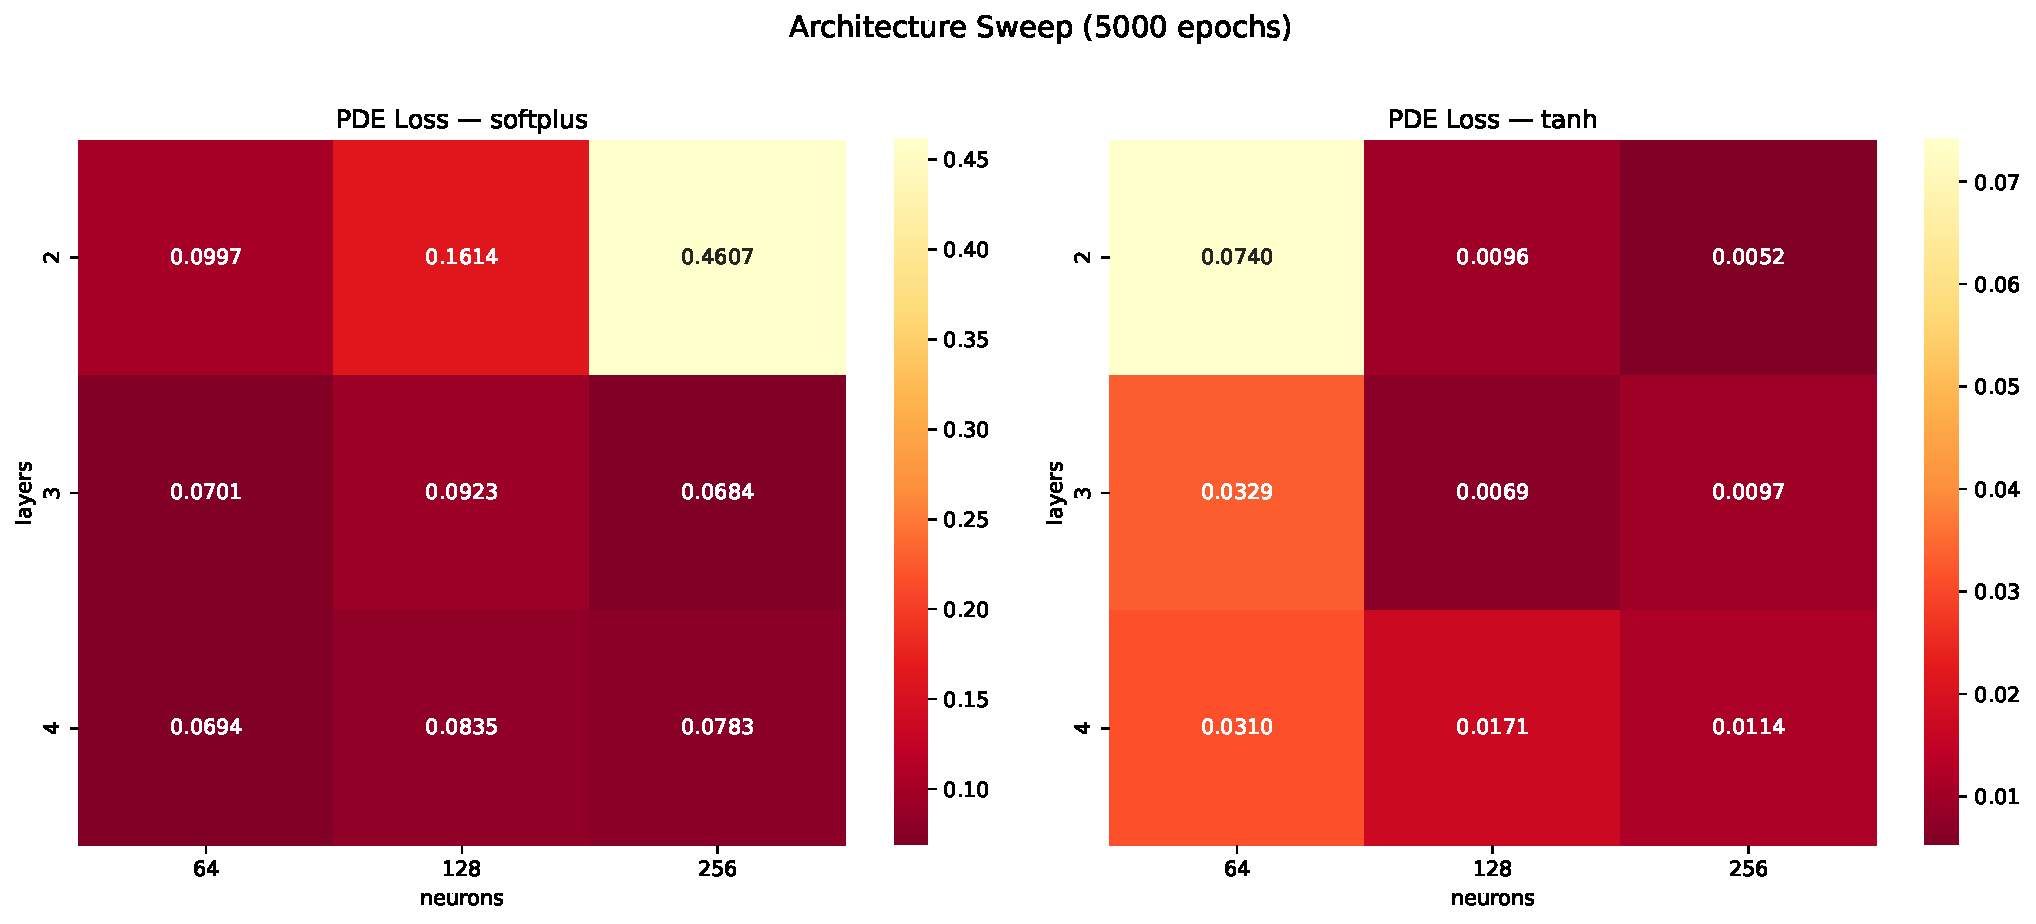
\includegraphics[width=\linewidth]{figures/hyper_bs_arch_heatmap.pdf}
    \caption{Architecture sweep for the Black--Scholes PINN after $5000$ epochs. The heatmaps compare PDE residual losses across different depths, widths, and activation functions. The $\tanh$ networks consistently outperform the corresponding \texttt{softplus} networks, indicating that the smoother bounded activation gives a better representation of the Black--Scholes price surface under this training setup.}
    \label{fig:hyper_bs_arch_heatmap.pdf}
\end{figure}

The architecture sweep shows a clear separation between activation functions. The best \texttt{softplus} models remain at PDE losses of order $10^{-2}$ to $10^{-1}$, while several $\tanh$ models reach losses around $10^{-3}$ to $10^{-2}$. The best architecture by PDE residual is the two-layer, $256$-neuron $\tanh$ network, with final PDE loss $5.193\times 10^{-3}$ after $5000$ epochs. The next-best candidates are the three-layer, $128$-neuron $\tanh$ model and the two-layer, $128$-neuron $\tanh$ model.

\begin{figure}[H]
    \centering
    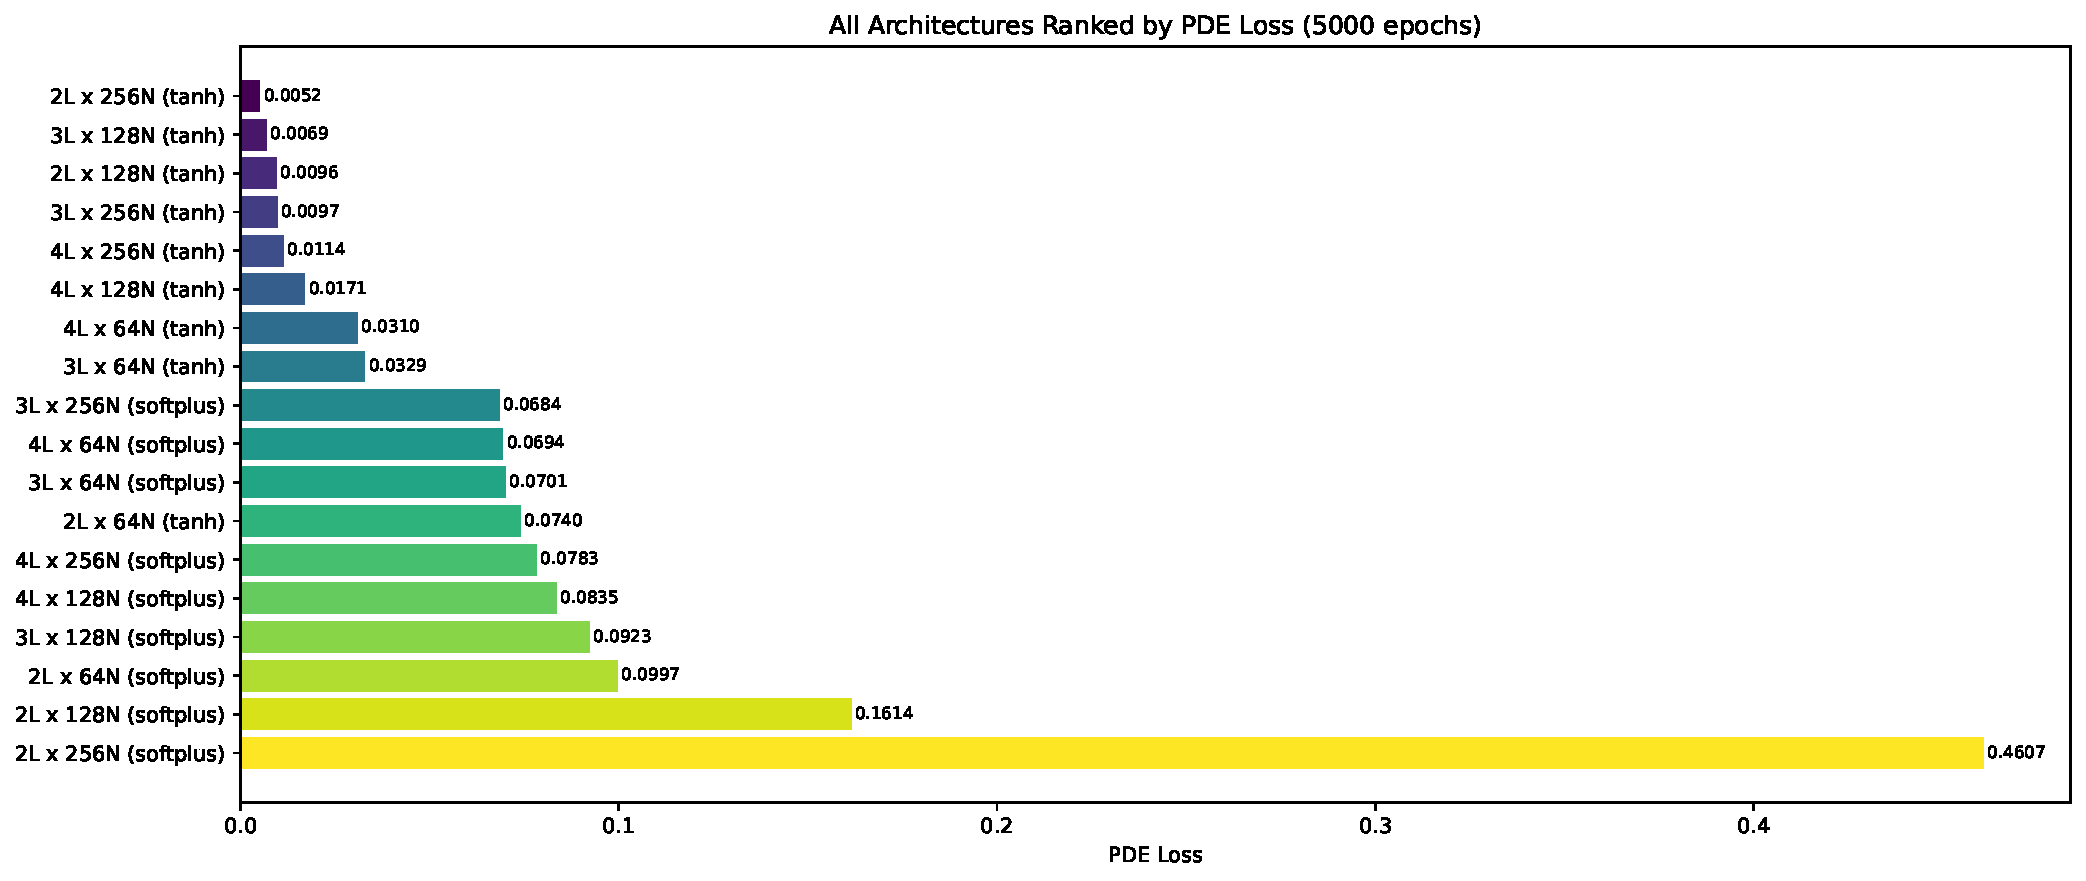
\includegraphics[width=\linewidth]{figures/hyper_bs_arch_ranked.pdf}
    \caption{Ranked architecture comparison for the Black--Scholes PINN. The best-performing model is the $2$-layer, $256$-neuron $\tanh$ network, followed by $3$ layers with $128$ neurons and $2$ layers with $128$ neurons. The ranking shows that increasing depth alone does not automatically improve the PINN; for this relatively low-dimensional PDE, a moderately shallow but sufficiently wide network performs best.}
    \label{fig:hyper_bs_arch_ranked.pdf}
\end{figure}

This result is consistent with the structure of the Black--Scholes problem. The solution surface is smooth for $\tau>0$, but contains sharp curvature near the strike and near expiry. A wider shallow network appears sufficient to capture this geometry without introducing the additional optimization difficulty associated with deeper architectures.

\subsubsection{Hyperparameters: learning rates}

Using the best architecture from the architecture sweep, the second sweep varied the learning rate over
\[
    10^{-4},\quad 3\times 10^{-4},\quad 5\times 10^{-4},
    \quad 10^{-3},\quad 3\times 10^{-3}.
\]
Each learning-rate candidate was trained for $5000$ epochs.

\begin{figure}[H]
    \centering
    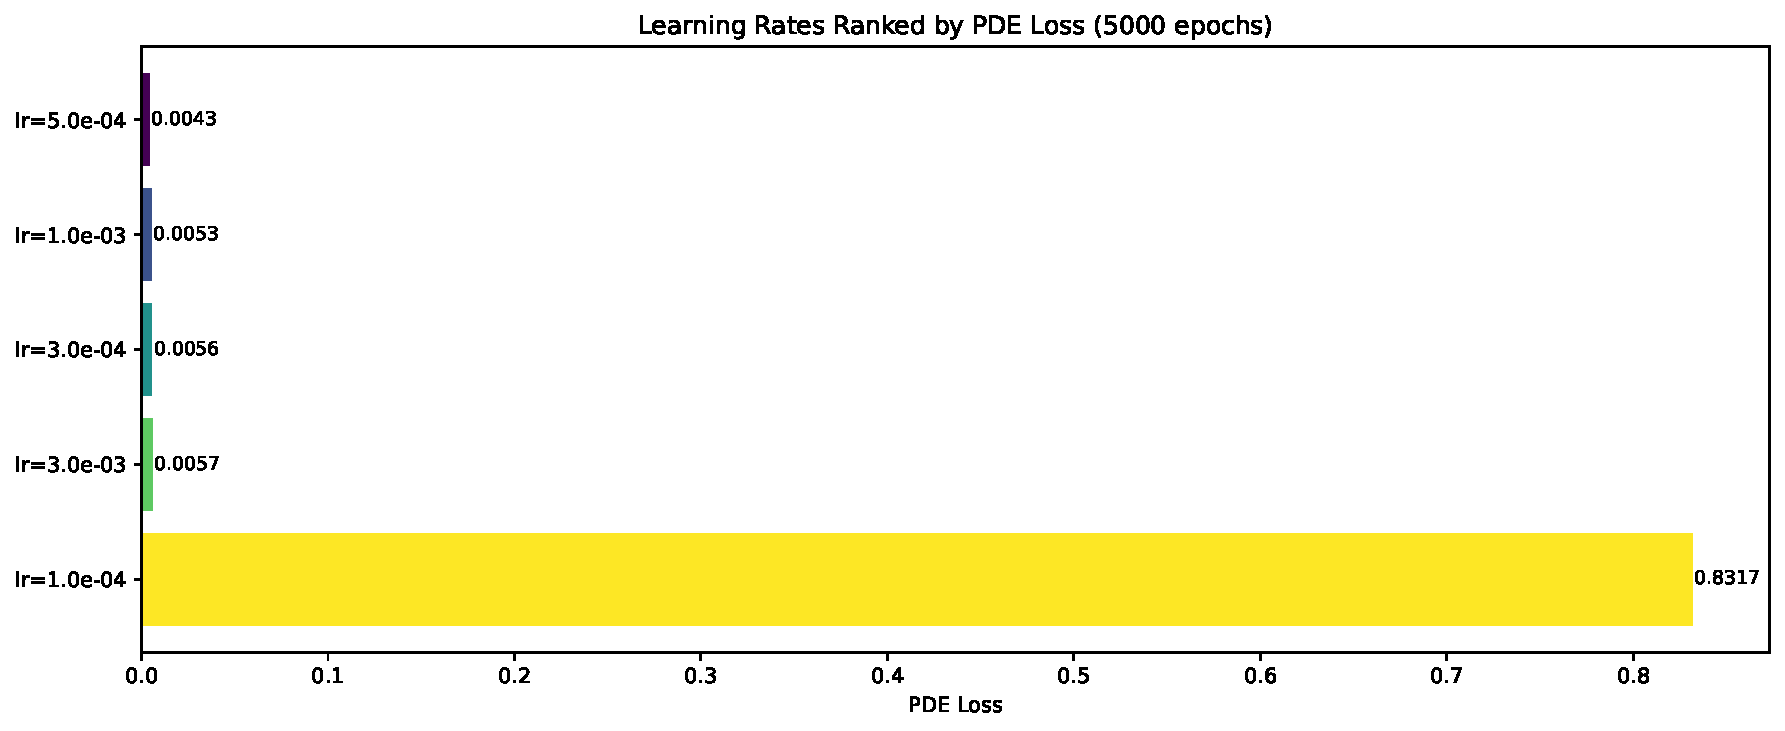
\includegraphics[width=\linewidth]{figures/hyper_bs_lr_ranked.pdf}
    \caption{Learning-rate sweep for the Black--Scholes PINN. The best PDE residual is obtained with learning rate $5\times 10^{-4}$, while $10^{-3}$, $3\times 10^{-4}$, and $3\times 10^{-3}$ also converge to similar values. The learning rate $10^{-4}$ performs substantially worse, indicating that it is too conservative over the fixed $5000$-epoch budget.}
    \label{fig:hyper_bs_lr_ranked.pdf}
\end{figure}

The best learning rate by PDE residual is $5\times 10^{-4}$, with final PDE loss $4.255\times 10^{-3}$. The neighboring values $10^{-3}$, $3\times 10^{-4}$, and $3\times 10^{-3}$ also perform well, all producing PDE losses of approximately $5\times 10^{-3}$. In contrast, $10^{-4}$ fails to converge sufficiently within the same epoch budget, producing a much larger PDE loss and a very large initial-condition error. This suggests that the optimization is not especially fragile within a moderate learning-rate range, but that too small a step size prevents the network from learning the payoff geometry quickly enough.

\subsubsection{Hyperparameters: loss weights}

The third sweep investigated the relative weighting of the PDE residual and initial-condition losses. The boundary weight was fixed at $\lambda_{\mathrm{bc}}=5$, while
\[
    \lambda_{\mathrm{pde}} \in \{10,15,20,25,30\},
    \qquad
    \lambda_{\mathrm{ic}} \in \{5,10,15,20\}.
\]
Each configuration was trained for $5000$ epochs.

\begin{figure}[H]
    \centering
    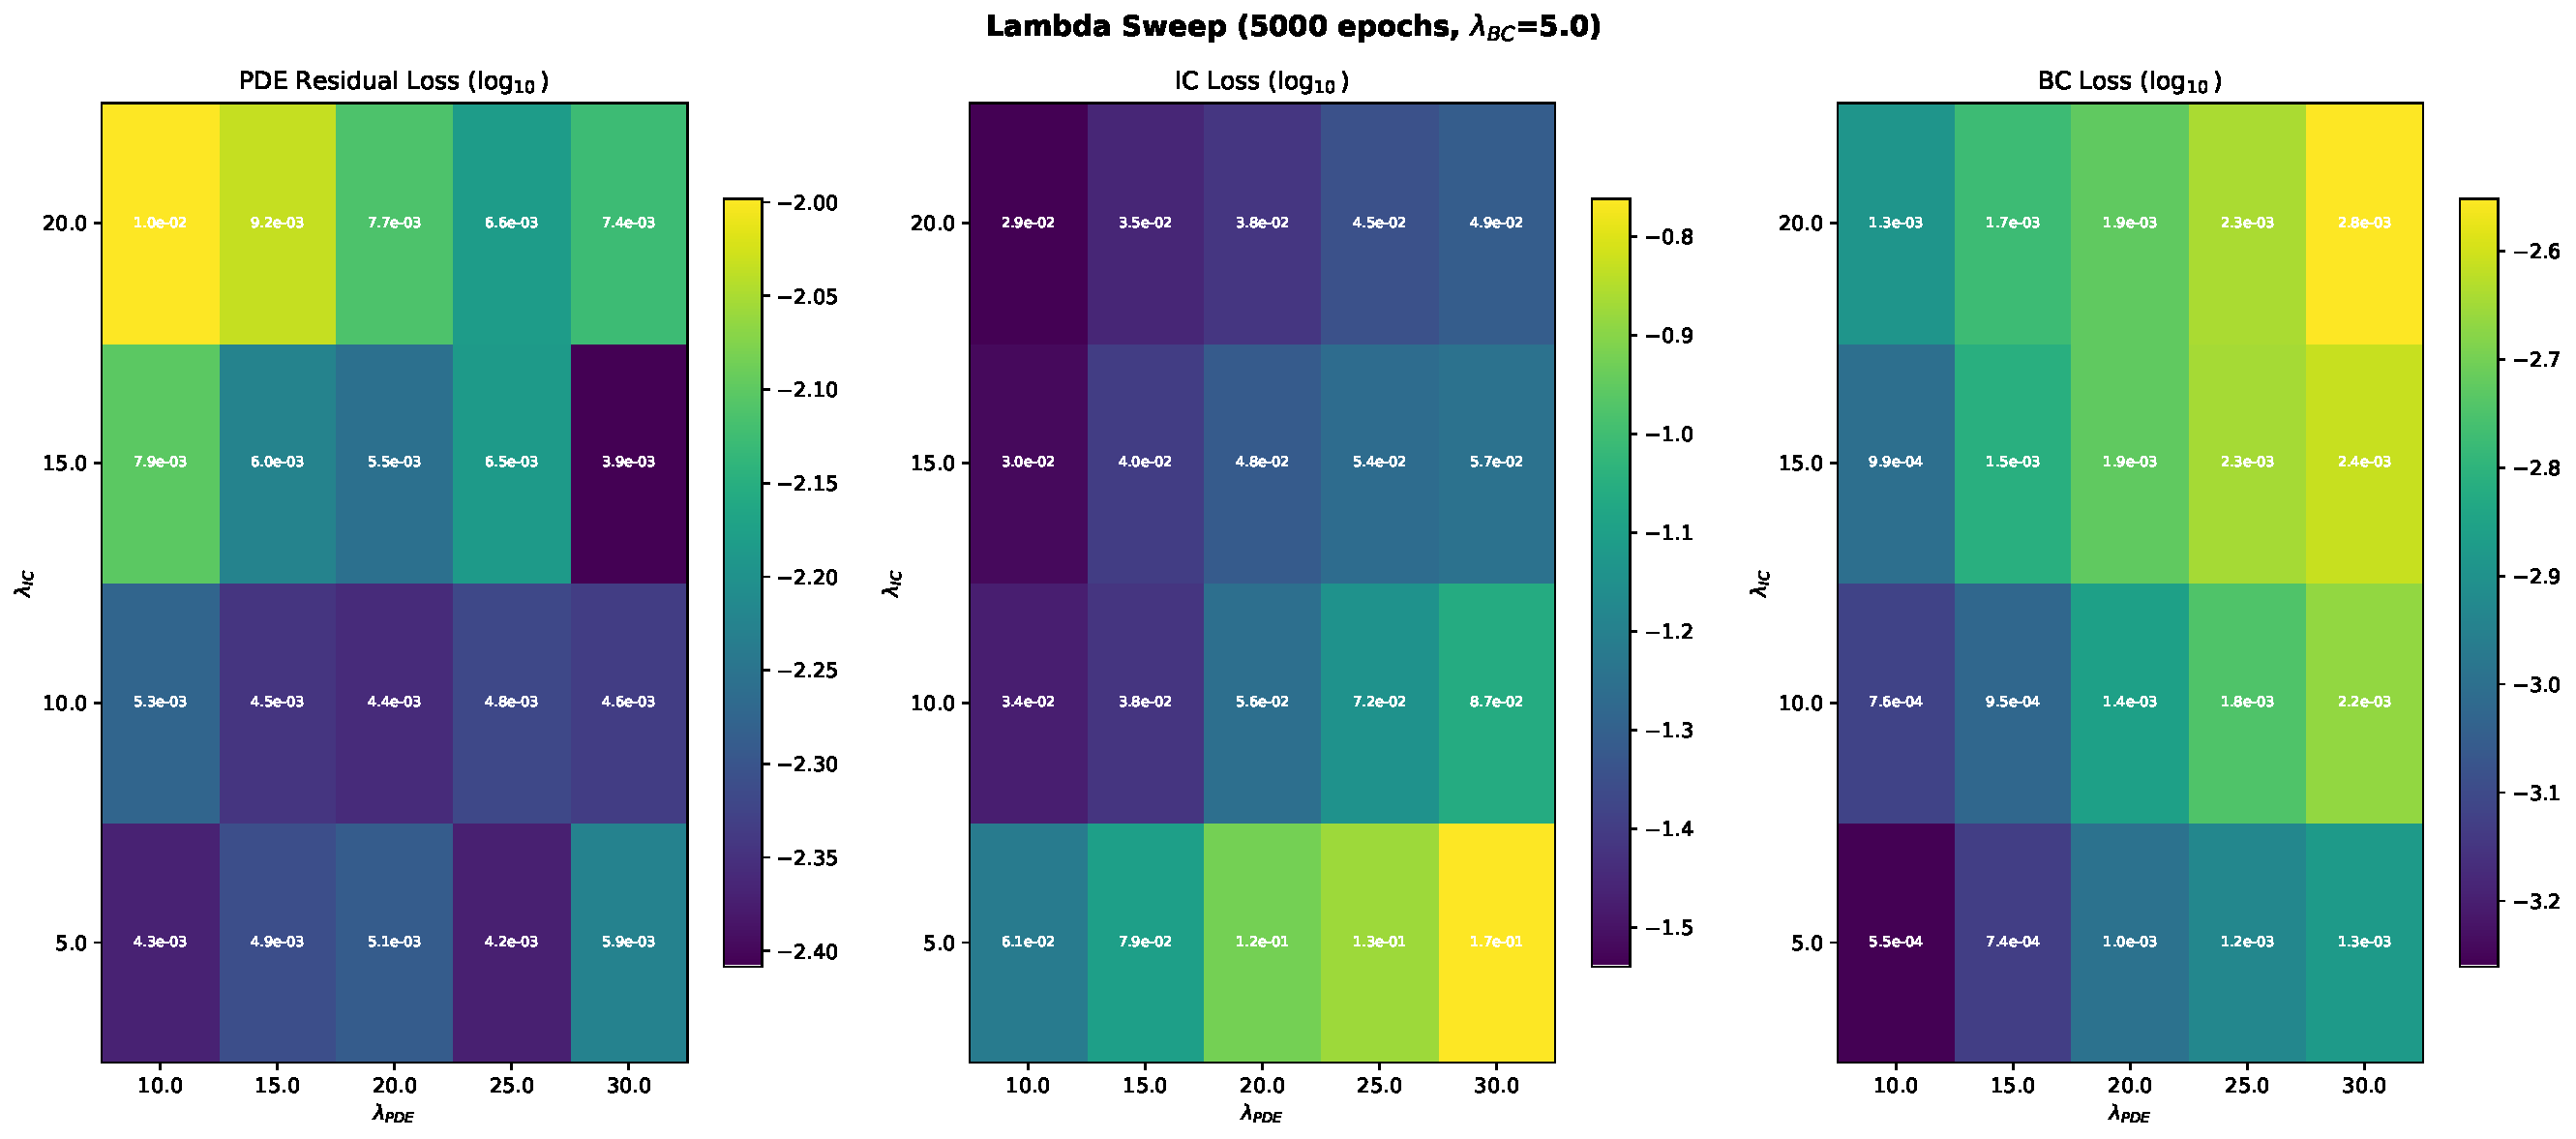
\includegraphics[width=\linewidth]{figures/hyper_bs_heatmap.pdf}
    \caption{Loss-weight sweep for the Black--Scholes PINN. The three heatmaps show the PDE residual, initial-condition loss, and boundary-condition loss over the tested values of $\lambda_{\mathrm{pde}}$ and $\lambda_{\mathrm{ic}}$, with $\lambda_{\mathrm{bc}}=5$ fixed. The results illustrate the trade-off between enforcing the differential equation and matching the terminal payoff condition.}
    \label{fig:hyper_bs_heatmap.pdf}
\end{figure}

The best PDE residual in the sweep is obtained at
\[
    \lambda_{\mathrm{pde}}=30,
    \qquad
    \lambda_{\mathrm{ic}}=15,
\]
with PDE loss $3.904\times 10^{-3}$. However, the sweep also shows that several nearby combinations perform similarly. For example, $(25,5)$ and $(10,5)$ both achieve PDE losses close to $4.25\times 10^{-3}$, while producing different balances between PDE satisfaction and payoff enforcement.

\begin{figure}[H]
    \centering
    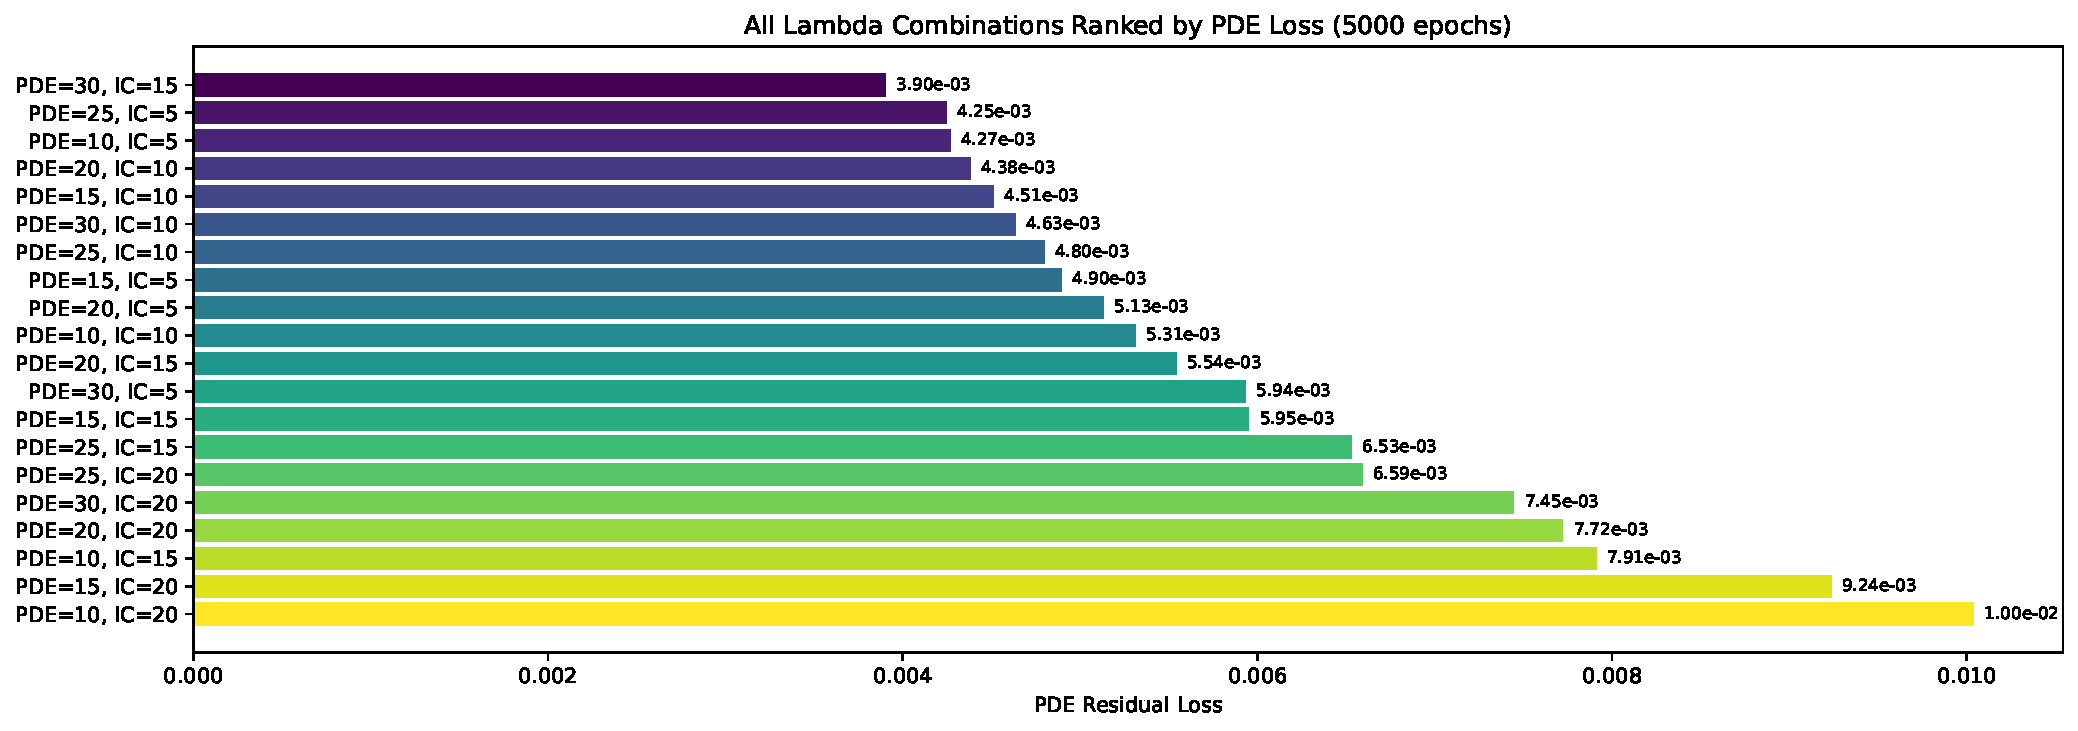
\includegraphics[width=\linewidth]{figures/hyper_bs_ranked.pdf}
    \caption{Ranked comparison of Black--Scholes loss-weight configurations. The lowest PDE residual is obtained for $(\lambda_{\mathrm{pde}},\lambda_{\mathrm{ic}})=(30,15)$, but several configurations lie in the same performance band. This indicates that the final result is not driven by a single unstable loss-weight choice, but by a reasonably broad region of workable training configurations.}
    \label{fig:hyper_bs_ranked.pdf}
\end{figure}

For the final model, the more moderate configuration
\[
    \lambda_{\mathrm{pde}}=10,
    \qquad
    \lambda_{\mathrm{ic}}=5,
    \qquad
    \lambda_{\mathrm{bc}}=5
\]
was retained. Although this was not the absolute best configuration by short-run PDE residual, it provided a stable and balanced training setup for the longer final run. This choice also avoids over-interpreting small differences from $5000$-epoch screening experiments, where optimizer noise and finite training duration can affect the ranking.

\subsubsection{Hyperparameters: convergence}

The fourth sweep examined the effect of training duration. The selected architecture, learning rate, and loss weights were fixed, while the epoch budget was varied over
\[
    1000,\quad 2000,\quad 3000,\quad 5000,\quad 7500,\quad 10000.
\]

\begin{figure}[H]
    \centering
    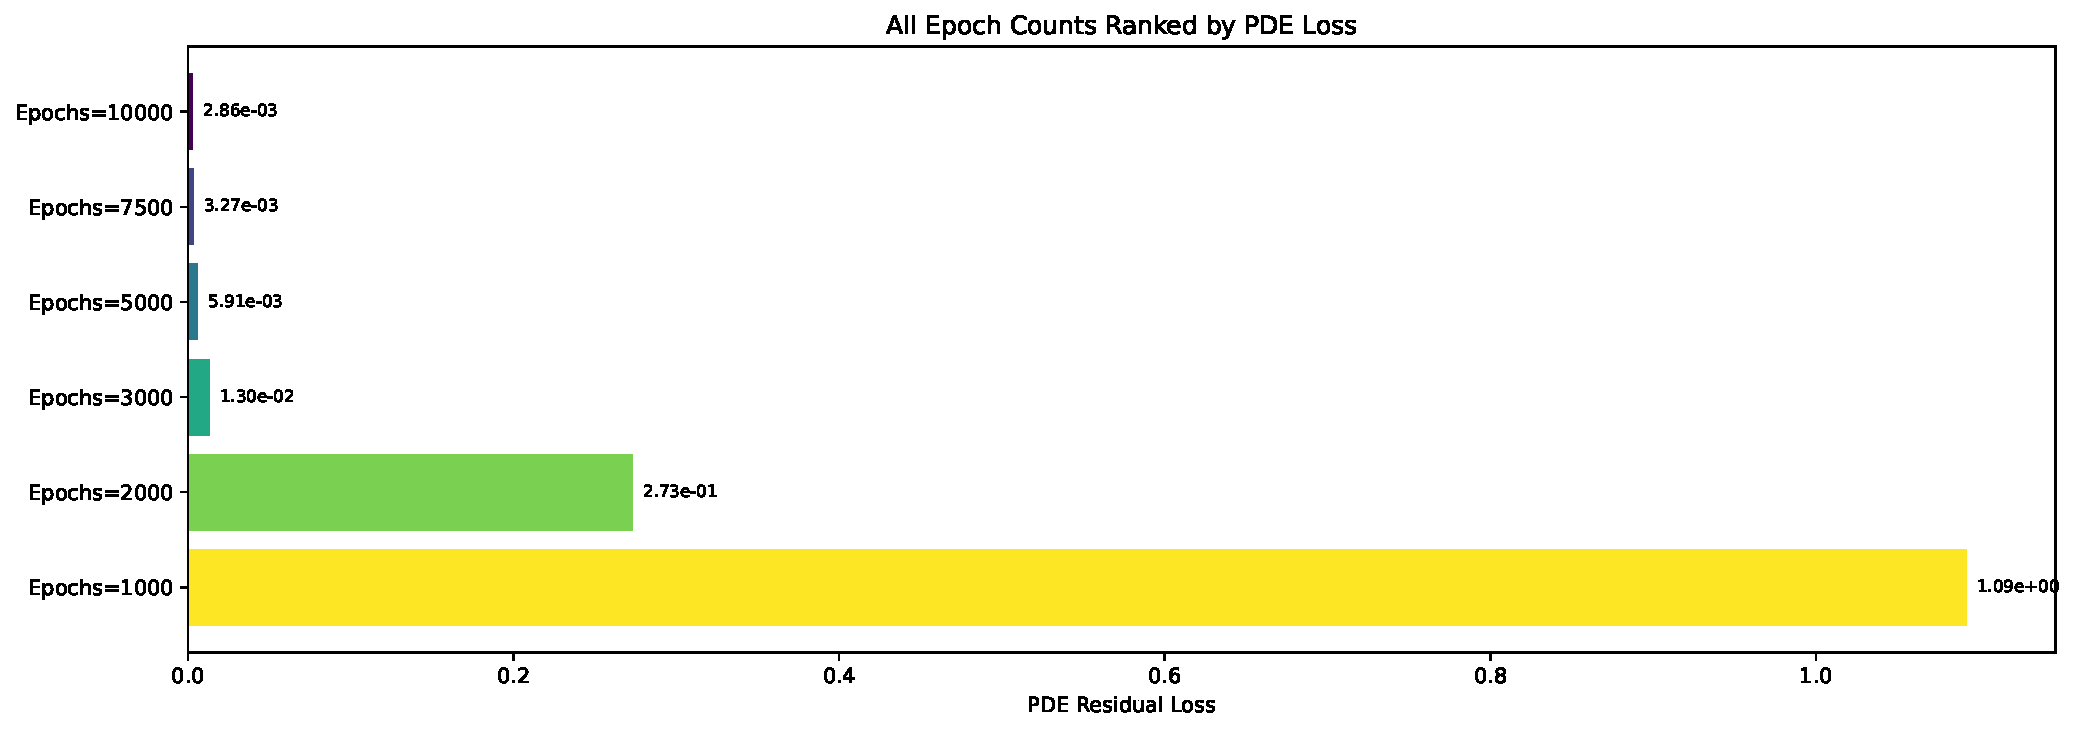
\includegraphics[width=\linewidth]{figures/hyper_bs_conv_ranked.pdf}
    \caption{Epoch-budget sweep for the Black--Scholes PINN. Longer training consistently improves the PDE residual over the tested range. The largest improvement occurs between $2000$ and $3000$ epochs, where the network transitions from a poor approximation of the payoff geometry to a substantially better PDE-consistent solution.}
    \label{fig:hyper_bs_conv_ranked.pdf}
\end{figure}

The convergence sweep shows that training duration is a first-order determinant of performance. At $1000$ epochs, the PDE loss remains above $1$, and the initial-condition loss is extremely large. By $3000$ epochs, the PDE loss falls to approximately $1.3\times 10^{-2}$, indicating that the network has begun to learn the relevant price geometry. Further training reduces the residual to $5.9\times 10^{-3}$ at $5000$ epochs, $3.3\times 10^{-3}$ at $7500$ epochs, and $2.9\times 10^{-3}$ at $10000$ epochs.

This motivated the final $50\,000$-epoch training run. The longer run was intended not only to reduce the PDE residual, but also to improve the terminal payoff fit and stabilize the higher-order derivatives used for Greek calculations.

\subsubsection{Final Black--Scholes PINN}

The final Black--Scholes PINN was trained for $50\,000$ epochs. Training took approximately $12$ minutes and $8$ seconds on a GPU runtime. The final total loss was $0.102625$, and the logged loss history shows a steady reduction in all major components. The PDE residual decreased from $4.019\times 10^{-2}$ at initialization to approximately $2.1\times 10^{-3}$ by the end of the printed training history, while the initial-condition loss fell from $4398.76$ to below $2\times 10^{-2}$. The boundary-condition loss remained small throughout the later stages of training.

\begin{figure*}[t]
    \centering
    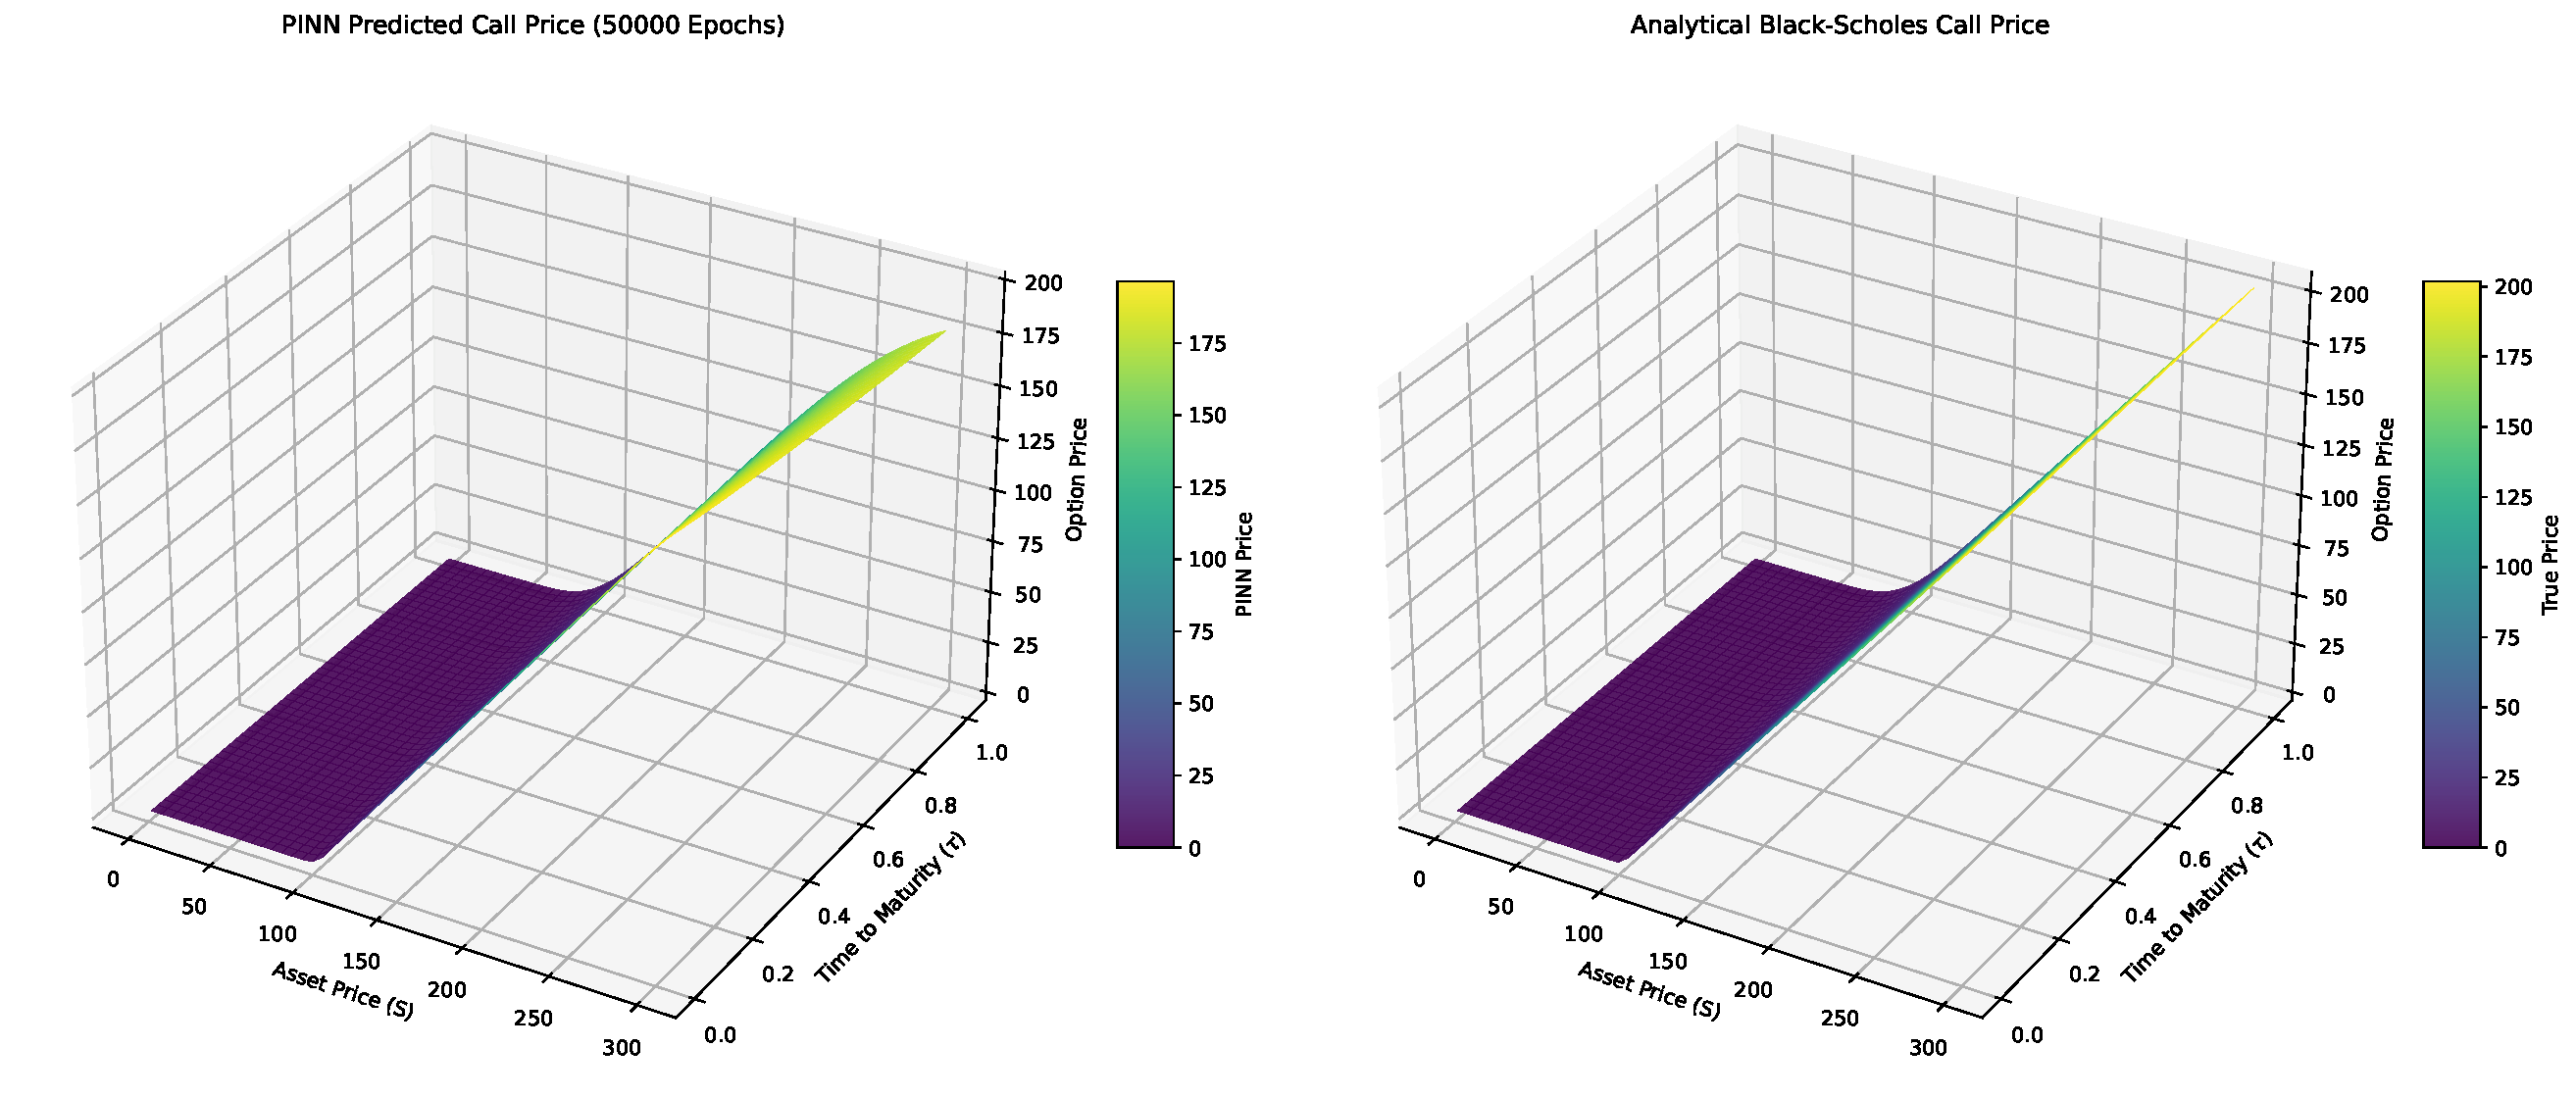
\includegraphics[width=0.95\textwidth]{figures/pinn_bs.pdf}
    \caption{Final Black--Scholes PINN solution after $50\,000$ training epochs, compared with the analytical Black--Scholes call-price surface. The learned surface captures the main continuation-value structure and closely reproduces the shape of the analytical benchmark. The largest qualitative challenge remains the high-curvature region near the strike and near expiry, where the terminal payoff kink must be approximated by a smooth neural network.}
    \label{fig:pinn_bs.pdf}
\end{figure*}

The final surface comparison shows that the PINN captures the global shape of the Black--Scholes call-price surface. The model reproduces the low-price out-of-the-money region, the approximately linear in-the-money region for large $S$, and the smooth transition around the strike. This is the main qualitative evidence that the network has internalized the diffusion structure of the Black--Scholes PDE rather than merely fitting isolated points.

Quantitatively, the model was evaluated at the at-the-money point $S=K=100$ with $\tau=0.5$. At this point, the PINN price is $6.927159$, compared with the analytical Black--Scholes value $6.888729$. This gives an absolute pricing error of
\[
    |V_{\mathrm{PINN}}-V_{\mathrm{BS}}|
    =
    |6.927159-6.888729|
    =
    0.038430.
\]
Relative to the analytical price, this corresponds to an error of approximately $0.56\%$. The PDE residual at the same point is $2.746582\times 10^{-3}$, indicating that the learned solution is locally close to satisfying the Black--Scholes equation.

\begin{table}[H]
    \centering
    \small
    \setlength{\tabcolsep}{6pt}
    \renewcommand{\arraystretch}{1.18}
    \caption{Black--Scholes PINN-estimated option price, selected Greeks, and PDE residual at $S=K=100$ and $\tau=0.5$. The analytical Black--Scholes price is included as a benchmark.}
    \label{tab:pinn_greeks}
    \begin{tabularx}{\linewidth}{@{} l X r @{}}
        \toprule
        \textbf{Quantity} & \textbf{Expression} & \textbf{PINN value} \\
        \midrule

        \multicolumn{3}{@{}l}{\textbf{Price level}} \\
        Price $(V)$
            & $V(S,\tau)$
            & $6.927159$ \\

        \addlinespace[0.25em]
        \multicolumn{3}{@{}l}{\textbf{First-order sensitivities}} \\
        Delta $(\Delta)$
            & $\partial V / \partial S$
            & $0.597287$ \\
        Theta $(\Theta)$
            & $\partial V / \partial \tau$
            & $8.053441$ \\
        Rho $(\rho)$
            & $\partial V / \partial r$
            & -- \\
        Phi $(\Phi)$
            & $\partial V / \partial q$
            & -- \\
        Vega
            & $\partial V / \partial \sigma$
            & -- \\

        \addlinespace[0.25em]
        \multicolumn{3}{@{}l}{\textbf{Second-order sensitivities}} \\
        Gamma $(\Gamma)$
            & $\partial^2 V / \partial S^2$
            & $0.027053$ \\
        Vomma
            & $\partial^2 V / \partial \sigma^2$
            & -- \\
        Vanna
            & $\partial^2 V / \partial S \partial \sigma$
            & -- \\
        Charm
            & $\partial^2 V / \partial S \partial \tau$
            & $0.093996$ \\

        \addlinespace[0.25em]
        \multicolumn{3}{@{}l}{\textbf{Third-order sensitivities}} \\
        Speed
            & $\partial^3 V / \partial S^3$
            & $-0.000629$ \\
        Zomma
            & $\partial^3 V / \partial S^2 \partial \sigma$
            & -- \\
        Color
            & $\partial^3 V / \partial S^2 \partial \tau$
            & $-0.027441$ \\

        \midrule
        \textbf{PDE residual}
            & Goal: $0.0$
            & $\mathbf{2.746582 \times 10^{-3}}$ \\
        \textbf{Analytical price}
            & Black--Scholes benchmark
            & $\mathbf{6.888729}$ \\
        \textbf{Absolute price error}
            & $|V_{\mathrm{PINN}}-V_{\mathrm{BS}}|$
            & $\mathbf{0.038430}$ \\
        \bottomrule
    \end{tabularx}
\end{table}

The Greek estimates are also internally consistent with the shape of the learned price surface. Delta is positive and below one, as expected for an at-the-money European call. Gamma is positive, reflecting the convexity of the option value with respect to the underlying asset price. The third-order derivatives are small in magnitude but nonzero, showing that automatic differentiation can extract higher-order structure from the trained network.

The unavailable entries in \cref{tab:pinn_greeks} are not failures of the PINN itself. They reflect the fact that the trained Black--Scholes network takes $(S,\tau)$ as inputs, while $r$, $q$, and $\sigma$ are fixed external parameters rather than differentiable input coordinates. Therefore, parameter Greeks such as Rho and Vega are not directly available from this particular trained network. They could be obtained either by training a parameterized PINN with $(S,\tau,r,\sigma)$ as inputs, or by using external bump-and-revalue calculations.

Overall, the Black--Scholes experiment is successful. The PINN learns a visually accurate price surface, achieves a small local PDE residual, produces a sub-percent pointwise pricing error at the benchmark evaluation point, and yields meaningful state-variable Greeks through automatic differentiation. At the same time, the experiment reveals the practical sensitivity of PINNs to architecture, activation function, learning rate, loss weighting, and training duration. This motivates the more careful interpretation required in the Heston and inverse-calibration experiments, where the PDE and optimization landscape are substantially more difficult.

\clearpage
\subsection{Heston}

The Heston experiment extends the PINN framework from the two-dimensional Black--Scholes domain $(S,\tau)$ to the three-dimensional stochastic-volatility domain $(S,v,\tau)$. This is a substantially harder problem. The network must now learn how the option price changes not only with asset price and time to maturity, but also with the instantaneous variance state variable. In addition, the Heston PDE contains a mixed derivative term $\partial^2 V/\partial S \partial v$, which makes the differential constraint more demanding than in the Black--Scholes case.

The Heston parameters were fixed at
\[
    \kappa = 2.0,
    \qquad
    \theta = 0.04,
    \qquad
    \xi = 0.3,
    \qquad
    \rho = -0.7,
\]
with $K=100$, $r=0.05$, $v_0=0.04$, $S_{\max}=300$, and $\tau_{\max}=1.0$. The collocation data consisted of $10\,000$ interior points, $2000$ initial-condition points, and boundary points sampled along the edges of the computational domain. As in the Black--Scholes experiment, the Heston model was first tuned through architecture, learning-rate, loss-weight, and convergence sweeps before training a final long-run PINN.

The final Heston PINN was trained for $50\,000$ epochs using a three-hidden-layer network with $256$ neurons per layer, $\tanh$ activation, learning rate $5\times 10^{-3}$, and loss weights
\[
    \lambda_{\mathrm{pde}}=10,
    \qquad
    \lambda_{\mathrm{ic}}=10,
    \qquad
    \lambda_{\mathrm{bc}}=5.
\]
For the final training run, the boundary-condition loss was imposed on the lower asset-price boundary $S=0$, where the call option value is known to vanish.

\subsubsection{Hyperparameters: architecture}

The architecture sweep tested the same grid of depths, widths, and activation functions used in the Black--Scholes experiment: $2$, $3$, or $4$ hidden layers; $64$, $128$, or $256$ neurons per layer; and either \texttt{softplus} or $\tanh$ activation. Each model was trained for $5000$ epochs using the same baseline Heston parameters and loss weights.

\begin{figure}[H]
    \centering
    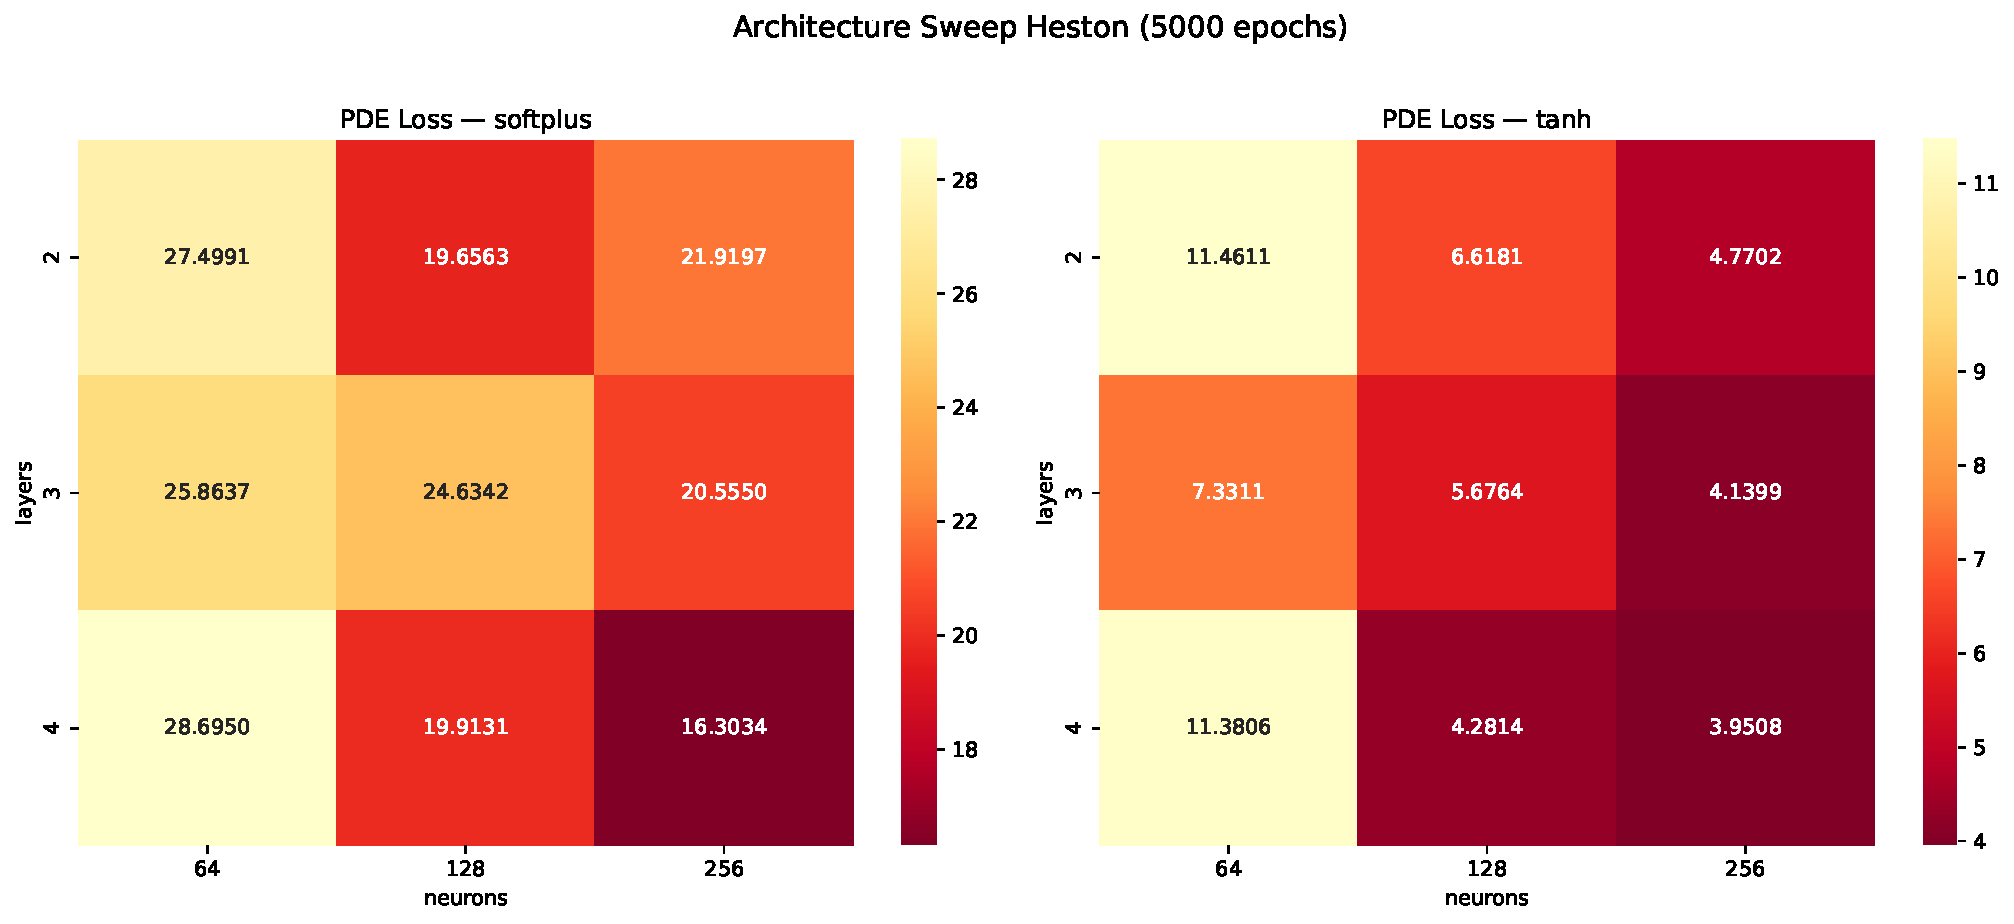
\includegraphics[width=\linewidth]{figures/hyper_hs_arch_heatmap.pdf}
    \caption{Architecture sweep for the Heston PINN after $5000$ epochs. The heatmaps compare PDE residual losses across depths, widths, and activation functions. As in the Black--Scholes case, $\tanh$ activations substantially outperform \texttt{softplus}. The best-performing models are wider $\tanh$ networks, reflecting the increased representational demands of the three-dimensional Heston price surface.}
    \label{fig:hyper_hs_arch_heatmap.pdf}
\end{figure}

The architecture results show a much sharper difficulty increase relative to Black--Scholes. Whereas the best Black--Scholes architecture achieved PDE losses of order $10^{-3}$ after $5000$ epochs, the best Heston architecture remains at order $1$. This is expected: the Heston PDE is higher-dimensional, contains variance dynamics, and includes the mixed derivative term generated by correlation between the asset and variance Brownian motions.

The best architecture by PDE residual is the four-layer, $256$-neuron $\tanh$ model, with PDE loss $3.950807$. However, the three-layer, $256$-neuron $\tanh$ network is very close, reaching PDE loss $4.139890$, while being somewhat less computationally expensive. The final model therefore uses the three-layer, $256$-neuron $\tanh$ architecture as a practical compromise between accuracy and training cost.

A second important observation is that all \texttt{softplus} networks perform poorly relative to the $\tanh$ networks. The best \texttt{softplus} architecture gives PDE loss $16.303411$, far above the leading $\tanh$ models. This suggests that, under the present setup, $\tanh$ provides a more effective basis for representing the Heston price surface and its derivatives.

\subsubsection{Hyperparameters: learning rate}

The learning-rate sweep was performed using the selected $\tanh$ architecture with three hidden layers and $256$ neurons per layer. The tested learning rates were
\[
    10^{-2},
    \quad
    5\times 10^{-3},
    \quad
    10^{-3},
    \quad
    5\times 10^{-4},
    \quad
    10^{-4}.
\]
Each run was trained for $5000$ epochs.

\begin{figure}[H]
    \centering
    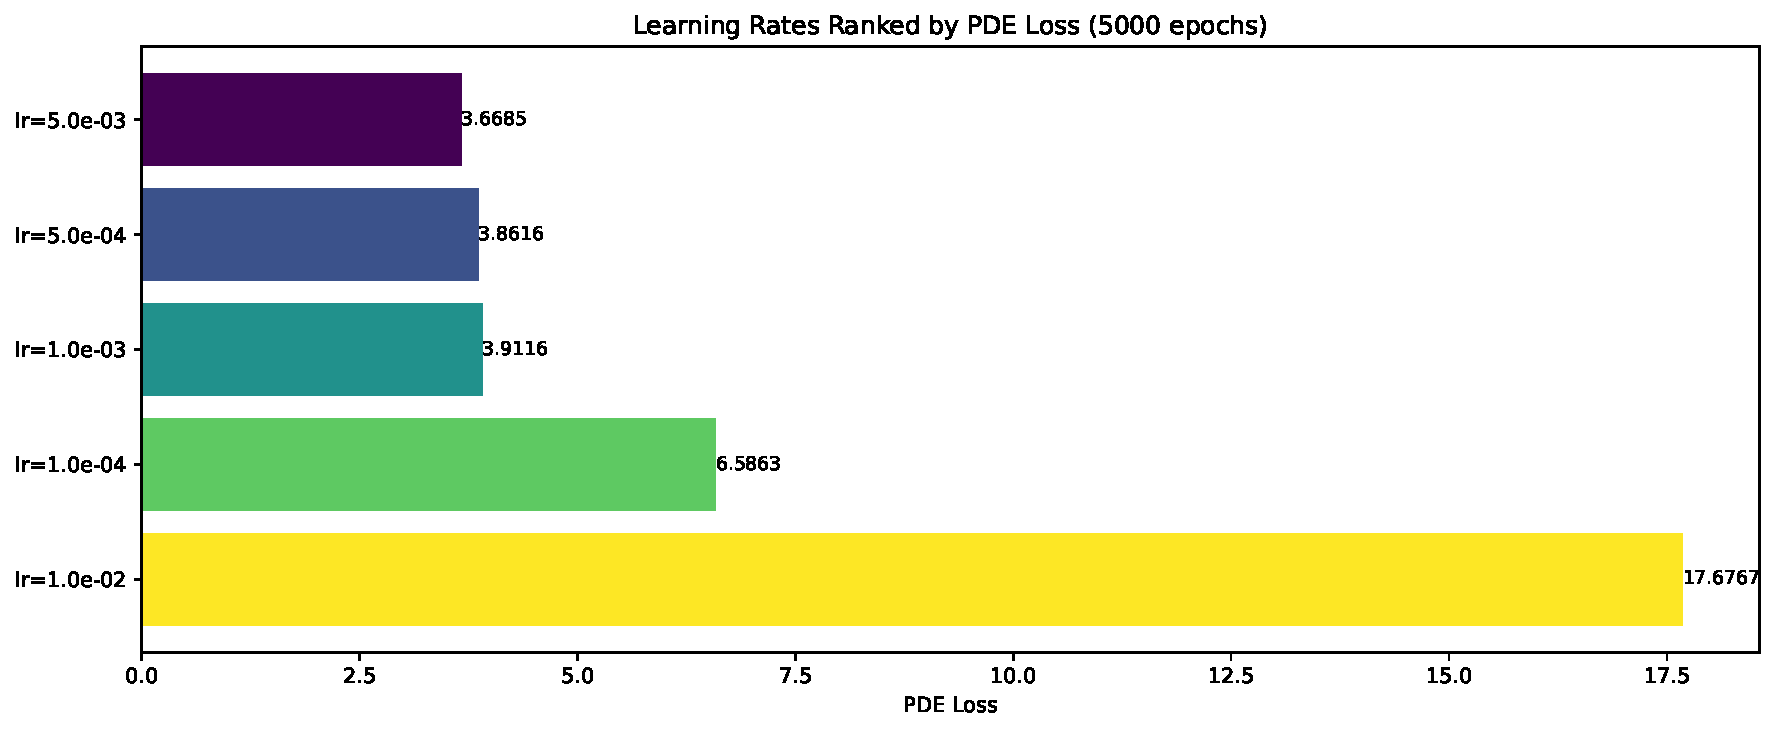
\includegraphics[width=\linewidth]{figures/hyper_hs_lr_ranked.pdf}
    \caption{Learning-rate sweep for the Heston PINN. The best PDE residual is obtained with learning rate $5\times 10^{-3}$. Lower learning rates converge more slowly over the fixed epoch budget, while $10^{-2}$ is too aggressive and leads to substantially worse PDE residual performance.}
    \label{fig:hyper_hs_lr_ranked.pdf}
\end{figure}

The best learning rate is $5\times 10^{-3}$, giving PDE loss $3.668460$ after $5000$ epochs. The learning rates $5\times 10^{-4}$ and $10^{-3}$ also perform reasonably, with PDE losses $3.861612$ and $3.911578$, respectively. In contrast, $10^{-4}$ is too slow for the fixed training budget, while $10^{-2}$ appears too aggressive and produces a much larger PDE loss of $17.676699$.

This result differs from the Black--Scholes case, where several moderate learning rates performed similarly. For Heston, the optimization landscape is more sensitive. The model needs a sufficiently large learning rate to escape the initially poor payoff approximation, but not so large that the PDE residual becomes unstable. The value $5\times 10^{-3}$ was therefore used in the subsequent Heston experiments.

\subsubsection{Hyperparameters: loss weights}

The loss-weight sweep varied the PDE and initial-condition weights while holding the boundary-condition weight fixed:
\[
    \lambda_{\mathrm{pde}} \in \{10,15,20,25,30\},
    \qquad
    \lambda_{\mathrm{ic}} \in \{5,10,15,20\},
    \qquad
    \lambda_{\mathrm{bc}}=5.
\]
Each configuration was trained for $5000$ epochs.

\begin{figure}[H]
    \centering
    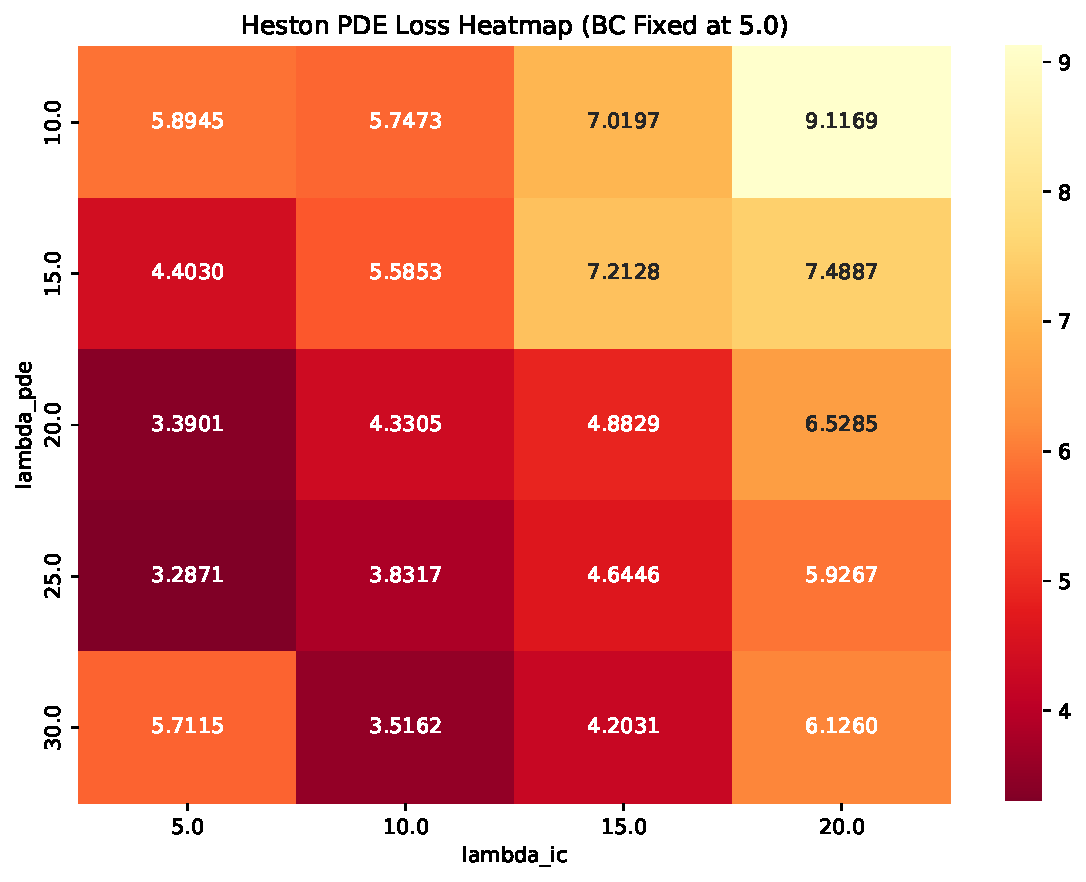
\includegraphics[width=\linewidth]{figures/hyper_hs_lambda_heatmap.pdf}
    \caption{Loss-weight sweep for the Heston PINN with $\lambda_{\mathrm{bc}}=5$ fixed. The heatmap reports the final PDE residual loss for each tested pair $(\lambda_{\mathrm{pde}},\lambda_{\mathrm{ic}})$. The best short-run PDE residual is obtained near $\lambda_{\mathrm{pde}}=25$ and $\lambda_{\mathrm{ic}}=5$, although the final model uses a more balanced weighting to stabilize the longer training run.}
    \label{fig:hyper_hs_lambda_heatmap.pdf}
\end{figure}

The lowest PDE residual in the sweep is achieved at
\[
    \lambda_{\mathrm{pde}}=25,
    \qquad
    \lambda_{\mathrm{ic}}=5,
\]
with PDE loss $3.287135$. The neighboring configuration $(20,5)$ is also competitive, with PDE loss $3.390135$. These results indicate that, in short training runs, emphasizing the PDE residual more strongly than the initial condition improves interior equation satisfaction.

However, the Heston problem requires a more careful balance than the Black--Scholes benchmark. A configuration that minimizes the PDE loss over $5000$ epochs does not necessarily produce the best final surface or the most stable long-run training. The final model therefore uses
\[
    \lambda_{\mathrm{pde}}=10,
    \qquad
    \lambda_{\mathrm{ic}}=10,
    \qquad
    \lambda_{\mathrm{bc}}=5,
\]
which gives a more balanced treatment of the PDE residual and terminal payoff during the full $50\,000$-epoch training run. This is especially important because the payoff condition remains difficult to enforce in the higher-dimensional Heston setting.

\subsubsection{Hyperparameters: convergence}

The convergence sweep fixed the architecture, learning rate, and loss weights, while varying the number of training epochs:
\[
    5000,
    \quad
    10000,
    \quad
    15000,
    \quad
    20000,
    \quad
    25000.
\]

\begin{figure}[H]
    \centering
    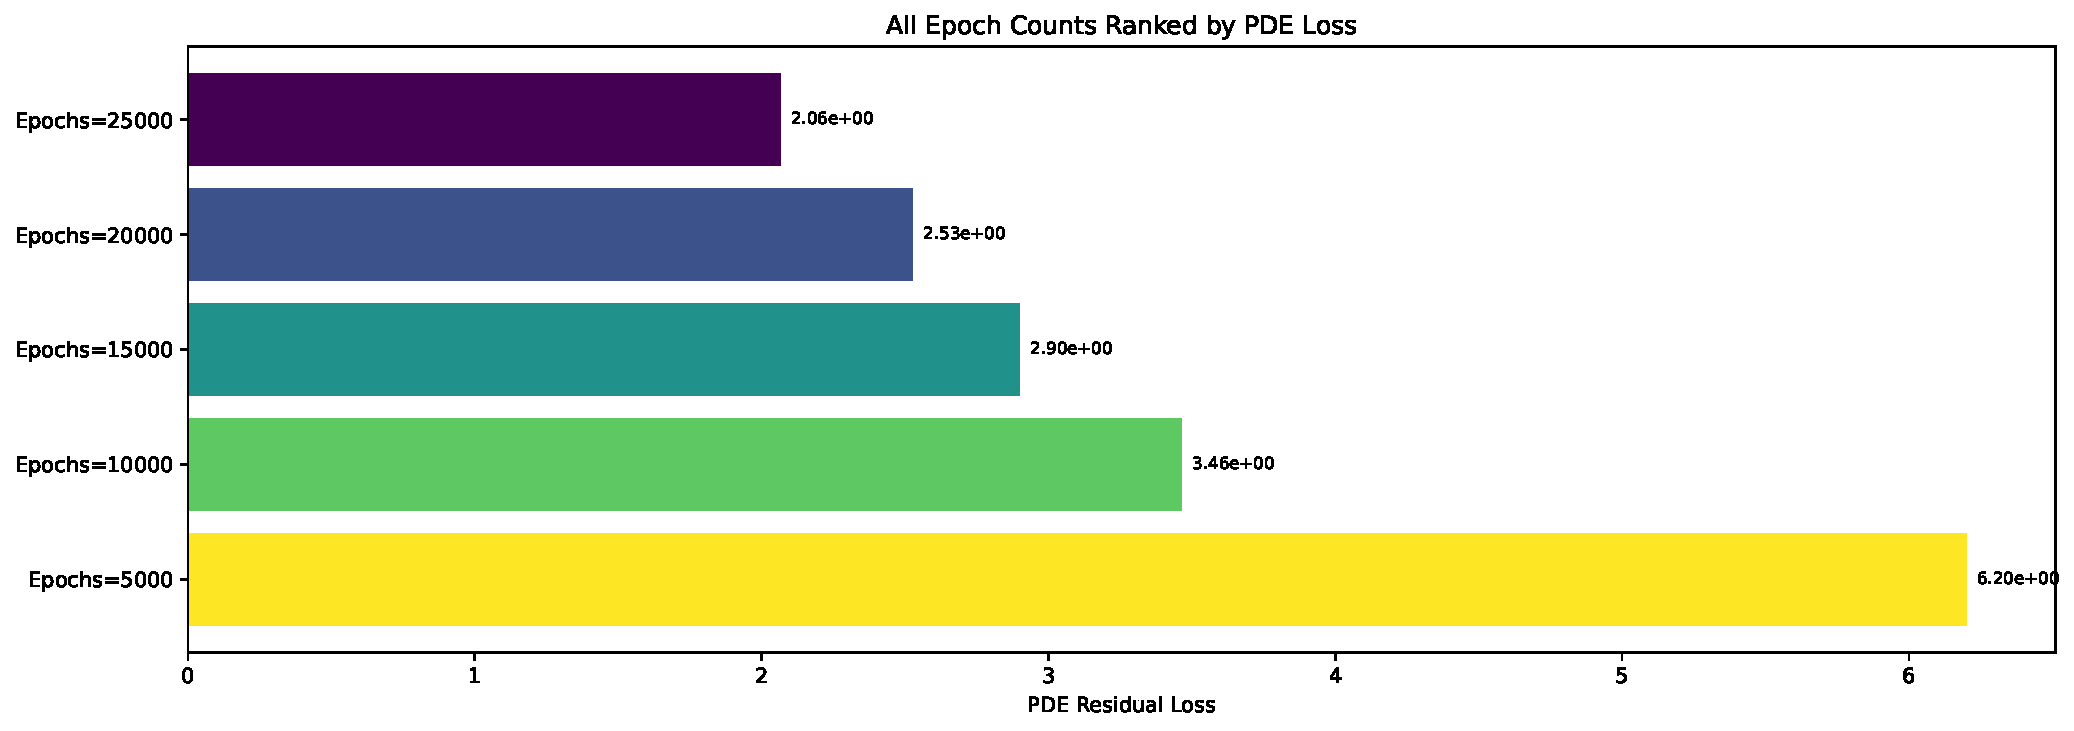
\includegraphics[width=\linewidth]{figures/hyper_hs_conv_ranked.pdf}
    \caption{Epoch-budget sweep for the Heston PINN. Longer training consistently improves the PDE residual over the tested range, although the residual remains much larger than in the Black--Scholes experiment. This reflects the additional dimensionality, variance dependence, and mixed derivative term in the Heston PDE.}
    \label{fig:hyper_hs_conv_ranked.pdf}
\end{figure}

The convergence results show a monotonic improvement in PDE residual as training duration increases. The PDE loss falls from $6.199924$ after $5000$ epochs to $3.463765$ after $10\,000$ epochs, and further to $2.064686$ after $25\,000$ epochs. The initial-condition loss and total loss also decrease over the same range.

This confirms that the Heston PINN benefits materially from longer optimization. The higher-dimensional PDE does not converge as rapidly as the Black--Scholes model, and the short-run sweeps therefore understate the quality that can be achieved with longer training. This motivated the final $50\,000$-epoch training run.

\clearpage
\subsubsection{Final Heston PINN}

The final Heston PINN was trained for $50\,000$ epochs. Training took approximately $23$ minutes and $30$ seconds on a GPU runtime. The final run used $10\,000$ interior collocation points, $2000$ initial-condition points, and $250$ lower-boundary points at $S=0$. The final total loss was $0.384823$.

The loss history shows that the Heston optimization is less smooth than the Black--Scholes case. The PDE and initial-condition losses exhibit occasional spikes during training, especially in the earlier and middle parts of the run. Nevertheless, the overall trend is strongly downward. By the later stages, the model reaches substantially lower PDE, initial-condition, and boundary losses than in the short hyperparameter sweeps. This supports the interpretation that the Heston PINN is trainable, but more sensitive to optimization dynamics than the Black--Scholes PINN.

\begin{figure}[H]
    \centering
    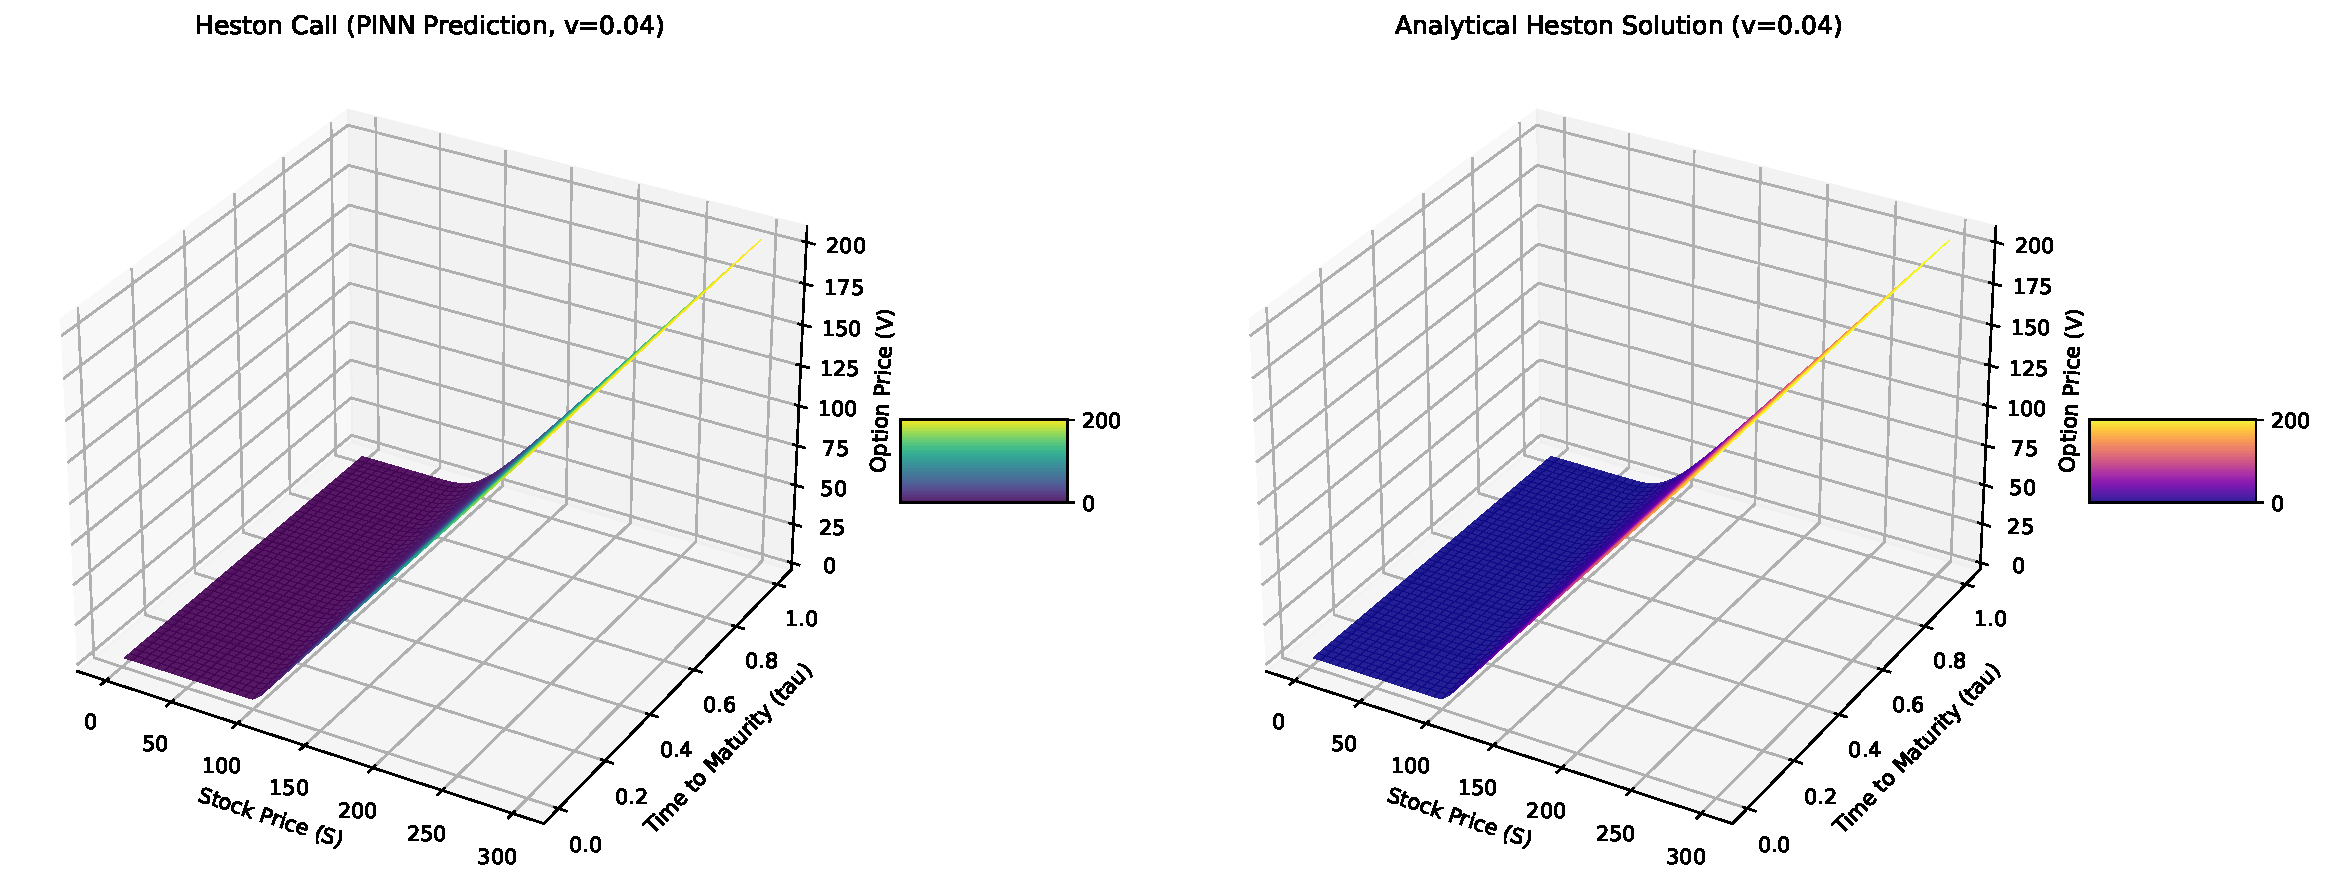
\includegraphics[width=\textwidth]{figures/pinn_hs.pdf}
    \caption{Final Heston PINN solution after $50\,000$ training epochs, evaluated on the slice $v=v_0=0.04$ and compared with the semi-analytical Heston reference solution. The PINN captures the global structure of the Heston call-price surface, including the low-value out-of-the-money region and the increasing in-the-money region. The comparison is shown on a fixed-variance slice, so the full three-dimensional dependence on $(S,v,\tau)$ is only partially visualized.}
    \label{fig:pinn_hs.pdf}
\end{figure}

The final surface comparison indicates that the Heston PINN captures the main structure of the semi-analytical Heston solution on the slice $v=v_0=0.04$. The learned surface has the correct qualitative shape: option values are close to zero in deep out-of-the-money regions, increase with the underlying asset price, and vary smoothly with time to maturity. As expected, the surface is harder to learn than in the Black--Scholes case, since the plotted slice represents only one cross-section of a higher-dimensional learned function.

The model was evaluated quantitatively at the at-the-money point
\[
    S=K=100,
    \qquad
    v=v_0=0.04,
    \qquad
    \tau=0.5.
\]
At this point, the PINN predicts
\[
    V_{\mathrm{PINN}} = 6.830489,
\]
while the semi-analytical Heston benchmark gives
\[
    V_{\mathrm{Heston}} = 6.837137.
\]
The absolute pricing error is therefore
\[
    |V_{\mathrm{PINN}}-V_{\mathrm{Heston}}|
    =
    0.006648,
\]
corresponding to a relative error of approximately $0.10\%$. This is a strong pointwise pricing result, especially given the increased dimensionality of the Heston problem.

\begin{table}[H]
    \centering
    \small
    \setlength{\tabcolsep}{6pt}
    \renewcommand{\arraystretch}{1.18}
    \caption{Heston PINN-estimated option price, selected Greeks, and PDE residual at $S=K=100$, $v=v_0=0.04$, and $\tau=0.5$. The semi-analytical Heston price is included as the benchmark.}
    \label{tab:heston_pinn_greeks}
    \begin{tabularx}{\linewidth}{@{} l X r @{}}
        \toprule
        \textbf{Quantity} & \textbf{Expression} & \textbf{PINN value} \\
        \midrule

        \multicolumn{3}{@{}l}{\textbf{Price level}} \\
        Price $(V)$
            & $V(S,v,\tau)$
            & $6.830489$ \\

        \addlinespace[0.25em]
        \multicolumn{3}{@{}l}{\textbf{First-order sensitivities}} \\
        Delta $(\Delta)$
            & $\partial V / \partial S$
            & $0.645494$ \\
        Vega$_v$
            & $\partial V / \partial v$
            & $42.177811$ \\
        Theta $(\Theta)$
            & $\partial V / \partial \tau$
            & $8.028887$ \\

        \addlinespace[0.25em]
        \multicolumn{3}{@{}l}{\textbf{Second-order sensitivities}} \\
        Gamma $(\Gamma)$
            & $\partial^2 V / \partial S^2$
            & $0.026912$ \\
        Volga$_v$
            & $\partial^2 V / \partial v^2$
            & $-286.995544$ \\
        Vanna$_v$
            & $\partial^2 V / \partial S \partial v$
            & $-0.408809$ \\
        Charm
            & $\partial^2 V / \partial S \partial \tau$
            & $0.131729$ \\

        \addlinespace[0.25em]
        \multicolumn{3}{@{}l}{\textbf{Third-order sensitivities}} \\
        Speed
            & $\partial^3 V / \partial S^3$
            & $-0.001735$ \\
        Zomma$_v$
            & $\partial^3 V / \partial S^2 \partial v$
            & $-0.210728$ \\
        Color
            & $\partial^3 V / \partial S^2 \partial \tau$
            & $-0.032710$ \\

        \midrule
        \textbf{PDE residual}
            & Goal: $0.0$
            & $\mathbf{-6.628036 \times 10^{-2}}$ \\
        \textbf{Analytical price}
            & Semi-analytical Heston benchmark
            & $\mathbf{6.837137}$ \\
        \textbf{PINN error}
            & $|V_{\mathrm{PINN}} - V_{\mathrm{Heston}}|$
            & $\mathbf{0.006648}$ \\
        \bottomrule
    \end{tabularx}
\end{table}

The Greek estimates are qualitatively reasonable. Delta is positive and below one, as expected for an at-the-money call. Gamma is positive, indicating local convexity with respect to the underlying asset price. The variance sensitivity Vega$_v$ is large and positive, consistent with the intuition that higher instantaneous variance increases the value of optionality. The negative Volga$_v$ indicates concavity of the learned price surface in the local variance direction at the evaluation point.

At the same time, the Heston results should be interpreted more cautiously than the Black--Scholes results. The pointwise pricing error is very small, but the local PDE residual is $-6.628036\times 10^{-2}$, which is larger in magnitude than the Black--Scholes residual. This gap highlights an important feature of PINNs: accurate pricing at a selected point does not necessarily imply equally strong global PDE satisfaction. In the Heston setting, the model can learn an accurate local price while still finding it difficult to fully satisfy the higher-dimensional PDE everywhere.

The Heston experiment is therefore successful, but less clean than the Black--Scholes benchmark. The final PINN achieves an excellent pointwise price match to the semi-analytical Heston solution and produces meaningful state-variable Greeks through automatic differentiation. However, the hyperparameter sweeps and loss history show that the optimization landscape is substantially more difficult. The model requires wider networks, larger learning rates, longer training, and careful interpretation of residual diagnostics. This provides the natural bridge to the inverse calibration problem, where the difficulty increases further because the Heston parameters themselves must be learned from data.


\clearpage\subsection{Inverse problem}

\subsubsection{Hyperparameters: lambda values}

\begin{figure}[H]
    \centering
    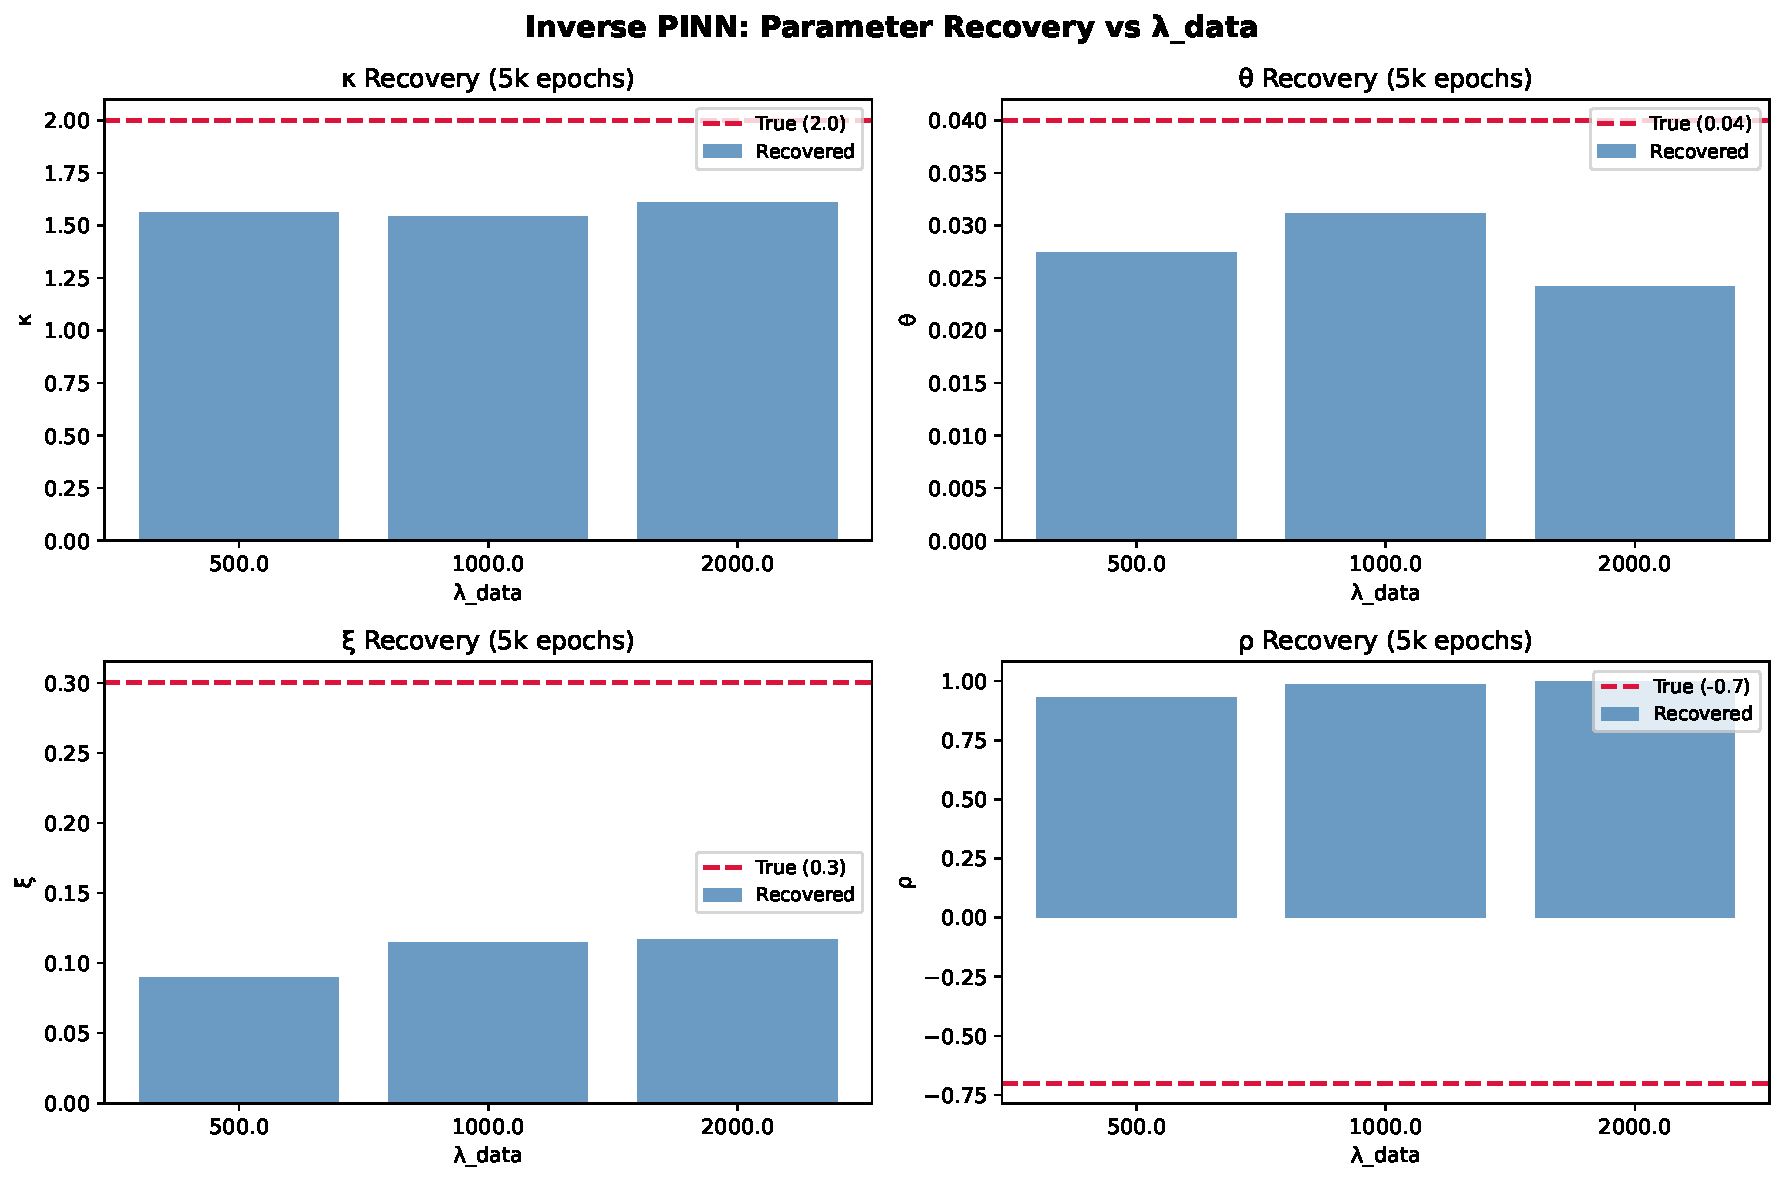
\includegraphics[width=\linewidth]{figures/hyper_inv_param_recovery.pdf}
    \caption{Caption}
    \label{fig:placeholder}
\end{figure}

\begin{figure}[H]
    \centering
    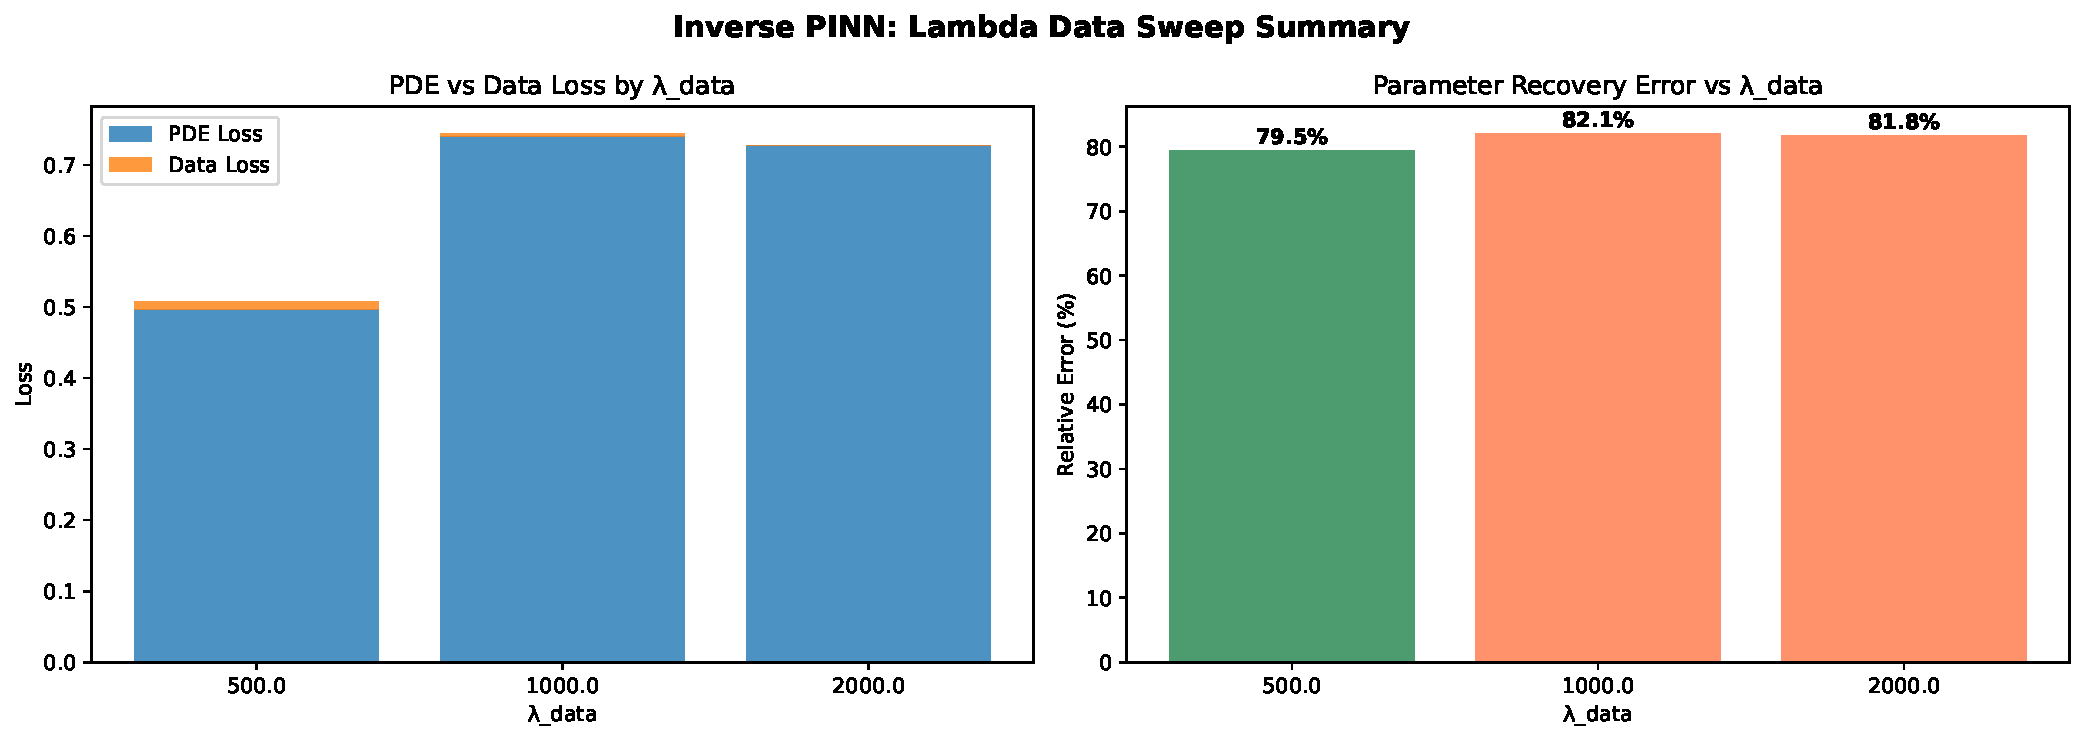
\includegraphics[width=\linewidth]{figures/hyper_inv_lambda_data_sweep.pdf}
    \caption{Caption}
    \label{fig:placeholder}
\end{figure}

\subsubsection{Inverse PINN}

\begin{figure}[H]
    \centering
    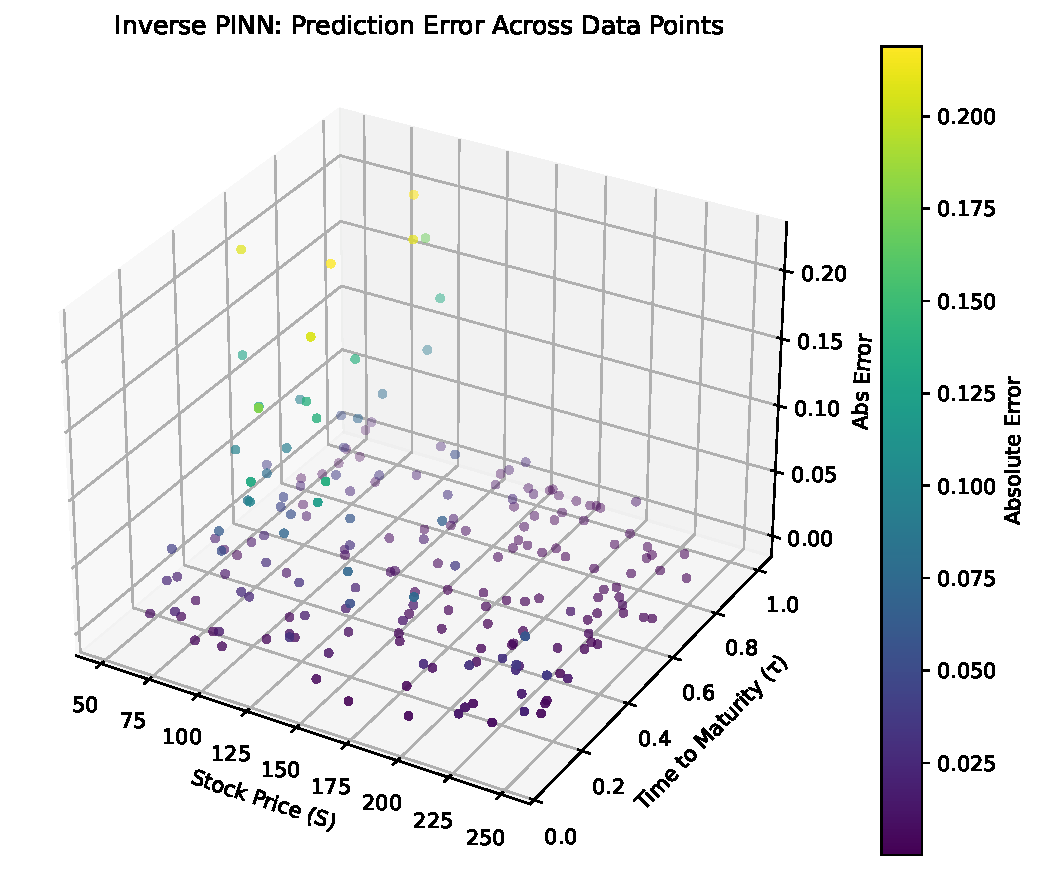
\includegraphics[width=\linewidth]{figures/pinn_error_surface.pdf}
    \caption{Caption}
    \label{fig:placeholder}
\end{figure}

\section{Conclusion}\label{section:conclusion}

This project investigated Physics-Informed Neural Networks (PINNs) as mesh-free solvers for option-pricing partial differential equations, exploiting the well-known fact that the Black--Scholes equation reduces to a heat equation under a standard change of variables and is therefore a natural target for the smooth, differentiable surrogates that PINNs produce. The work proceeded along three connected stages: a forward solver for the Black--Scholes equation, a forward solver for the Heston stochastic-volatility PDE, and an inverse calibration in which the structural Heston parameters $\kappa$, $\theta$, $\xi$, and $\rho$ were inferred jointly with the network weights $\boldsymbol{w}$ from noisy synthetic prices. The unifying theme across the three experiments is that a single differentiable price surrogate provides both prices and Greeks ``for free'' through the same automatic-differentiation machinery used to train it \parencite{baydin2018automatic,karniadakis2021physics}, and that this machinery also admits parameter calibration without external solvers.

The Black--Scholes experiment served as a controlled benchmark with a known closed-form solution. At the at-the-money evaluation point $S=K=100$ and $\tau=0.5$, the trained PINN predicted $V_{\mathrm{PINN}}=6.927159$ against the analytical value $V_{\mathrm{BS}}=6.888729$, giving an absolute error of $0.038430$ (approximately $0.56\%$ relative) and a local PDE residual of $2.746582\times 10^{-3}$ after $50{,}000$ Adam epochs (12\,min 8\,s on a single H100). The automatically differentiated Greeks (Delta, Theta, Gamma, Charm, Speed, Color) were qualitatively consistent with the analytical behavior of an at-the-money call. For a problem with a closed-form solution, the value of the PINN approach is methodological rather than computational: the closed form is faster and more accurate, but the same machinery extends seamlessly to models without closed forms or to settings where Greeks across a full surface are needed without finite-difference approximations.

The Heston experiment extended the same architecture to a three-dimensional problem $(S, v, \tau)$ governed by a PDE containing a mixed second derivative $\rho \xi v S \partial^2 V/\partial S\partial v$ and a variance-dynamics drift. Boundary conditions were imposed on both $S=0$ and $S=S_{\max}$ (with $V(S_{\max}, v, \tau)\approx S_{\max}-Ke^{-r_r\tau}$), and the network was trained for $50{,}000$ epochs (24\,min 40\,s on an A100). On the variance slice $v=v_0=0.04$ at $S=K=100$, $\tau=0.5$, the PINN predicted $V_{\mathrm{PINN}}=6.806941$ against the semi-analytical Heston value $V_{\mathrm{Heston}}=6.837137$, an absolute error of $0.030196$ (approximately $0.44\%$). However, the local PDE residual was substantially larger in magnitude ($-1.790738\times 10^{-1}$) and the loss history was visibly less stable than in the Black--Scholes case, consistent with the by-now standard observation that PINN optimization landscapes degrade as the PDE becomes stiffer, more multi-scale, or more strongly coupled \parencite{wang2021understanding,wang2022expert,krishnapriyan2021characterizing}.

The inverse experiment recast the Heston PINN as a calibration engine: the four structural parameters $(\kappa, \theta, \xi, \rho)$ were promoted to trainable variables and optimized jointly with $\boldsymbol{w}$ against $200$ noisy synthetic prices, using a two-stage schedule of $25{,}000$ Adam epochs followed by $5{,}000$ L-BFGS iterations (30{,}000 total, 16\,min 17\,s) under loss weights $\lambda_{\mathrm{PDE}}=20$, $\lambda_{\mathrm{IC}}=10$, $\lambda_{\mathrm{BC}}=5$, $\lambda_{\mathrm{data}}=1000$, and a Feller-penalty weight $\lambda_{\mathrm{Feller}}=0.1$. Judged purely on its ability to reproduce observed prices, the model performed extremely well: the final mean absolute pricing error on the $200$ synthetic observations was $0.028566$, the maximum absolute error was $0.218854$, the median relative error was approximately $0.02\%$, and the parity-plot diagnostic gave $R^2 = 0.999999$. By any pricing yardstick the calibration succeeded.

By any \emph{parameter-recovery} yardstick, however, the same calibration failed. The final recovered parameter vector was $(\kappa, \theta, \xi, \rho) = (1.588,\, 0.0266,\, 0.104,\, 0.994)$, against the true data-generating values $(2.0,\, 0.04,\, 0.3,\, -0.7)$. The most striking discrepancy is the correlation: $\rho$ converged to a strongly positive value despite the data being generated with $\rho=-0.7$, the standard equity-market sign. Mechanistically this is not surprising. The parameter $\rho$ enters the Heston PDE only through the cross term $\rho\xi v S \partial^2 V/\partial S\partial v$, and therefore appears in the data only through the implied-volatility skew that this cross term produces; with $200$ noisy points sparsely scattered across a wide $(S,v,\tau)$ region, the skew signal is far too weak to identify $\rho$ from prices alone. Moreover, the product $\xi\rho$ is more identifiable than $\rho$ individually, and even that product is recovered with the wrong sign here: $\xi\rho \approx (0.104)(0.994)\approx 0.10$ recovered against $(0.3)(-0.7)\approx -0.21$ true. This is not a simple sign confusion in $\rho$ alone but rather points to genuine multi-modality in the data-likelihood landscape, in which the optimizer found a price-consistent representation of the observations through a different combination of $\xi$ and $\rho$.

The financial implications of this two-sided result are concrete. First, forward PINNs are already useful: once trained, the network is a fast, differentiable pricing surrogate that delivers prices and a full surface of Greeks through automatic differentiation, which is directly applicable to pricing and hedging workflows. Second, inverse PINN calibration is a promising direction but is not yet competitive with classical calibration as a black-box parameter-recovery tool. Third, the data deficit identified here is much less severe in practice: real-world calibration uses listed quotes across many strikes and maturities---typically dense option chains in implied-volatility space---which is orders of magnitude richer than the $200$ points used here, and it is precisely that density (especially near-the-money skew) that classical calibration exploits to identify $\rho$. Fourth, PINNs are likely to be most valuable in settings where classical approaches are not available, in particular rough-volatility models \parencite{gatheral2018volatility,bayer2016rough,euch2019roughheston}, for which no easily-invertible characteristic function exists; that extension is left to future work.

Several concrete extensions follow directly from the experiments above. (i) Richer collocation and observation designs spanning a full strike--maturity surface rather than $200$ scattered prices, ideally with controlled noise levels and a near-the-money refinement to expose skew. (ii) Bayesian or regularized priors on $\rho$ and $\xi$ that encode the strong economic prior $\rho<0$ for equity underlyings, turning the under-identified calibration problem into a well-posed MAP problem. (iii) Loss functions formulated in implied-volatility space rather than price space, so that the skew signal that identifies $\rho$ is amplified relative to the level signal that dominates a price-MSE loss. (iv) Extension of the forward solver to American and exotic options, where the PINN's mesh-free property pays off most clearly because no rectangular grid exists. (v) Extension to rough Heston \parencite{euch2019roughheston} as the natural target where no closed-form characteristic function is easily inverted and where a differentiable surrogate is structurally hardest to beat.

The overall picture is that PINNs are a powerful and flexible differentiable framework for financial PDEs. Forward pricing is in good shape across both Black--Scholes and Heston, and the same machinery delivers Greeks essentially for free. Inverse calibration is genuinely harder and more delicate: a near-perfect price fit does not imply structural parameter recovery, and this project demonstrates both sides of that trade-off in a single end-to-end pipeline.

\clearpage
% \noindent\rule{\linewidth}{0.2pt}\vspace{-1em}
\printbibliography
\onecolumn
\appendix
\section{Appendix}\label{section:appendix}

%%%%%%%%%%%%%%%%%%%%%%%%%%%%%%%%%%%%%%%%%%%%%%%%%%%%%%%%%%%%%%%%%%%%%%%%%%%%
%%%%%%%%%%%%%%%%%%%%%%%%%%%%%%%%%%%%%%%%%%%%%%%%%%%%%%%%%%%%%%%%%%%%%%%%%%%%
%%%%%%%%%%%%%%%%%%%%%%%%%%%%%%%%%%%%%%%%%%%%%%%%%%%%%%%%%%%%%%%%%%%%%%%%%%%%

\subsection{Pathways}

\begin{figure}[H]
    \centering

    \begin{subfigure}[t]{0.92\linewidth}
        \centering
        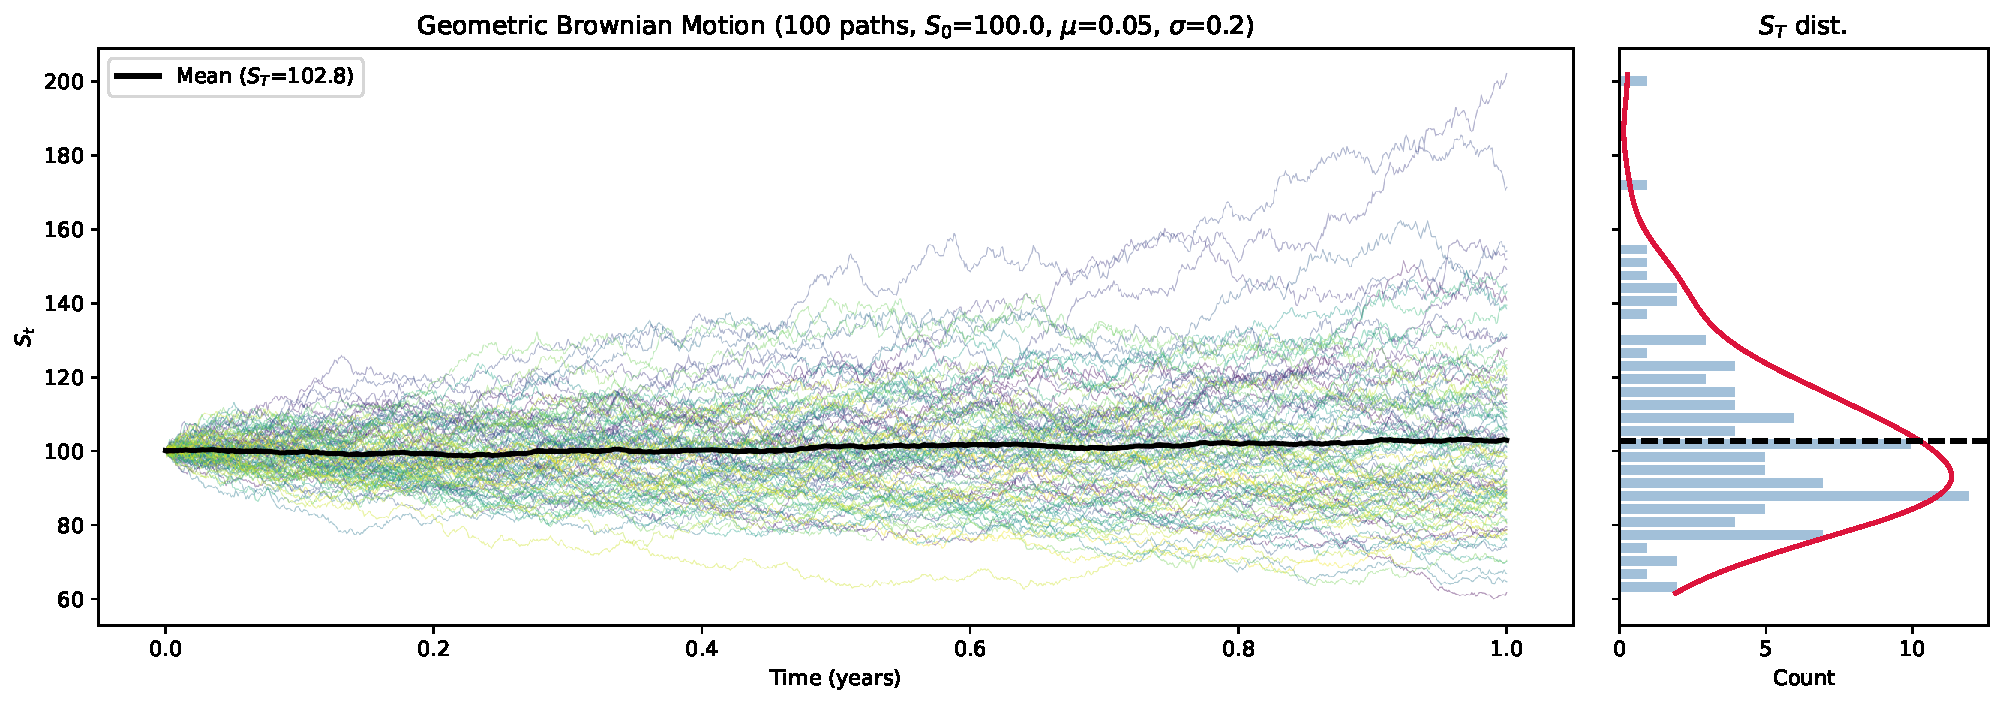
\includegraphics[width=\linewidth]{figures/brownian_path.pdf}
        \caption{Sample Brownian paths used to illustrate the stochastic driving noise in the model setup. The figure provides intuition for the random fluctuations underlying the subsequent Heston dynamics.}
        \label{fig:brownian_path.pdf}
    \end{subfigure}

    \vspace{0.55cm}

    \begin{subfigure}[t]{0.92\linewidth}
        \centering
        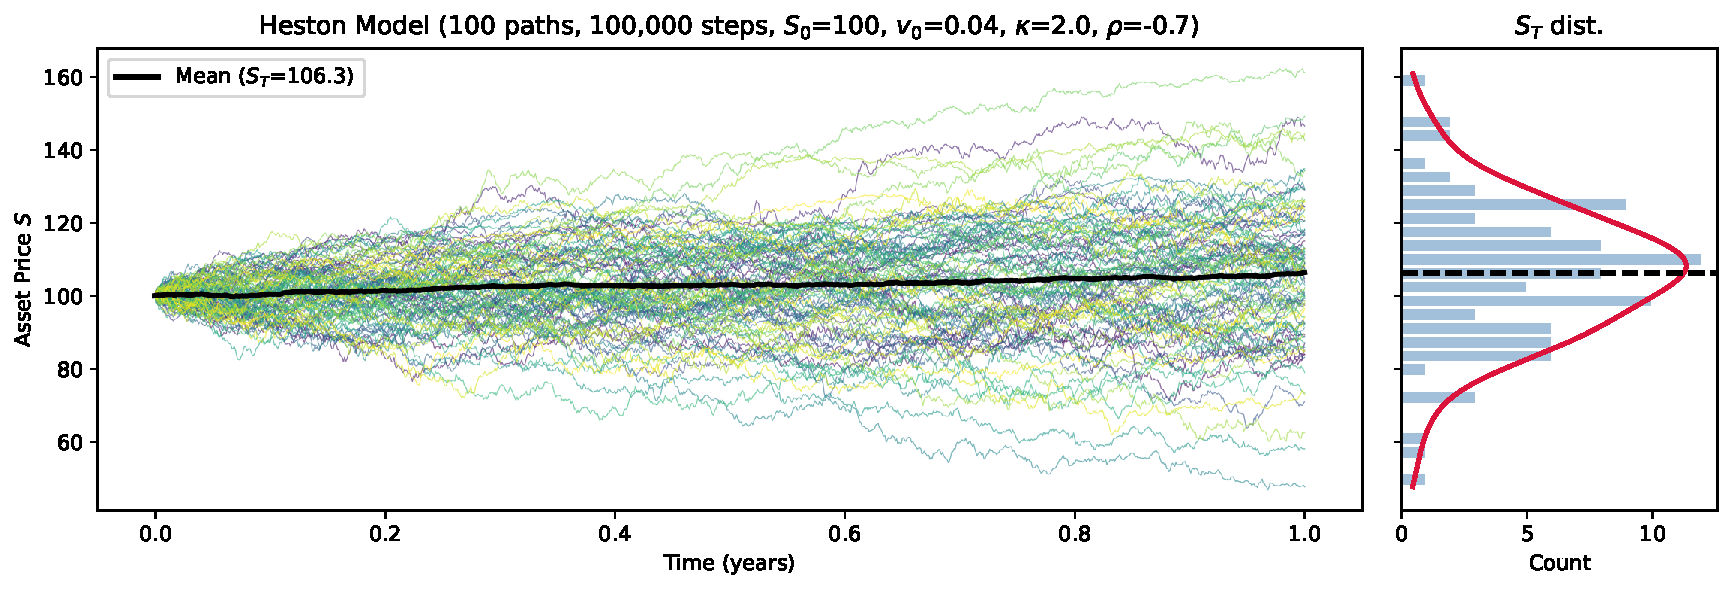
\includegraphics[width=\linewidth]{figures/heston.pdf}
        \caption{Simulated Heston price paths. The figure shows how stochastic volatility generates more realistic and irregular asset-price dynamics than constant-volatility models.}
        \label{fig:heston.pdf}
    \end{subfigure}

    \vspace{0.55cm}

    \begin{subfigure}[t]{0.92\linewidth}
        \centering
        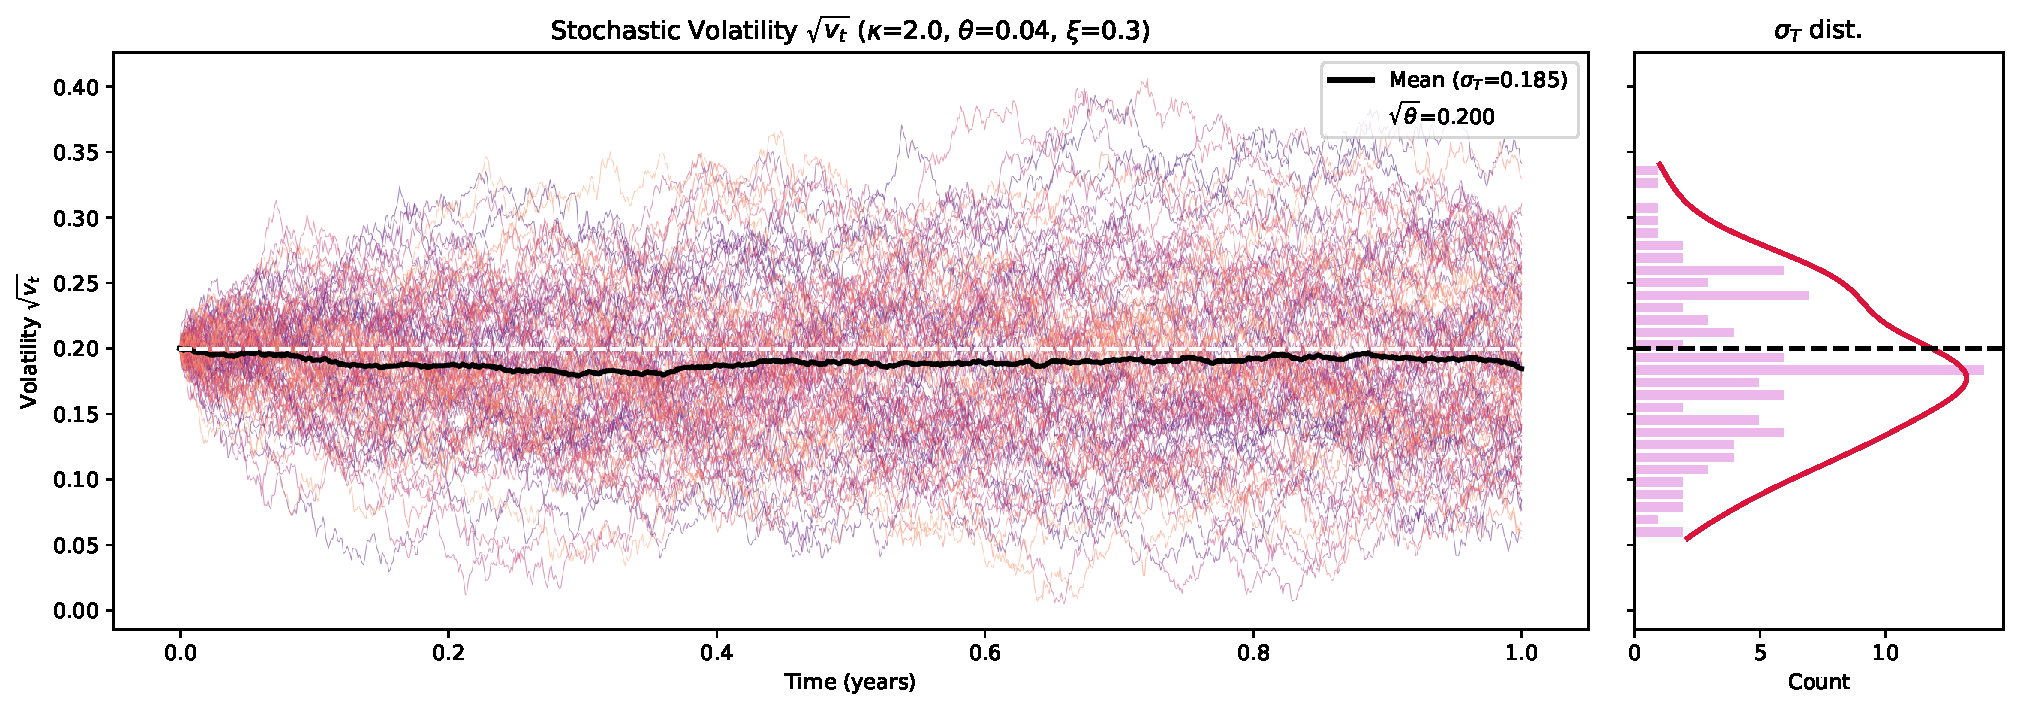
\includegraphics[width=\linewidth]{figures/heston_vol.pdf}
        \caption{Simulated Heston variance or volatility paths. The figure highlights the mean-reverting yet stochastic behavior of volatility in the Heston framework.}
        \label{fig:heston_vol.pdf}
    \end{subfigure}

    \caption{Illustration of the stochastic processes underlying the Heston model. The three panels show Brownian motion, simulated asset-price dynamics, and simulated variance dynamics in a single vertical layout.}
    \label{fig:heston_process_panel}
\end{figure}

%%%%%%%%%%%%%%%%%%%%%%%%%%%%%%%%%%%%%%%%%%%%%%%%%%%%%%%%%%%%%%%%%%%%%%%%%%%%
%%%%%%%%%%%%%%%%%%%%%%%%%%%%%%%%%%%%%%%%%%%%%%%%%%%%%%%%%%%%%%%%%%%%%%%%%%%%
%%%%%%%%%%%%%%%%%%%%%%%%%%%%%%%%%%%%%%%%%%%%%%%%%%%%%%%%%%%%%%%%%%%%%%%%%%%%



\clearpage\subsection{Training duration}

\begin{table}[H]
    \centering
    \begin{minipage}[t]{0.48\linewidth}
        \centering
        \footnotesize
        \setlength{\tabcolsep}{3pt}
        \renewcommand{\arraystretch}{1.2}
        \caption{Black--Scholes PINN training-loss history.}
        \label{tab:bs_training_loss_history}
        \begin{tabular}{rrrrr}
            \hline
            \textbf{Epoch} & \textbf{Total} & \textbf{PDE} & \textbf{IC} & \textbf{BC} \\
            \hline
                 0 & $21994.2520$ & $0.04019$ & $4398.7573$ & $0.01269$ \\
              2500 & $4.31051$    & $0.07313$ & $0.70893$   & $0.00692$ \\
              5000 & $1.17099$    & $0.04505$ & $0.14089$   & $0.00320$ \\
              7500 & $0.83849$    & $0.04067$ & $0.08446$   & $0.00189$ \\
             10000 & $0.77996$    & $0.04238$ & $0.07012$   & $0.00113$ \\
             12500 & $0.63270$    & $0.03394$ & $0.05784$   & $0.00082$ \\
             15000 & $0.44972$    & $0.02157$ & $0.04581$   & $0.00100$ \\
             17500 & $0.44924$    & $0.02296$ & $0.04332$   & $0.00060$ \\
             20000 & $0.41018$    & $0.02141$ & $0.03868$   & $0.00054$ \\
             22500 & $0.31794$    & $0.01427$ & $0.03457$   & $0.00049$ \\
             25000 & $0.26285$    & $0.01070$ & $0.03056$   & $0.00061$ \\
             27500 & $0.21871$    & $0.00805$ & $0.02712$   & $0.00052$ \\
             30000 & $0.19578$    & $0.00702$ & $0.02470$   & $0.00041$ \\
             32500 & $0.17387$    & $0.00561$ & $0.02314$   & $0.00042$ \\
             35000 & $0.15051$    & $0.00394$ & $0.02187$   & $0.00035$ \\
             37500 & $0.13306$    & $0.00286$ & $0.02053$   & $0.00036$ \\
             40000 & $0.13759$    & $0.00390$ & $0.01940$   & $0.00032$ \\
             42500 & $0.11622$    & $0.00228$ & $0.01837$   & $0.00031$ \\
             45000 & $0.11086$    & $0.00220$ & $0.01748$   & $0.00029$ \\
             47500 & $0.10621$    & $0.00212$ & $0.01674$   & $0.00027$ \\
            \hline
        \end{tabular}
    \end{minipage}\hfill
    \begin{minipage}[t]{0.48\linewidth}
        \centering
        \footnotesize
        \setlength{\tabcolsep}{3pt}
        \renewcommand{\arraystretch}{1.2}
        \caption{Heston PINN training-loss history.}
        \label{tab:heston_training_loss_history}
        \begin{tabular}{rrrrr}
            \hline
            \textbf{Epoch} & \textbf{Total} & \textbf{PDE} & \textbf{IC} & \textbf{BC} \\
            \hline
                 0 & $46860.6875$ & $0.03398$  & $4686.0298$ & $0.01044$ \\
              2500 & $137.51643$  & $9.55106$  & $3.99954$   & $0.40209$ \\
              5000 & $125.37741$  & $5.42175$  & $7.08815$   & $0.05568$ \\
              7500 & $58.41161$   & $1.91550$  & $3.91287$   & $0.02558$ \\
             10000 & $202.79363$  & $17.57729$ & $2.69334$   & $0.01747$ \\
             12500 & $266.89291$  & $21.35045$ & $5.33818$   & $0.00133$ \\
             15000 & $50.37729$   & $4.27836$  & $0.75459$   & $0.00957$ \\
             17500 & $47.02234$   & $2.73344$  & $1.95774$   & $0.02211$ \\
             20000 & $35.66247$   & $1.98122$  & $1.57846$   & $0.01313$ \\
             22500 & $18.46533$   & $1.19200$  & $0.65409$   & $0.00090$ \\
             25000 & $10.65871$   & $0.89655$  & $0.16848$   & $0.00168$ \\
             27500 & $7.28630$    & $0.35398$  & $0.37364$   & $0.00202$ \\
             30000 & $5.99006$    & $0.27701$  & $0.32107$   & $0.00186$ \\
             32500 & $2.35999$    & $0.13831$  & $0.09759$   & $0.00020$ \\
             35000 & $1.87818$    & $0.09468$  & $0.09288$   & $0.00052$ \\
             37500 & $1.40915$    & $0.06286$  & $0.07782$   & $0.00047$ \\
             40000 & $1.19361$    & $0.05294$  & $0.06630$   & $0.00024$ \\
             42500 & $0.86779$    & $0.02564$  & $0.06107$   & $0.00015$ \\
             45000 & $0.63638$    & $0.01763$  & $0.04598$   & $0.00007$ \\
             47500 & $0.53413$    & $0.01536$  & $0.03803$   & $0.00005$ \\
            \hline
        \end{tabular}
    \end{minipage}

    \vspace{0.3cm}

    \centering
    \footnotesize
    \setlength{\tabcolsep}{2.5pt}
    \renewcommand{\arraystretch}{1.2}
    \caption{Inverse PINN training and calibration history with evolving parameter estimates $\kappa$, $\theta$, $\xi$, $\rho$.}
    \label{tab:inverse_pinn_calibration_history}
    \begin{adjustbox}{max width=\linewidth}
    \begin{tabular}{rrrrrrrrrrr}
        \hline
        \textbf{Epoch} & \textbf{Total} & \textbf{PDE} & \textbf{IC} & \textbf{BC} & \textbf{Data} & \textbf{Feller} & $\boldsymbol{\kappa}$ & $\boldsymbol{\theta}$ & $\boldsymbol{\xi}$ & $\boldsymbol{\rho}$ \\
        \hline
             0 & $5042358.0000$ & $10.725791$ & $4134.6187$ & $28.860662$ & $5000.6528$ & $0.002455$ & $0.999$ & $0.1001$ & $0.500$ & $-0.001$ \\
          1500 & $4059.0977$    & $87.752625$ & $29.4920$   & $0.367506$  & $2.0073$    & $0.000000$ & $1.620$ & $0.0422$ & $0.163$ & $0.793$ \\
          3000 & $1085.7815$    & $11.841378$ & $7.7701$    & $0.067702$  & $0.7709$    & $0.000000$ & $1.578$ & $0.0357$ & $0.133$ & $0.888$ \\
          4500 & $1028.3889$    & $5.079397$  & $3.6259$    & $0.043186$  & $0.8903$    & $0.000000$ & $1.536$ & $0.0344$ & $0.123$ & $0.921$ \\
          6000 & $283.0856$     & $5.284629$  & $2.4379$    & $0.042856$  & $0.1528$    & $0.000000$ & $1.504$ & $0.0345$ & $0.118$ & $0.940$ \\
          7500 & $1080.6104$    & $21.654047$ & $3.2561$    & $0.109399$  & $0.6144$    & $0.000000$ & $1.485$ & $0.0344$ & $0.115$ & $0.955$ \\
          9000 & $141.1073$     & $2.657735$  & $1.3538$    & $0.017838$  & $0.0743$    & $0.000000$ & $1.484$ & $0.0337$ & $0.112$ & $0.964$ \\
         10500 & $357.5637$     & $5.206030$  & $1.4301$    & $0.059183$  & $0.2388$    & $0.000000$ & $1.469$ & $0.0334$ & $0.110$ & $0.973$ \\
         12000 & $82.9516$      & $1.525354$  & $0.9522$    & $0.021463$  & $0.0428$    & $0.000000$ & $1.480$ & $0.0320$ & $0.109$ & $0.978$ \\
         13500 & $144.8452$     & $3.712763$  & $0.8913$    & $0.042495$  & $0.0615$    & $0.000000$ & $1.493$ & $0.0307$ & $0.107$ & $0.983$ \\
         15000 & $86.0975$      & $1.212989$  & $0.7499$    & $0.004642$  & $0.0543$    & $0.000000$ & $1.501$ & $0.0300$ & $0.107$ & $0.986$ \\
         16500 & $42.8948$      & $1.066067$  & $0.6579$    & $0.002672$  & $0.0150$    & $0.000000$ & $1.514$ & $0.0293$ & $0.107$ & $0.988$ \\
         18000 & $28.8773$      & $0.705716$  & $0.4965$    & $0.002691$  & $0.0098$    & $0.000000$ & $1.536$ & $0.0282$ & $0.106$ & $0.991$ \\
         19500 & $36.3960$      & $1.234485$  & $0.5088$    & $0.004252$  & $0.0066$    & $0.000000$ & $1.548$ & $0.0278$ & $0.106$ & $0.992$ \\
         21000 & $25.2769$      & $0.750561$  & $0.4207$    & $0.003757$  & $0.0060$    & $0.000000$ & $1.562$ & $0.0273$ & $0.105$ & $0.993$ \\
         22500 & $19.7579$      & $0.587920$  & $0.4024$    & $0.002703$  & $0.0040$    & $0.000000$ & $1.574$ & $0.0269$ & $0.105$ & $0.994$ \\
         24000 & $17.8799$      & $0.548446$  & $0.3758$    & $0.002470$  & $0.0031$    & $0.000000$ & $1.584$ & $0.0267$ & $0.105$ & $0.994$ \\
         25500 & $17.3094$      & $0.533012$  & $0.3654$    & $0.002380$  & $0.0030$    & $0.000000$ & $1.588$ & $0.0266$ & $0.104$ & $0.994$ \\
         27000 & $17.3094$      & $0.533012$  & $0.3654$    & $0.002380$  & $0.0030$    & $0.000000$ & $1.588$ & $0.0266$ & $0.104$ & $0.994$ \\
         28500 & $17.3094$      & $0.533012$  & $0.3654$    & $0.002380$  & $0.0030$    & $0.000000$ & $1.588$ & $0.0266$ & $0.104$ & $0.994$ \\
         29999 & $17.3094$      & $0.533012$  & $0.3654$    & $0.002380$  & $0.0030$    & $0.000000$ & $1.588$ & $0.0266$ & $0.104$ & $0.994$ \\
        \hline
    \end{tabular}
    \end{adjustbox}
\end{table}

\vspace{-0.15cm}

\noindent\footnotesize
\textbf{Notes for Tables~\ref{tab:bs_training_loss_history}--\ref{tab:inverse_pinn_calibration_history}.}
\textbf{(BS)} 50000 epochs in 12\,min 8\,s; 6250 points (5000 interior, 1000 IC, 250 BC); final total loss $0.102625$.
\textbf{(Heston)} 50000 epochs in 9\,min 7\,s; 12250 points (10000 interior, 2000 IC, 250 BC); final total loss $0.485010$.
\textbf{(Inverse)} 30000 epochs in 16\,min 27\,s; final losses --- total $17.3094$, PDE $0.533012$, data $0.0030$; final calibrated $\kappa=1.588$, $\theta=0.0266$, $\xi=0.104$, $\rho=0.994$.
\normalsize

%%%%%%%%%%%%%%%%%%%%%%%%%%%%%%%%%%%%%%%%%%%%%%%%%%%%%%%%%%%%%%%%%%%%%%%%%%%%
%%%%%%%%%%%%%%%%%%%%%%%%%%%%%%%%%%%%%%%%%%%%%%%%%%%%%%%%%%%%%%%%%%%%%%%%%%%%
%%%%%%%%%%%%%%%%%%%%%%%%%%%%%%%%%%%%%%%%%%%%%%%%%%%%%%%%%%%%%%%%%%%%%%%%%%%%


\clearpage\subsection{Black-Scholes PINN}

\begin{figure}[H]
    \centering

    \begin{subfigure}[t]{0.49\linewidth}
        \centering
        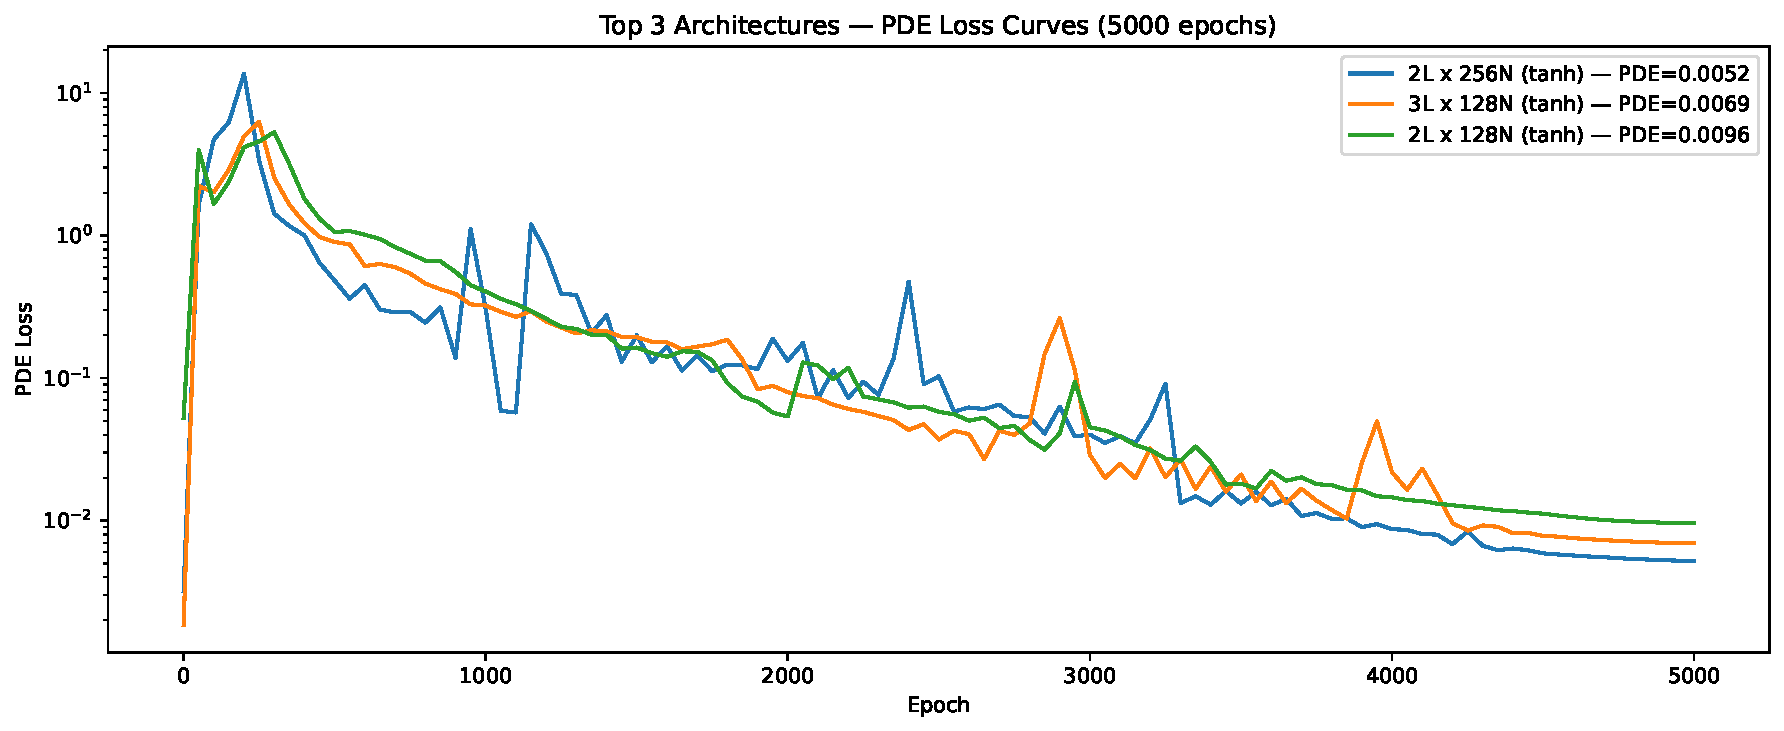
\includegraphics[width=\linewidth]{figures/hyper_bs_arch_top3_curves.pdf}
        \caption{Training curves for the three best-performing Black--Scholes architectures. The plot compares convergence speed and stability, showing whether the leading architectures differ mainly in final accuracy or in optimization dynamics.}
        \label{fig:hyper_bs_arch_top3_curves.pdf}
    \end{subfigure}
    \hfill
    \begin{subfigure}[t]{0.49\linewidth}
        \centering
        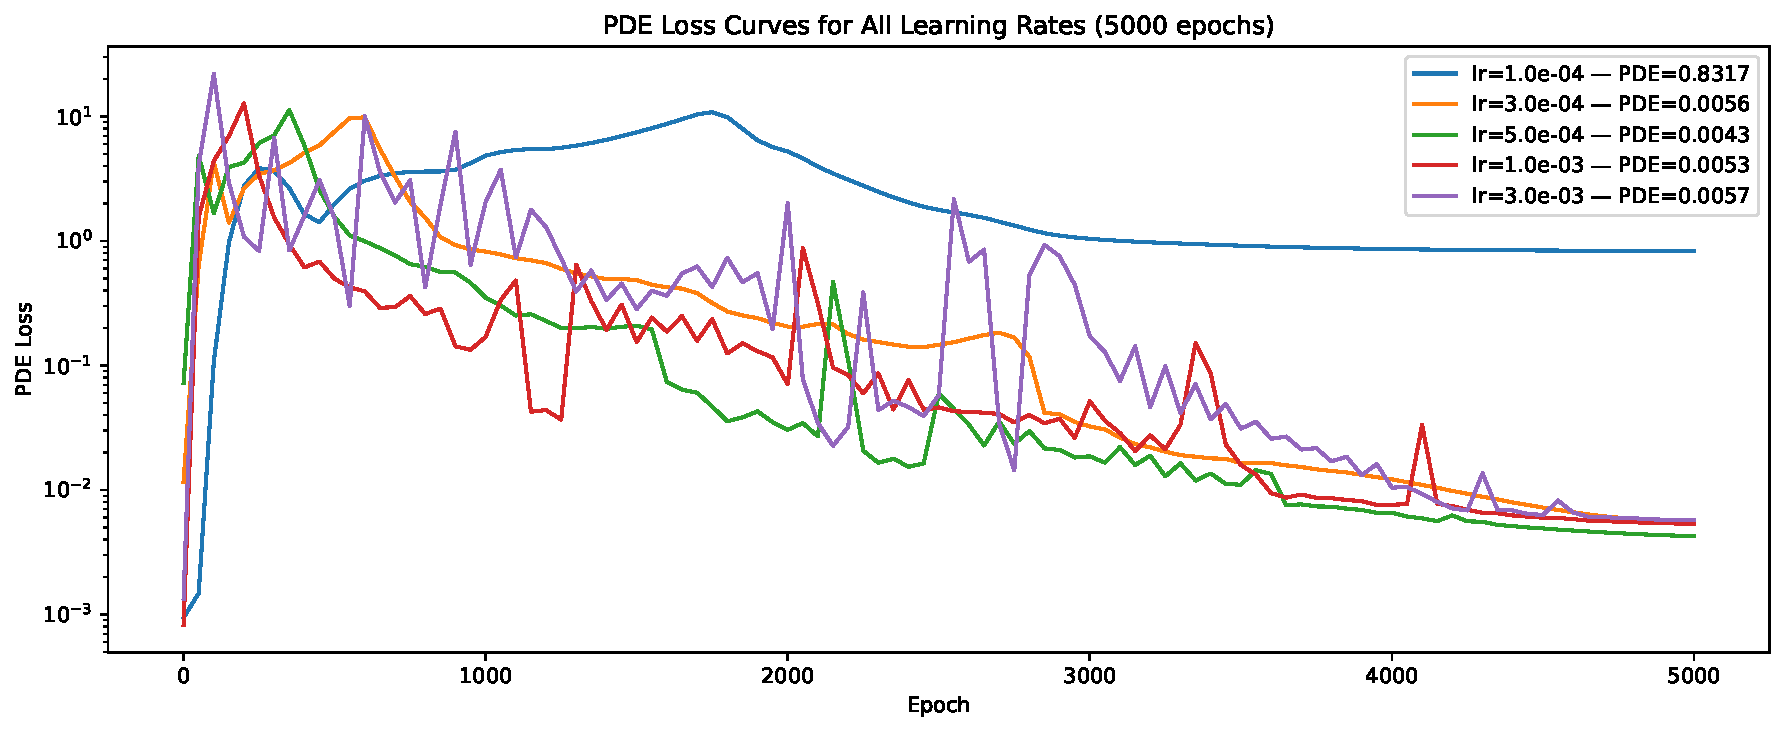
\includegraphics[width=\linewidth]{figures/hyper_bs_lr_curves.pdf}
        \caption{Training curves for the tested Black--Scholes learning rates. The figure shows how learning-rate selection affects convergence speed, oscillation, and the final loss level.}
        \label{fig:hyper_bs_lr_curves.pdf}
    \end{subfigure}

    \vspace{0.5cm}

    \begin{subfigure}[t]{0.49\linewidth}
        \centering
        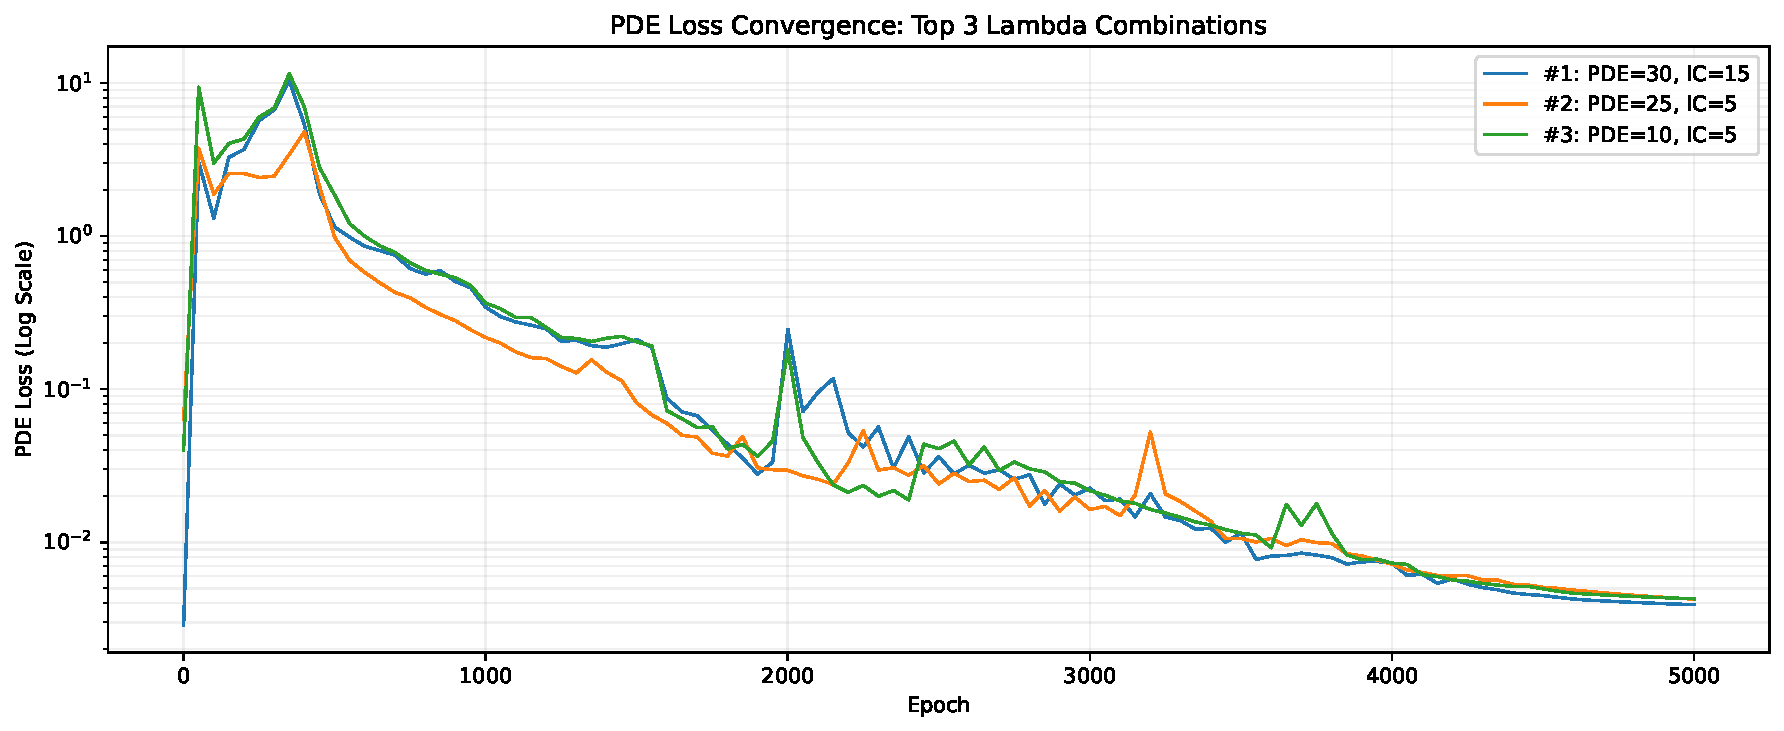
\includegraphics[width=\linewidth]{figures/hyper_bs_top3_curves.pdf}
        \caption{Training curves for the three best-performing Black--Scholes $\lambda$ configurations. The plot shows whether the strongest loss-weight choices produce consistently smooth convergence or only improve final error after longer training.}
        \label{fig:hyper_bs_top3_curves.pdf}
    \end{subfigure}
    \hfill
    \begin{subfigure}[t]{0.49\linewidth}
        \centering
        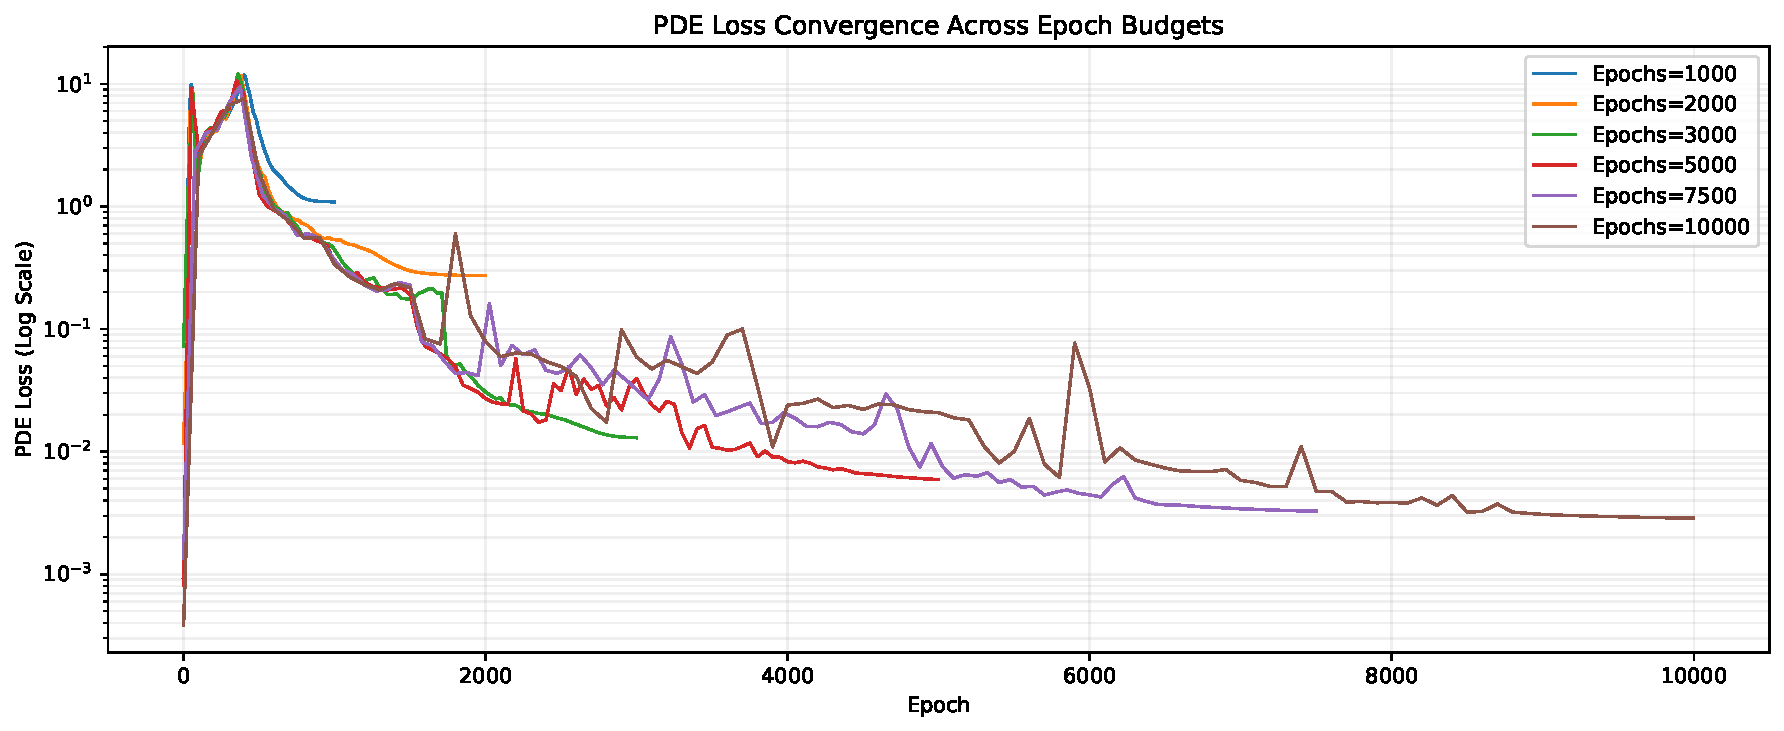
\includegraphics[width=\linewidth]{figures/hyper_bs_conv_curves.pdf}
        \caption{Training curves for the Black--Scholes convergence experiments. The figure illustrates the relationship between training duration, loss decay, and eventual stabilization of the optimization process.}
        \label{fig:hyper_bs_conv_curves.pdf}
    \end{subfigure}

    \caption{Training-curve comparison for the main Black--Scholes hyperparameter experiments. The four panels summarize the effects of architecture choice, learning rate, loss-weight selection, and training duration on convergence behavior.}
    \label{fig:hyper_bs_curves_panel}
\end{figure}

\begin{figure}[H]
    \centering

    \begin{subfigure}[t]{0.49\linewidth}
        \centering
        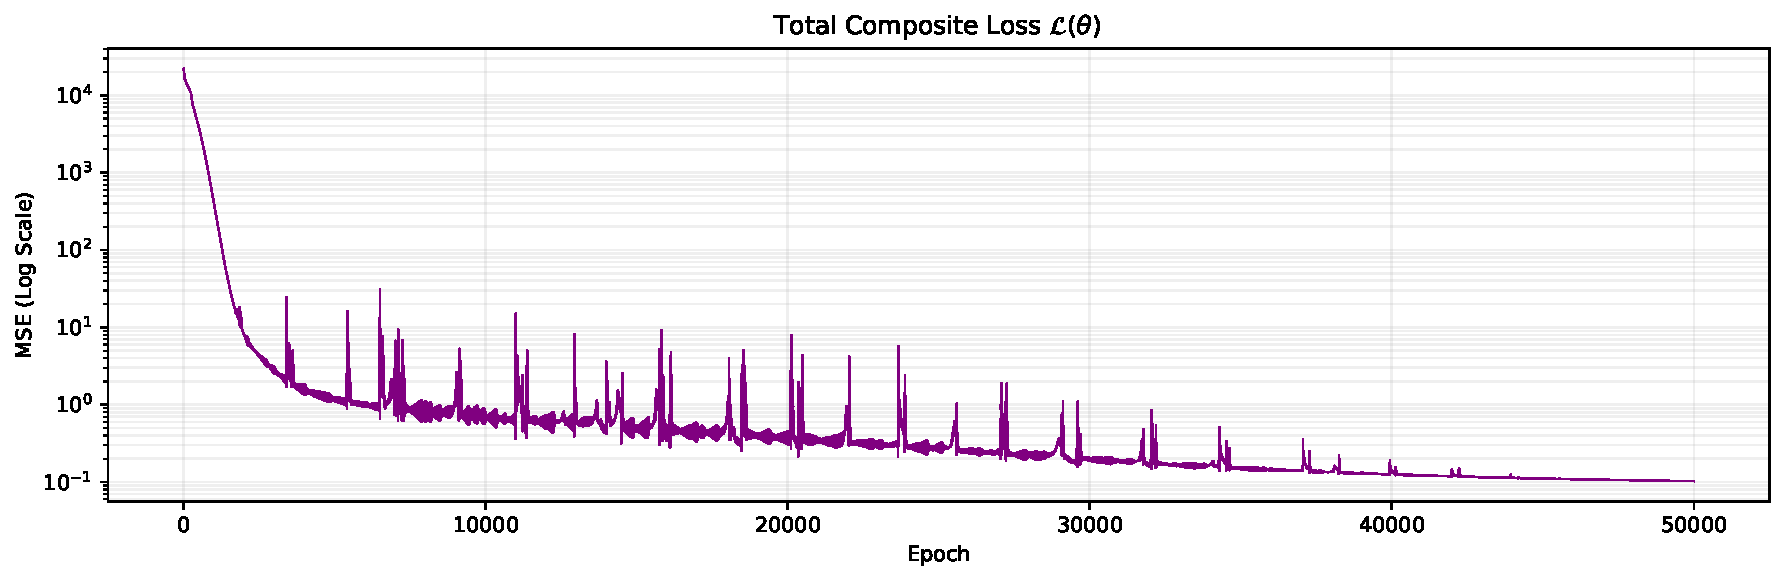
\includegraphics[width=\linewidth]{figures/pinn_bs_loss_total.pdf}
        \caption{Total training loss for the final Black--Scholes PINN. This curve summarizes the overall optimization objective across the full training run.}
        \label{fig:pinn_bs_loss_total.pdf}
    \end{subfigure}
    \hfill
    \begin{subfigure}[t]{0.49\linewidth}
        \centering
        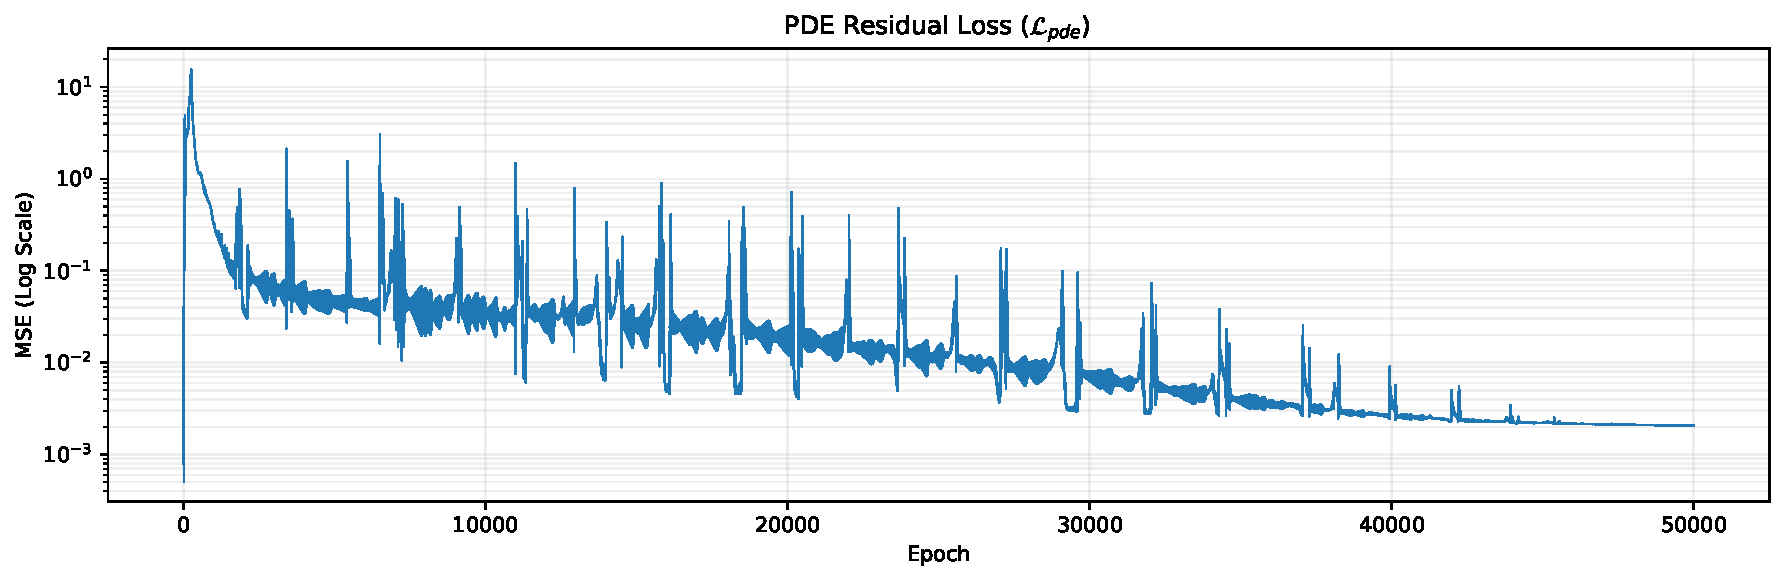
\includegraphics[width=\linewidth]{figures/pinn_bs_loss_pde.pdf}
        \caption{PDE-residual loss for the final Black--Scholes PINN. This component measures how well the learned solution satisfies the Black--Scholes equation in the interior domain.}
        \label{fig:pinn_bs_loss_pde.pdf}
    \end{subfigure}

    \vspace{0.6cm}

    \begin{subfigure}[t]{0.49\linewidth}
        \centering
        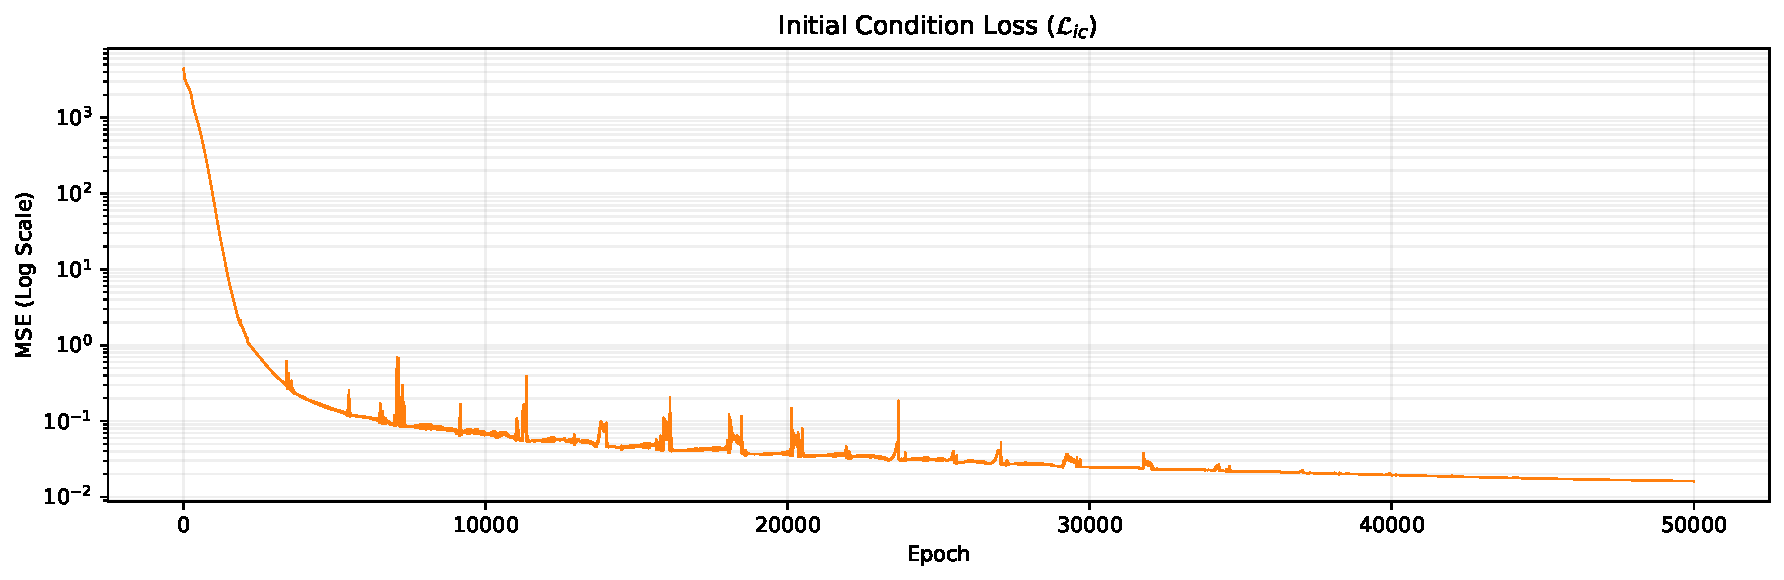
\includegraphics[width=\linewidth]{figures/pinn_bs_loss_ic.pdf}
        \caption{Initial-condition loss for the final Black--Scholes PINN. This term tracks how accurately the payoff condition at maturity is enforced during training.}
        \label{fig:pinn_bs_loss_ic.pdf}
    \end{subfigure}
    \hfill
    \begin{subfigure}[t]{0.49\linewidth}
        \centering
        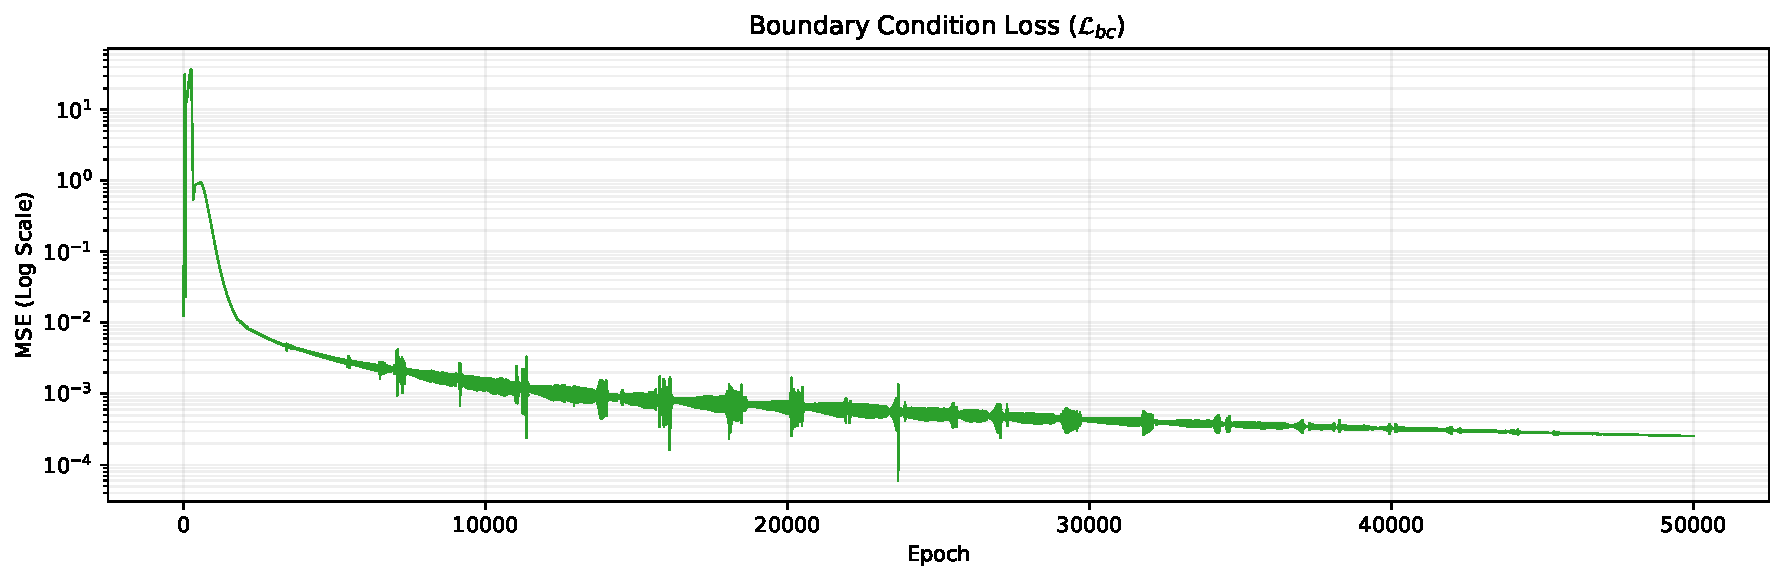
\includegraphics[width=\linewidth]{figures/pinn_bs_loss_bc.pdf}
        \caption{Boundary-condition loss for the final Black--Scholes PINN. This curve shows how well the network respects the imposed boundary behavior at the edges of the spatial domain.}
        \label{fig:pinn_bs_loss_bc.pdf}
    \end{subfigure}

    \caption{Loss decomposition for the final Black--Scholes PINN. The four panels show the evolution of the total, PDE, initial-condition, and boundary-condition losses, providing a compact overview of convergence throughout training.}
    \label{fig:pinn_bs_loss_panel}
\end{figure}

%%%%%%%%%%%%%%%%%%%%%%%%%%%%%%%%%%%%%%%%%%%%%%%%%%%%%%%%%%%%%%%%%%%%%%%%%%%%
%%%%%%%%%%%%%%%%%%%%%%%%%%%%%%%%%%%%%%%%%%%%%%%%%%%%%%%%%%%%%%%%%%%%%%%%%%%%
%%%%%%%%%%%%%%%%%%%%%%%%%%%%%%%%%%%%%%%%%%%%%%%%%%%%%%%%%%%%%%%%%%%%%%%%%%%%

\clearpage\subsection{Heston PINN}

\begin{figure}[H]
    \centering

    \begin{subfigure}[t]{0.49\linewidth}
        \centering
        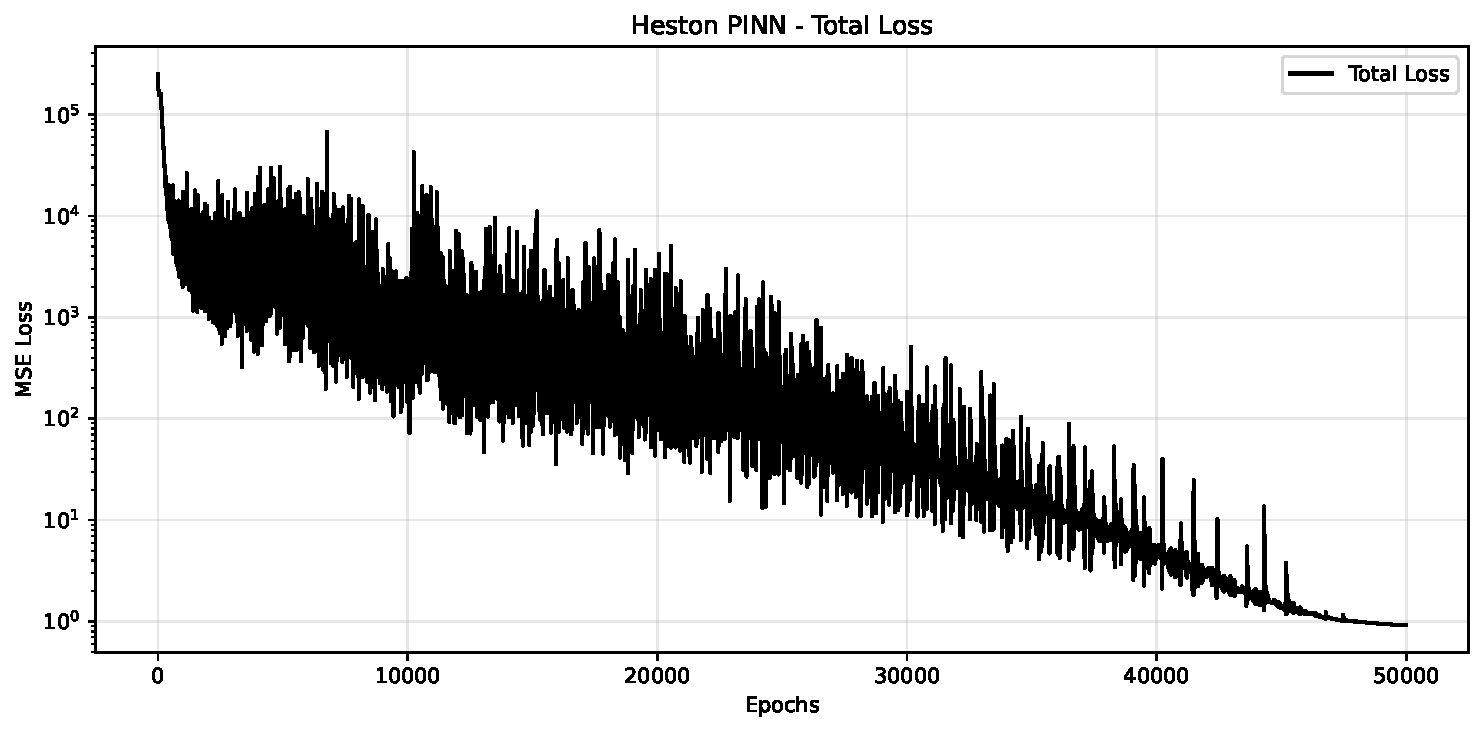
\includegraphics[width=\linewidth]{figures/pinn_hs_loss_total.pdf}
        \caption{Total training loss for the Heston PINN. This curve summarizes the overall optimization objective during training.}
        \label{fig:pinn_hs_loss_total.pdf}
    \end{subfigure}
    \hfill
    \begin{subfigure}[t]{0.49\linewidth}
        \centering
        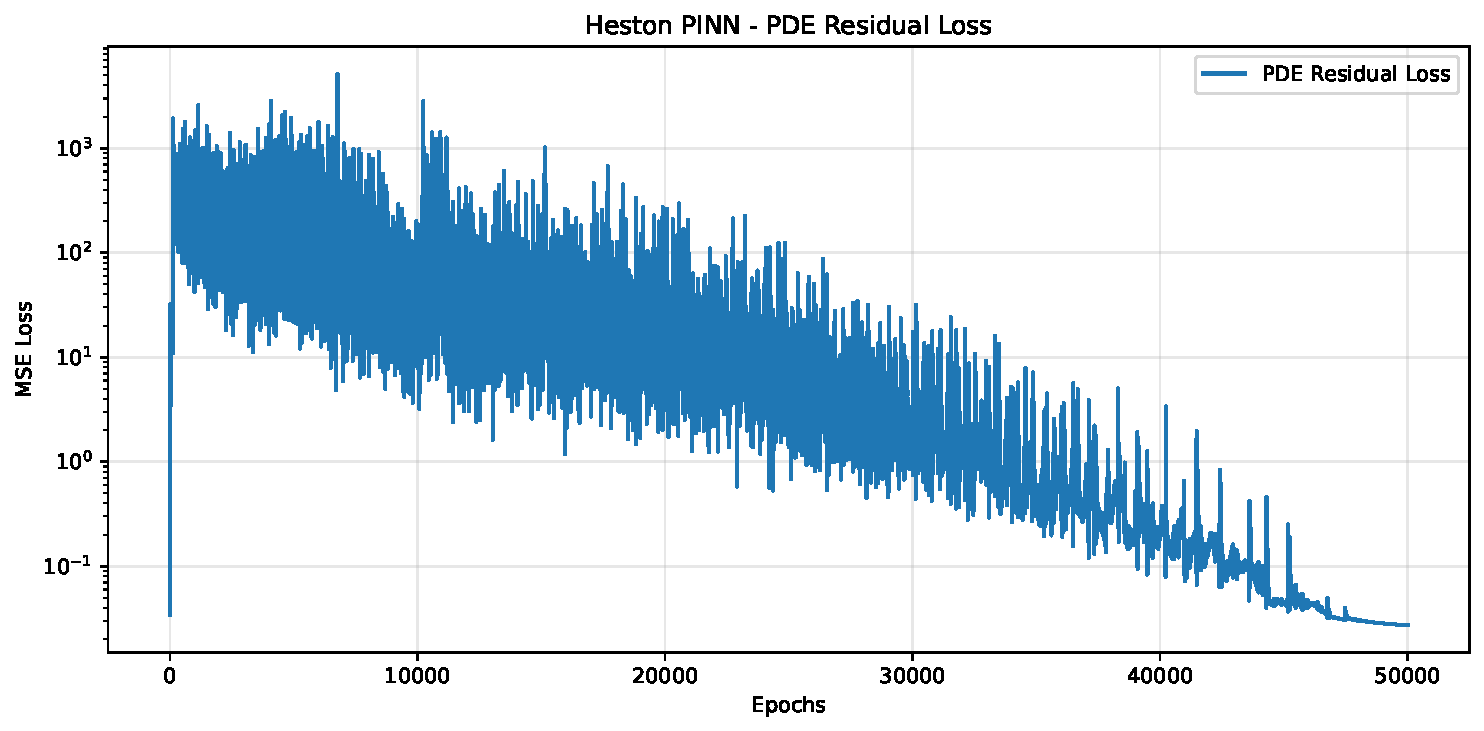
\includegraphics[width=\linewidth]{figures/pinn_hs_loss_pde.pdf}
        \caption{PDE-residual loss for the Heston PINN. This component tracks how well the learned solution satisfies the Heston equation in the interior domain.}
        \label{fig:pinn_hs_loss_pde.pdf}
    \end{subfigure}

    \vspace{0.6cm}

    \begin{subfigure}[t]{0.49\linewidth}
        \centering
        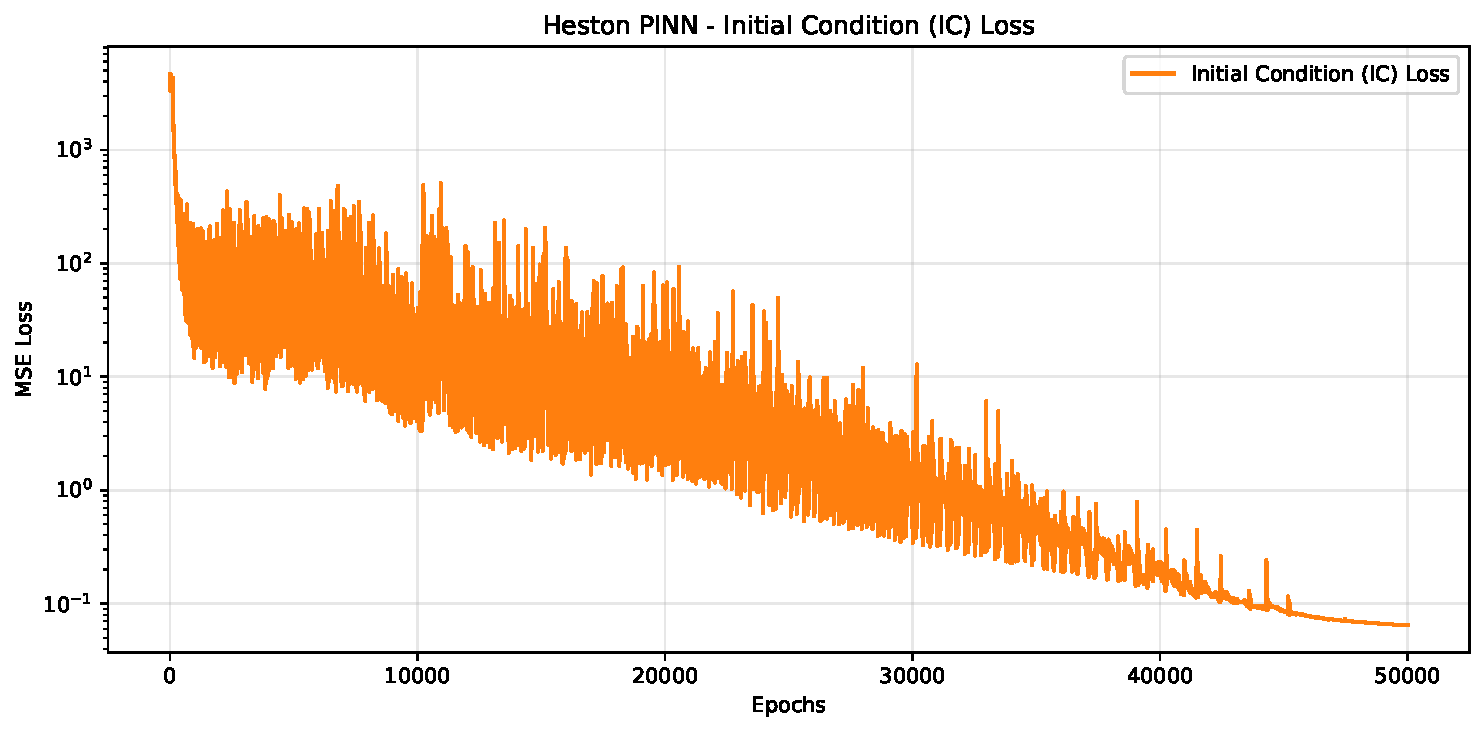
\includegraphics[width=\linewidth]{figures/pinn_hs_loss_ic.pdf}
        \caption{Initial-condition loss for the Heston PINN. This measures how accurately the terminal payoff condition is enforced.}
        \label{fig:pinn_hs_loss_ic.pdf}
    \end{subfigure}
    \hfill
    \begin{subfigure}[t]{0.49\linewidth}
        \centering
        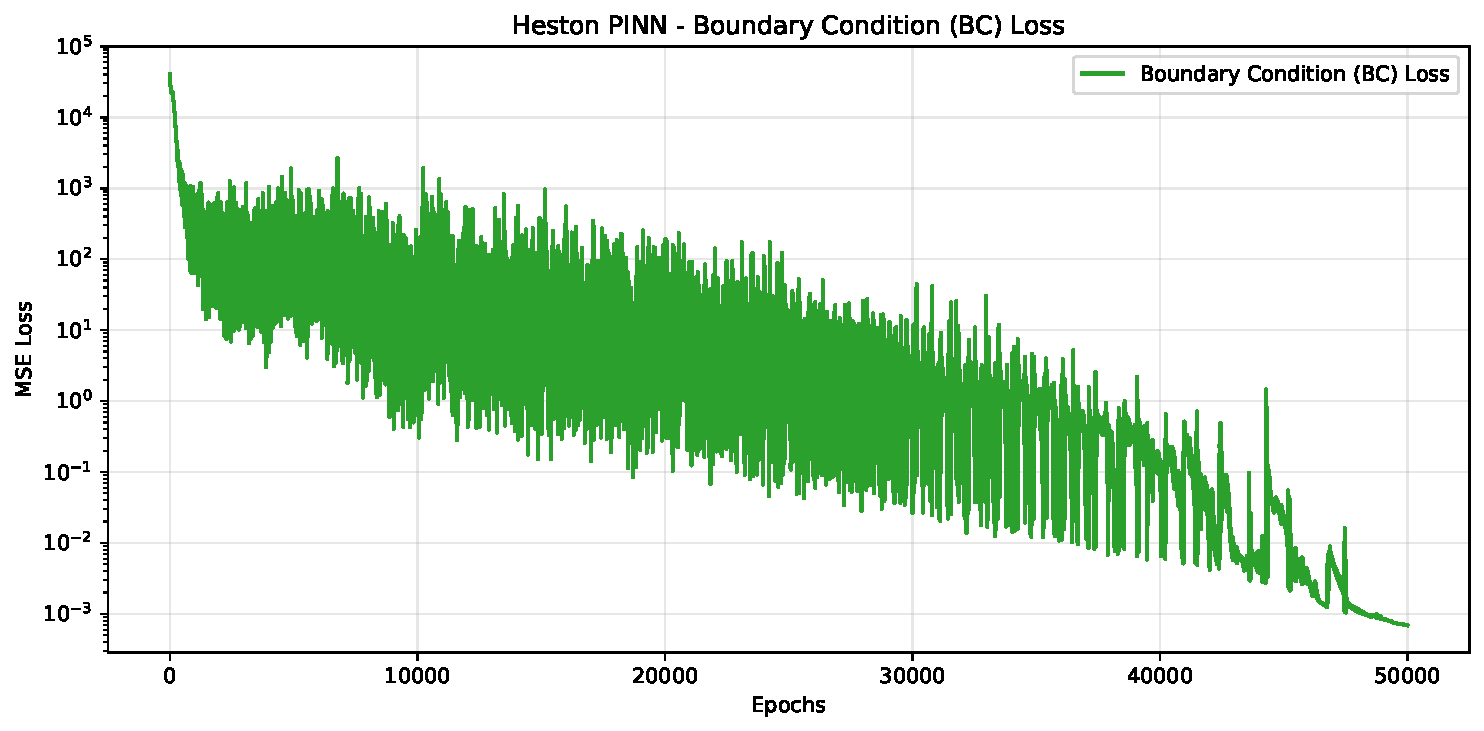
\includegraphics[width=\linewidth]{figures/pinn_hs_loss_bc.pdf}
        \caption{Boundary-condition loss for the Heston PINN. This component shows how well the model respects the imposed boundary behavior during training.}
        \label{fig:pinn_hs_loss_bc.pdf}
    \end{subfigure}

    \caption{Loss decomposition for the final Heston PINN. The four panels show the evolution of the total, PDE, initial-condition, and boundary-condition losses, providing a compact overview of convergence behavior across the full training run.}
    \label{fig:pinn_hs_loss_panel}
\end{figure}


%%%%%%%%%%%%%%%%%%%%%%%%%%%%%%%%%%%%%%%%%%%%%%%%%%%%%%%%%%%%%%%%%%%%%%%%%%%%
%%%%%%%%%%%%%%%%%%%%%%%%%%%%%%%%%%%%%%%%%%%%%%%%%%%%%%%%%%%%%%%%%%%%%%%%%%%%
%%%%%%%%%%%%%%%%%%%%%%%%%%%%%%%%%%%%%%%%%%%%%%%%%%%%%%%%%%%%%%%%%%%%%%%%%%%%


\clearpage\subsection{Inverse PINN}

\begin{figure}[H]
    \centering

    \begin{subfigure}[t]{0.8\linewidth}
        \centering
        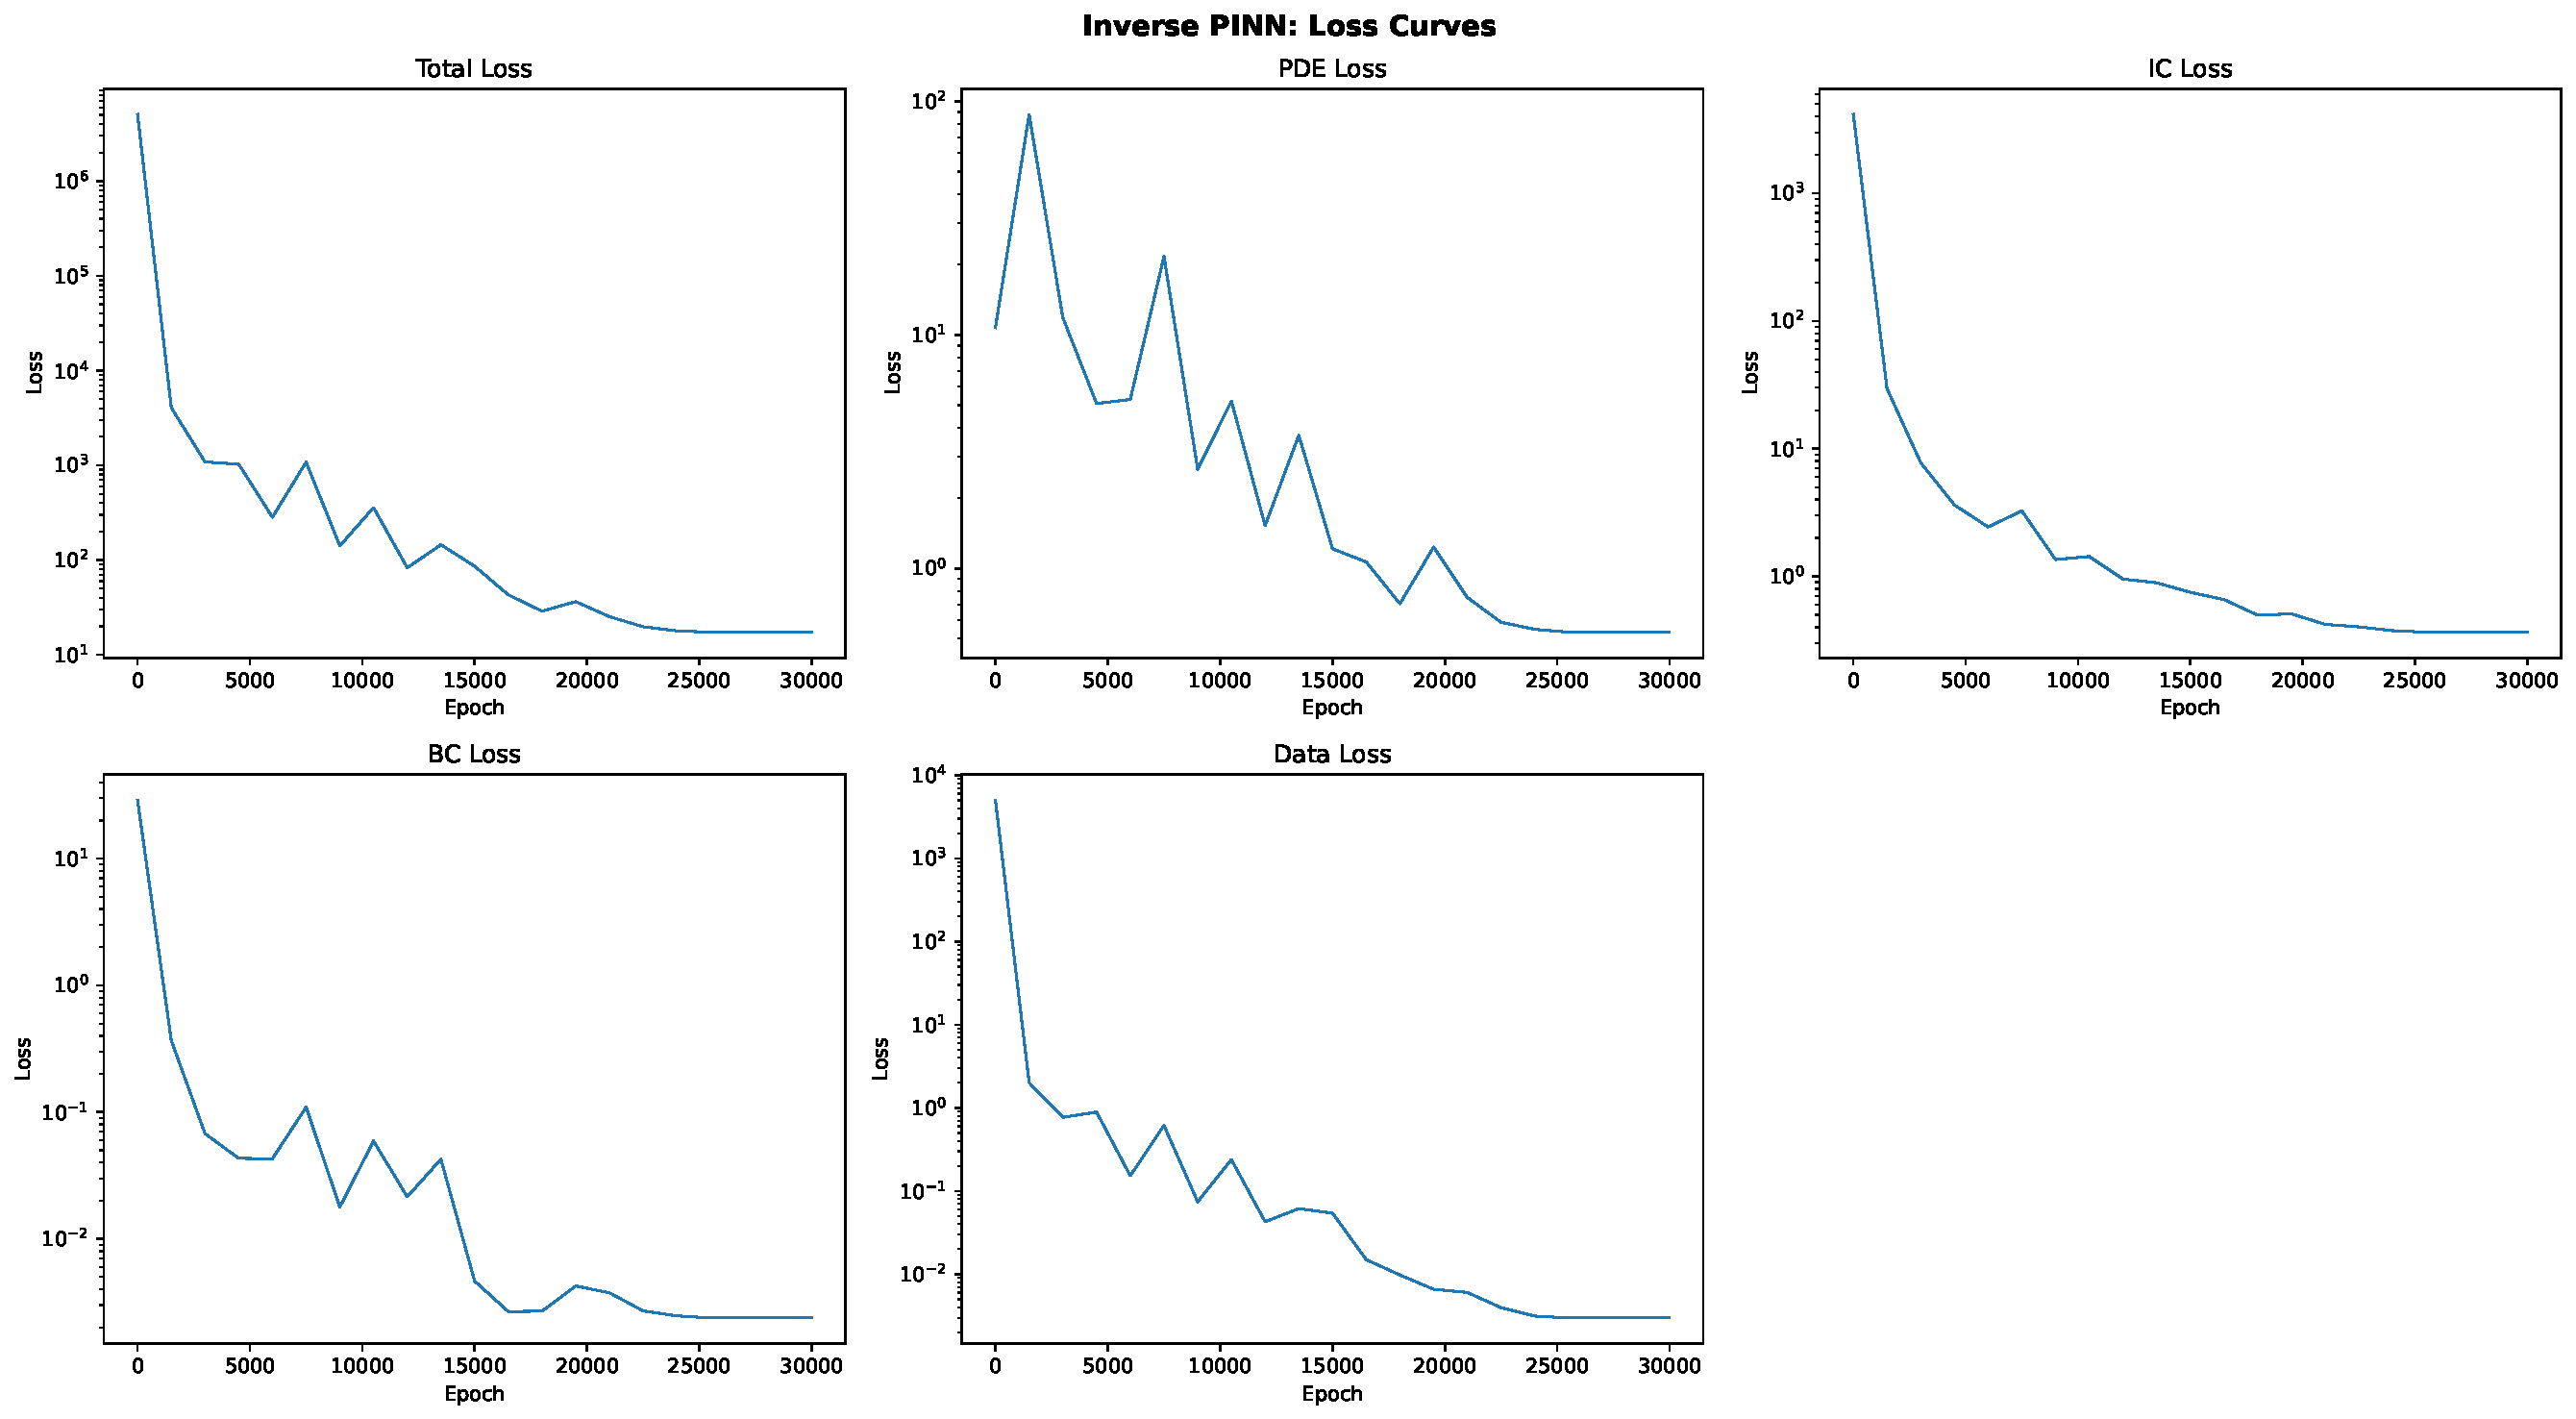
\includegraphics[width=\linewidth]{figures/pinn_inv_losses.pdf}
        \caption{Loss decomposition for the inverse PINN calibration. The figure tracks the optimization objective and its constituent terms, showing how the model balances PDE consistency, boundary and initial conditions, market-data fit, and regularization during training.}
        \label{fig:pinn_inv_losses.pdf}
    \end{subfigure}

    \vspace{0.55cm}

    \begin{subfigure}[t]{0.8\linewidth}
        \centering
        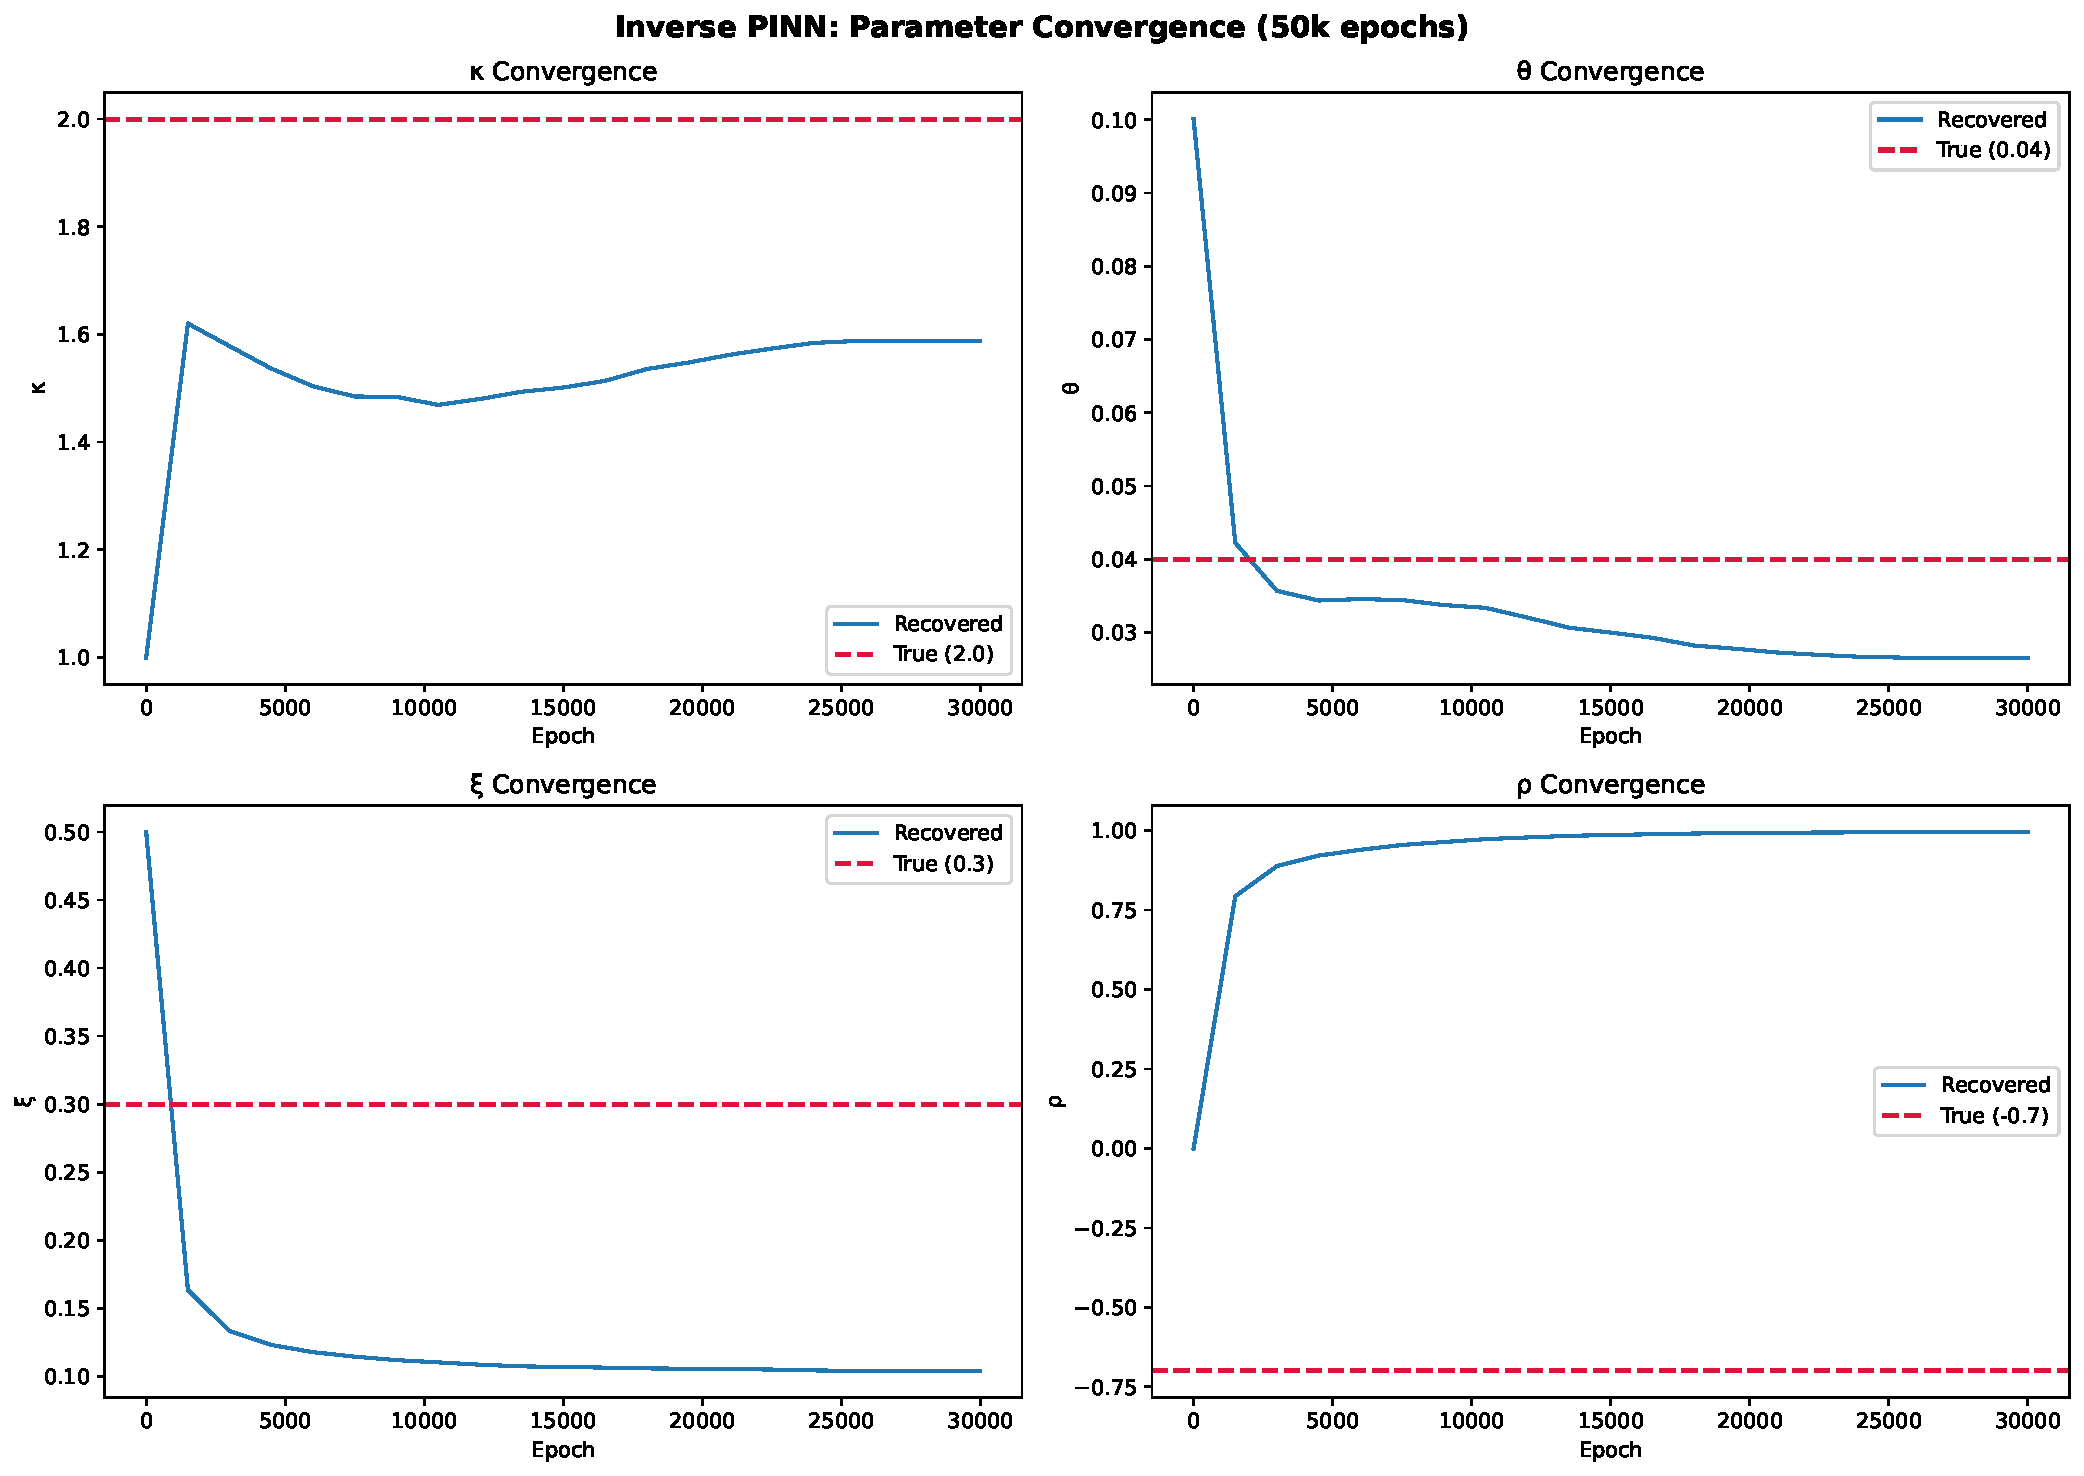
\includegraphics[width=\linewidth]{figures/pinn_inv_params.pdf}
        \caption{Estimated Heston parameters during inverse PINN calibration. The figure shows the evolution of $\kappa$, $\theta$, $\xi$, and $\rho$, giving a direct view of parameter convergence and stability across epochs.}
        \label{fig:pinn_inv_params.pdf}
    \end{subfigure}

    \caption{Inverse PINN calibration diagnostics. The upper panel summarizes loss convergence, while the lower panel shows the corresponding evolution of the calibrated Heston parameters.}
    \label{fig:pinn_inv_diagnostics_panel}
\end{figure}

%%%%%%%%%%%%%%%%%%%%%%%%%%%%%%%%%%%%%%%%%%%%%%%%%%%%%%%%%%%%%%%%%%%%%%%%%%%%
%%%%%%%%%%%%%%%%%%%%%%%%%%%%%%%%%%%%%%%%%%%%%%%%%%%%%%%%%%%%%%%%%%%%%%%%%%%%
%%%%%%%%%%%%%%%%%%%%%%%%%%%%%%%%%%%%%%%%%%%%%%%%%%%%%%%%%%%%%%%%%%%%%%%%%%%%

\begin{figure}[H]
    \centering
    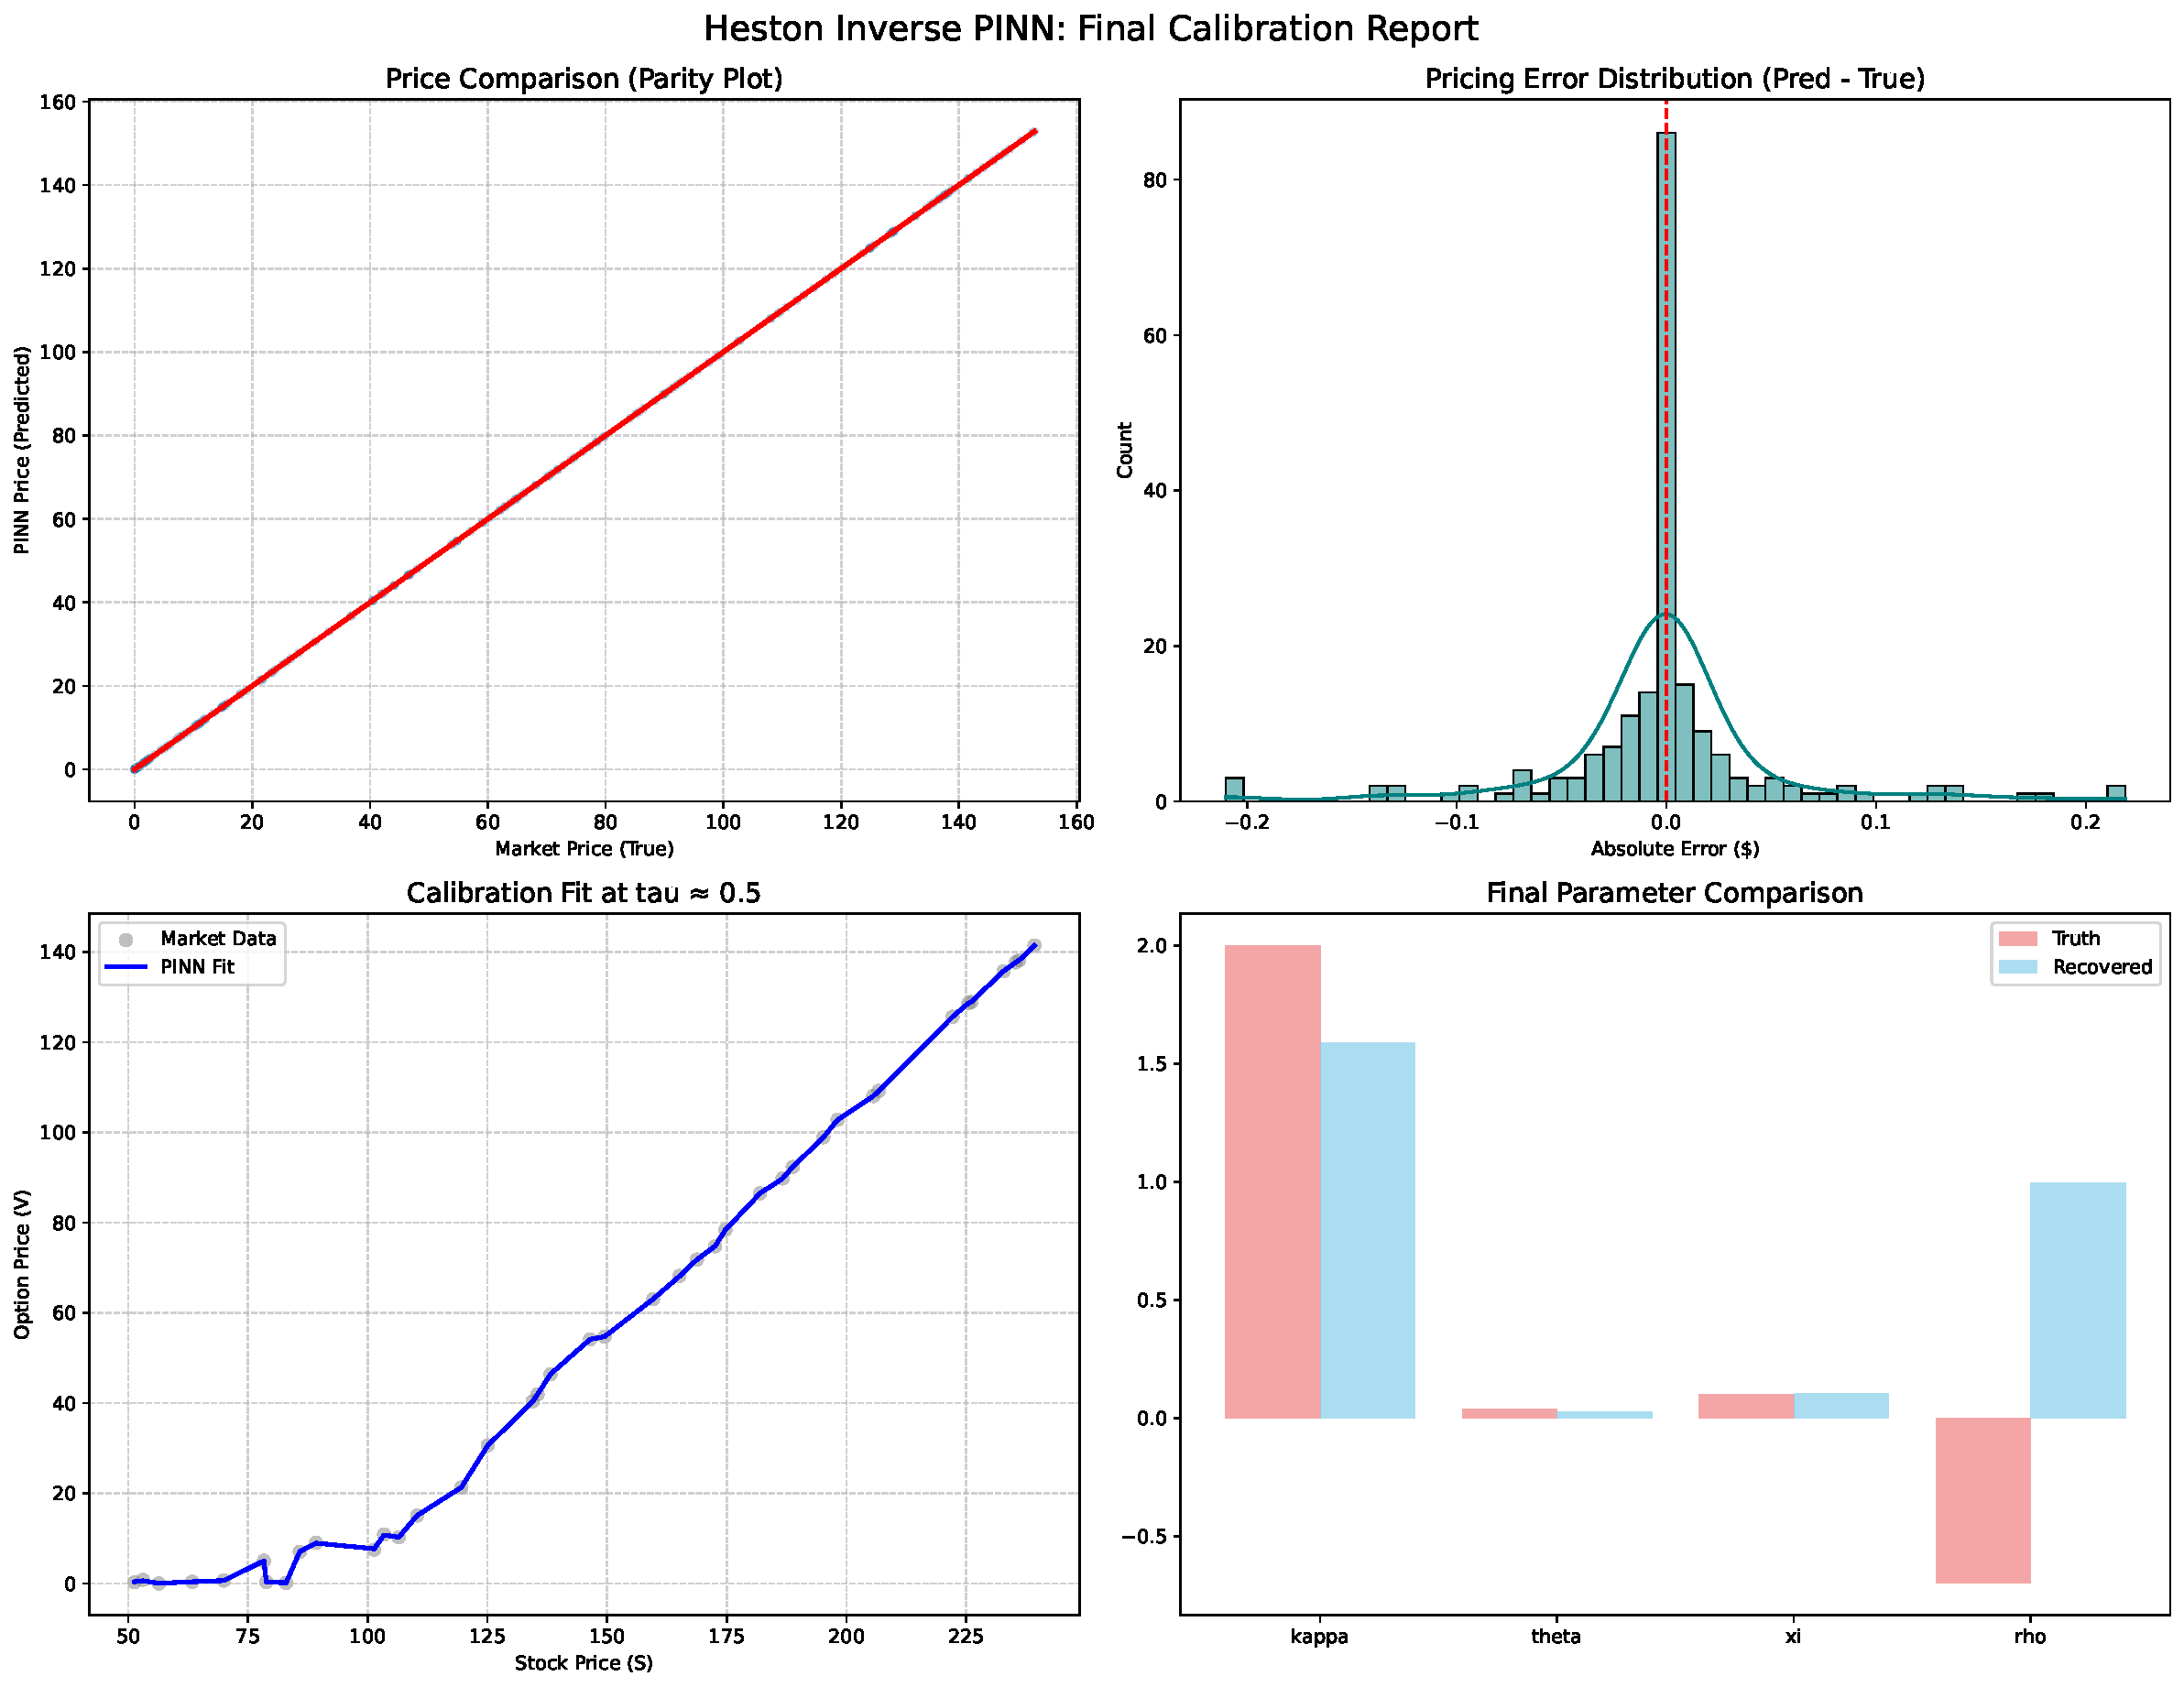
\includegraphics[width=\linewidth]{figures/pinn_inv_final_calibration_report.pdf}
    \caption{Caption}
    \label{fig:placeholder}
\end{figure}

%%%%%%%%%%%%%%%%%%%%%%%%%%%%%%%%%%%%%%%%%%%%%%%%%%%%%%%%%%%%%%%%%%%%%%%%%%%%
%%%%%%%%%%%%%%%%%%%%%%%%%%%%%%%%%%%%%%%%%%%%%%%%%%%%%%%%%%%%%%%%%%%%%%%%%%%%
%%%%%%%%%%%%%%%%%%%%%%%%%%%%%%%%%%%%%%%%%%%%%%%%%%%%%%%%%%%%%%%%%%%%%%%%%%%%

\end{document}